\documentclass{article}
% \usepackage[headsepline]{scrlayer-scrpage}

% \ihead{Levin}
% \ohead{\thepage}
% \pagestyle{scrheadings}
\usepackage{bbm}
\usepackage{amsmath,amsfonts,amsthm,amssymb,amsopn,bm}
\usepackage[margin=.9in]{geometry}
\usepackage{graphicx}
\usepackage{url}
\usepackage[usenames,dvipsnames]{color}
\usepackage{fancyhdr}
\usepackage{multirow}
\usepackage{pythonhighlight}
\usepackage{pgfplots}
\usepackage{pgfplots}
\pgfplotsset{compat=1.11}
\usepackage{minted}
% Default fixed font does not support bold face
\DeclareFixedFont{\ttb}{T1}{txtt}{bx}{n}{12} % for bold
\DeclareFixedFont{\ttm}{T1}{txtt}{m}{n}{12}  % for normal

% Custom colors
\usepackage{color}
\definecolor{deepblue}{rgb}{0,0,0.5}
\definecolor{deepred}{rgb}{0.6,0,0}
\definecolor{deepgreen}{rgb}{0,0.5,0}

\usepackage{listings}

% Python style for highlighting
\newcommand\pythonstyle{\lstset{
language=Python,
basicstyle=\ttm,
otherkeywords={self},             % Add keywords here
keywordstyle=\ttb\color{deepblue},
emph={MyClass,__init__},          % Custom highlighting
emphstyle=\ttb\color{deepred},    % Custom highlighting style
stringstyle=\color{deepgreen},
frame=tb,                         % Any extra options here
showstringspaces=false            % 
}}


% Python environment
\lstnewenvironment{python}[1][]
{
\pythonstyle
\lstset{#1}
}
{}

% Python for external files
\newcommand\pythonexternal[2][]{{
\pythonstyle
\lstinputlisting[#1]{#2}}}

% Python for inline
\newcommand\pythoninline[1]{{\pythonstyle\lstinline!#1!}}

% Some additional tweaking for this package can be made in the preamble. To change the size of each plot and also guarantee backwards compatibility (recommended) add the next line:

\pgfplotsset{width=10cm,compat=1.9}

% This changes the size of each pgfplot figure to 10 centimeters, which is huge; you may use different units (pt, mm, in). The compat parameter is for the code to work on the package version 1.9 or later.

% Since LaTeX was not initially conceived with plotting capabilities in mind, when there are several pgfplot figures in your document or they are very complex, it takes a considerable amount of time to render them. To improve the compiling time you can configure the package to export the figures to separate PDF files and then import them into the document, add the code shown below to the preamble:

\usepgfplotslibrary{external}

\tikzexternalize 

\newcommand{\field}[1]{\mathbb{#1}}
\newcommand{\1}{\mathbf{1}}
\newcommand{\I}{\mathbbm{1}}
\newcommand{\E}{\mathbb{E}} 
\newcommand{\V}{\mathbb{V}} 
\renewcommand{\P}{\mathbb{P}}
 \newcommand{\ind}{\perp\!\!\!\perp}
 \DeclareMathOperator{\rank}{rank}
\newcommand{\R}{\field{R}} % real domain
% \newcommand{\C}{\field{C}} % complex domain
\newcommand{\F}{\field{F}} % functional domain

\newcommand{\T}{^{\textrm T}} % transpose

\def\diag{\text{diag}}

%% operator in linear algebra, functional analysis
\newcommand{\inner}[2]{#1\cdot #2}
\newcommand{\norm}[1]{\left\|#1\right\|}
\newcommand{\twonorm}[1]{\|#1\|_2^2}
% operator in functios, maps such as M: domain1 --> domain 2
\newcommand{\Map}[1]{\mathcal{#1}}
\renewcommand{\theenumi}{\alph{enumi}} 

\newcommand{\Perp}{\perp \! \! \! \perp}

\newcommand\independent{\protect\mathpalette{\protect\independenT}{\perp}}
\def\independenT#1#2{\mathrel{\rlap{$#1#2$}\mkern2mu{#1#2}}}
\newcommand{\vct}[1]{\boldsymbol{#1}} % vector
\newcommand{\mat}[1]{\boldsymbol{#1}} % matrix
\newcommand{\cst}[1]{\mathsf{#1}} % constant
\newcommand{\ProbOpr}[1]{\mathbb{#1}}
\newcommand{\points}[1]{\small\textcolor{magenta}{\emph{[#1 points]}} \normalsize}
\date{{}}

\setlength\parindent{0px}

\begin{document}
\title{Homework \#3}
\author{\normalsize{Spring 2020, CSE 546: Machine Learning}\\
\normalsize{\bf Roman Levin} \\
\normalsize{\bf 1721898} \\
}
\maketitle
Collaborators: compared answers with Tyler Chen, Diya Sashidhar, Katherine Owens

\subsection*{Conceptual Questions}
\noindent\rule{\textwidth}{1pt}

A.1 {\bf Solution:}\\
\begin{enumerate}
    \item {\bf True} (yes, since only $k$ eigenvalues of the covariance matrix are nonzero)
    \item {\bf False} (SVM just maximizes the margin, it does not mean the generalization error is optimal among linear models)
    \item {\bf True} (since the bootstrap sampling is with replacement)
    \item {\bf False} (the columns of $V$ are the eigenvectors, not the rows)
    \item {\bf False} (not necessarily, new PCA coordinates could sometimes be very uninterpretable)
    \item {\bf False} ($k=n$ where $n$ is the number of samples results in zero objective and in only one point belonging to each cluster giving no new insights into the data)
    \item {\bf Decrease $\sigma$} (Decreasing $\sigma$ makes the model more expressive.)
\end{enumerate}

\noindent\rule{\textwidth}{1pt}
\subsection*{Kernels and the Bootstrap}
\noindent\rule{\textwidth}{1pt}
A.2 {\bf Solution:}\\
By definition of $\phi(x)$, we have:
$$
\boxed{\phi(x)\phi(x') = \sum_{i=0}^\infty \frac{1}{\sqrt{i!}}e^{-\frac{x^2}{2}}x^i \frac{1}{\sqrt{i!}}e^{-\frac{x'^2}{2}}x'^i =  e^{-\frac{x^2+x'^2}{2}}\sum_{i=0}^\infty \frac{1}{i!}(xx')^i = e^{-\frac{x^2+x'^2}{2}}e^{xx'} = e^{-\frac{(x-x')^2}{2}} \qquad \Box}
$$
\noindent\rule{\textwidth}{1pt}

\noindent\rule{\textwidth}{1pt}
\\
A.3 {\bf Solution:}\\
\begin{enumerate}
    \item Best polynomial kernel parameters: $\lambda = 0.001, d = 17.0$\\
    Best rbf kernel parameters: $\lambda = 0.0001, \gamma = 5.340266090876008$
    \item See Figure 1.
        \begin{figure}[h!]
            \centering
            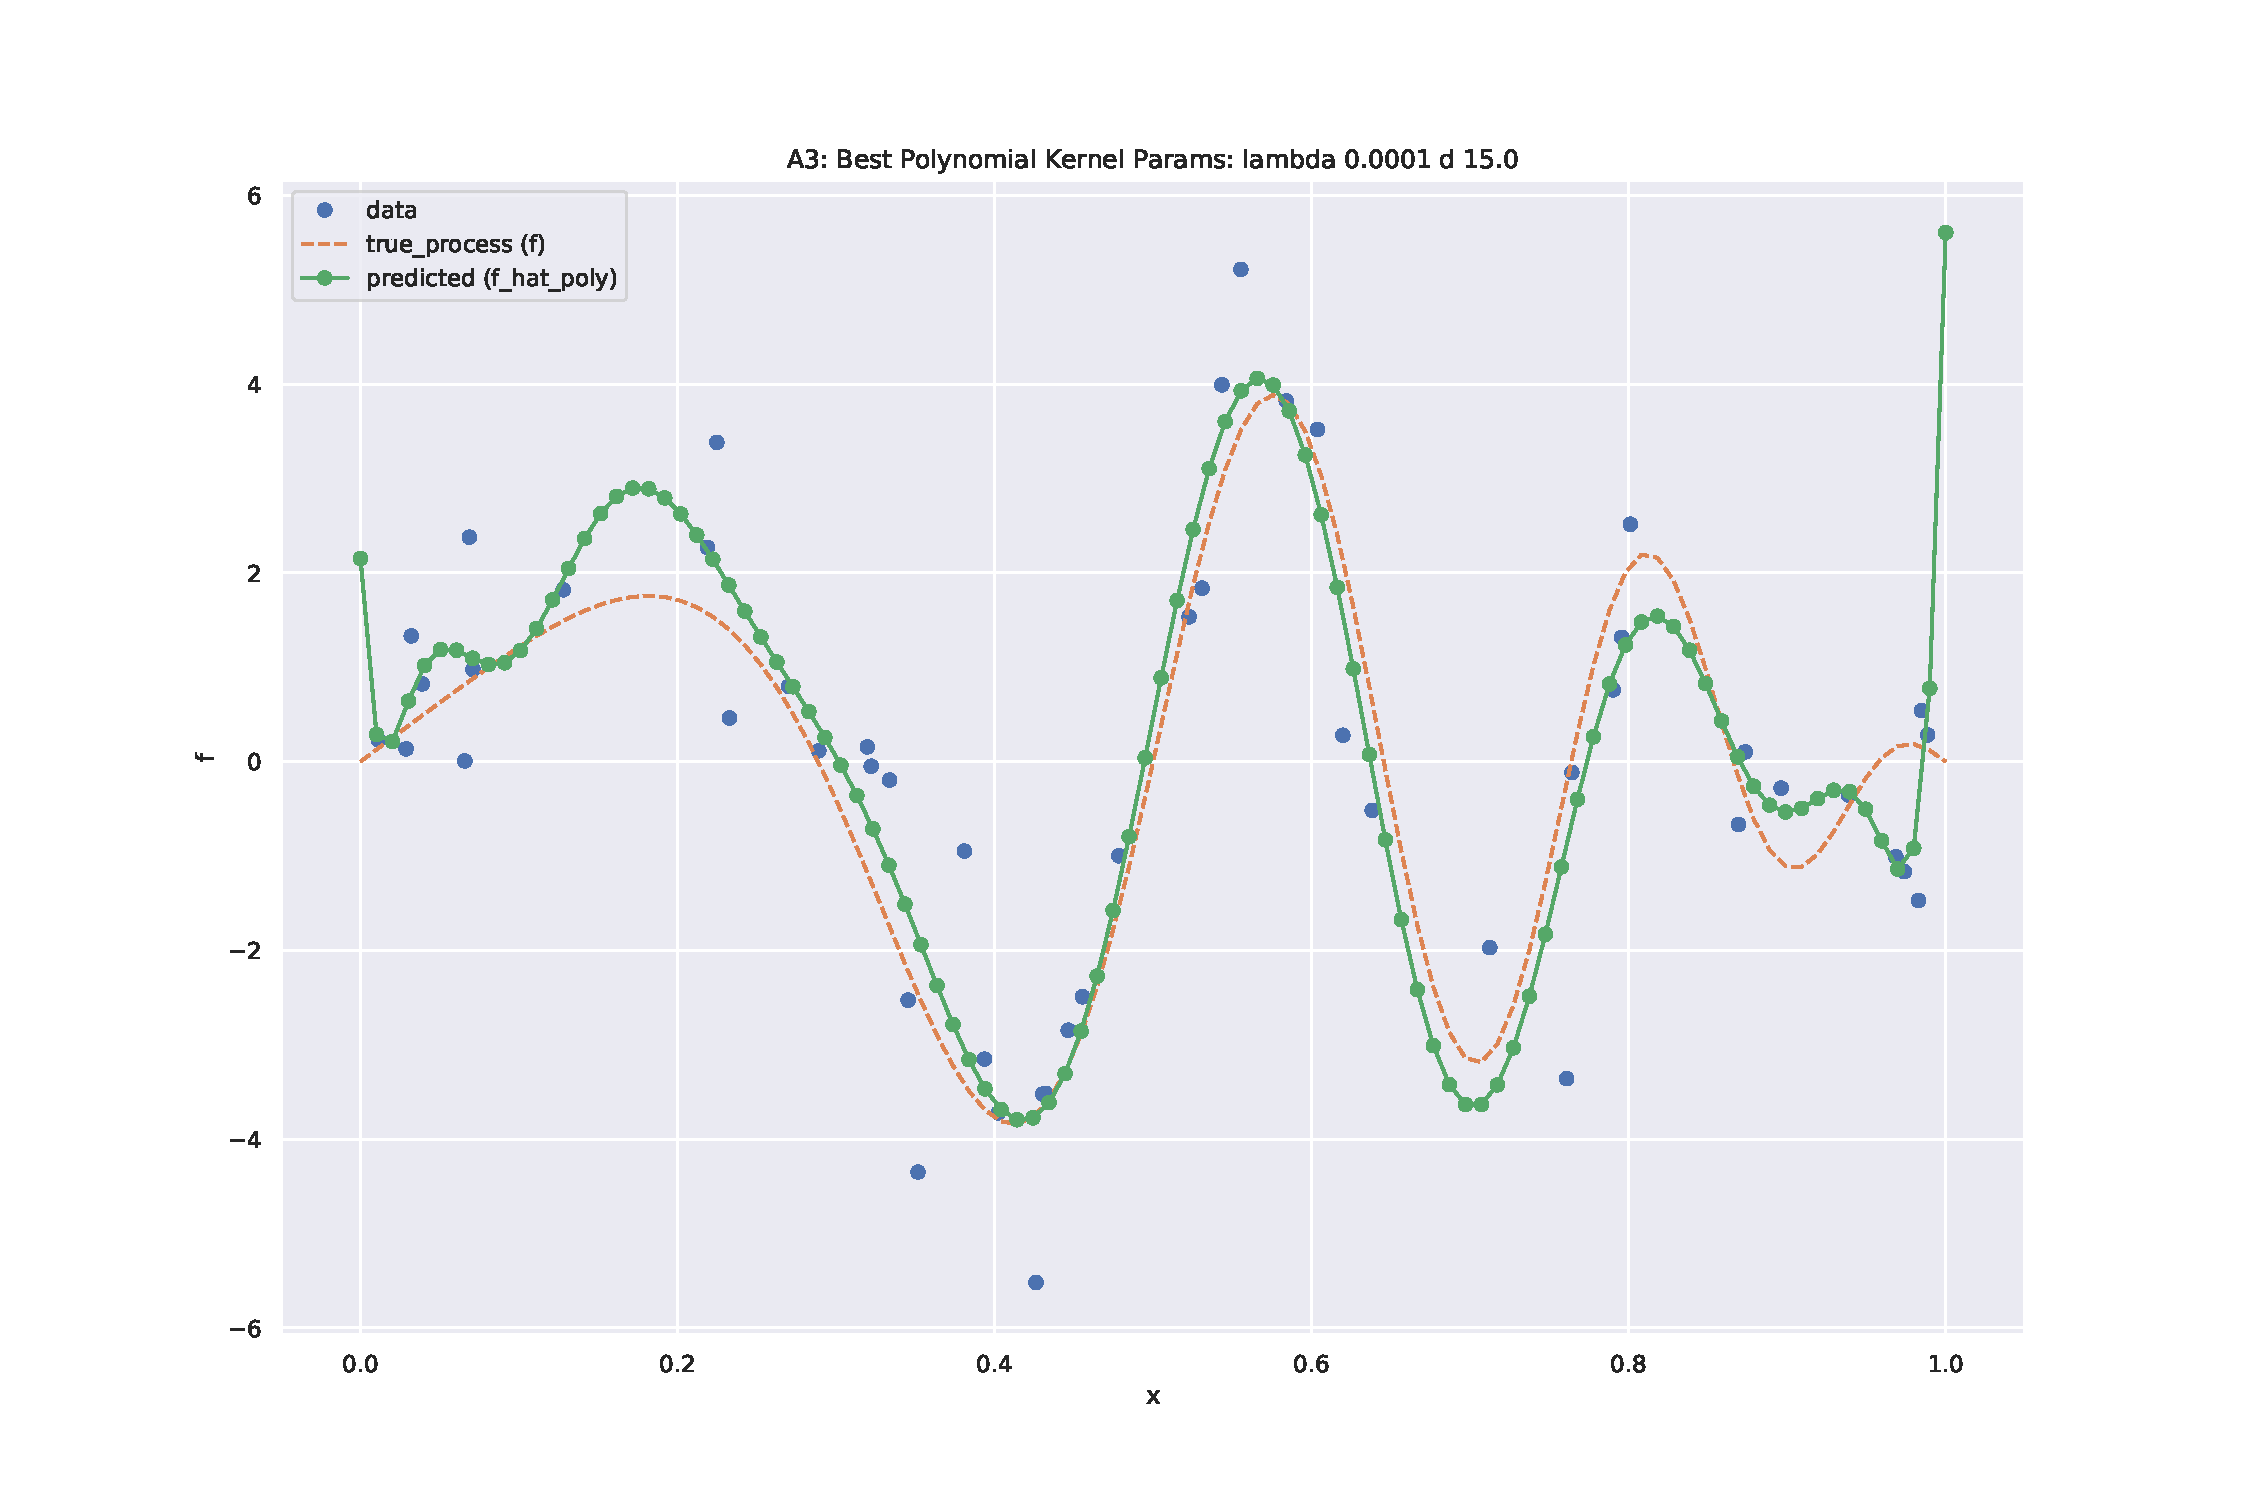
\includegraphics[width=0.49\textwidth]{hw3/code/figures/A3b_poly.pdf}
            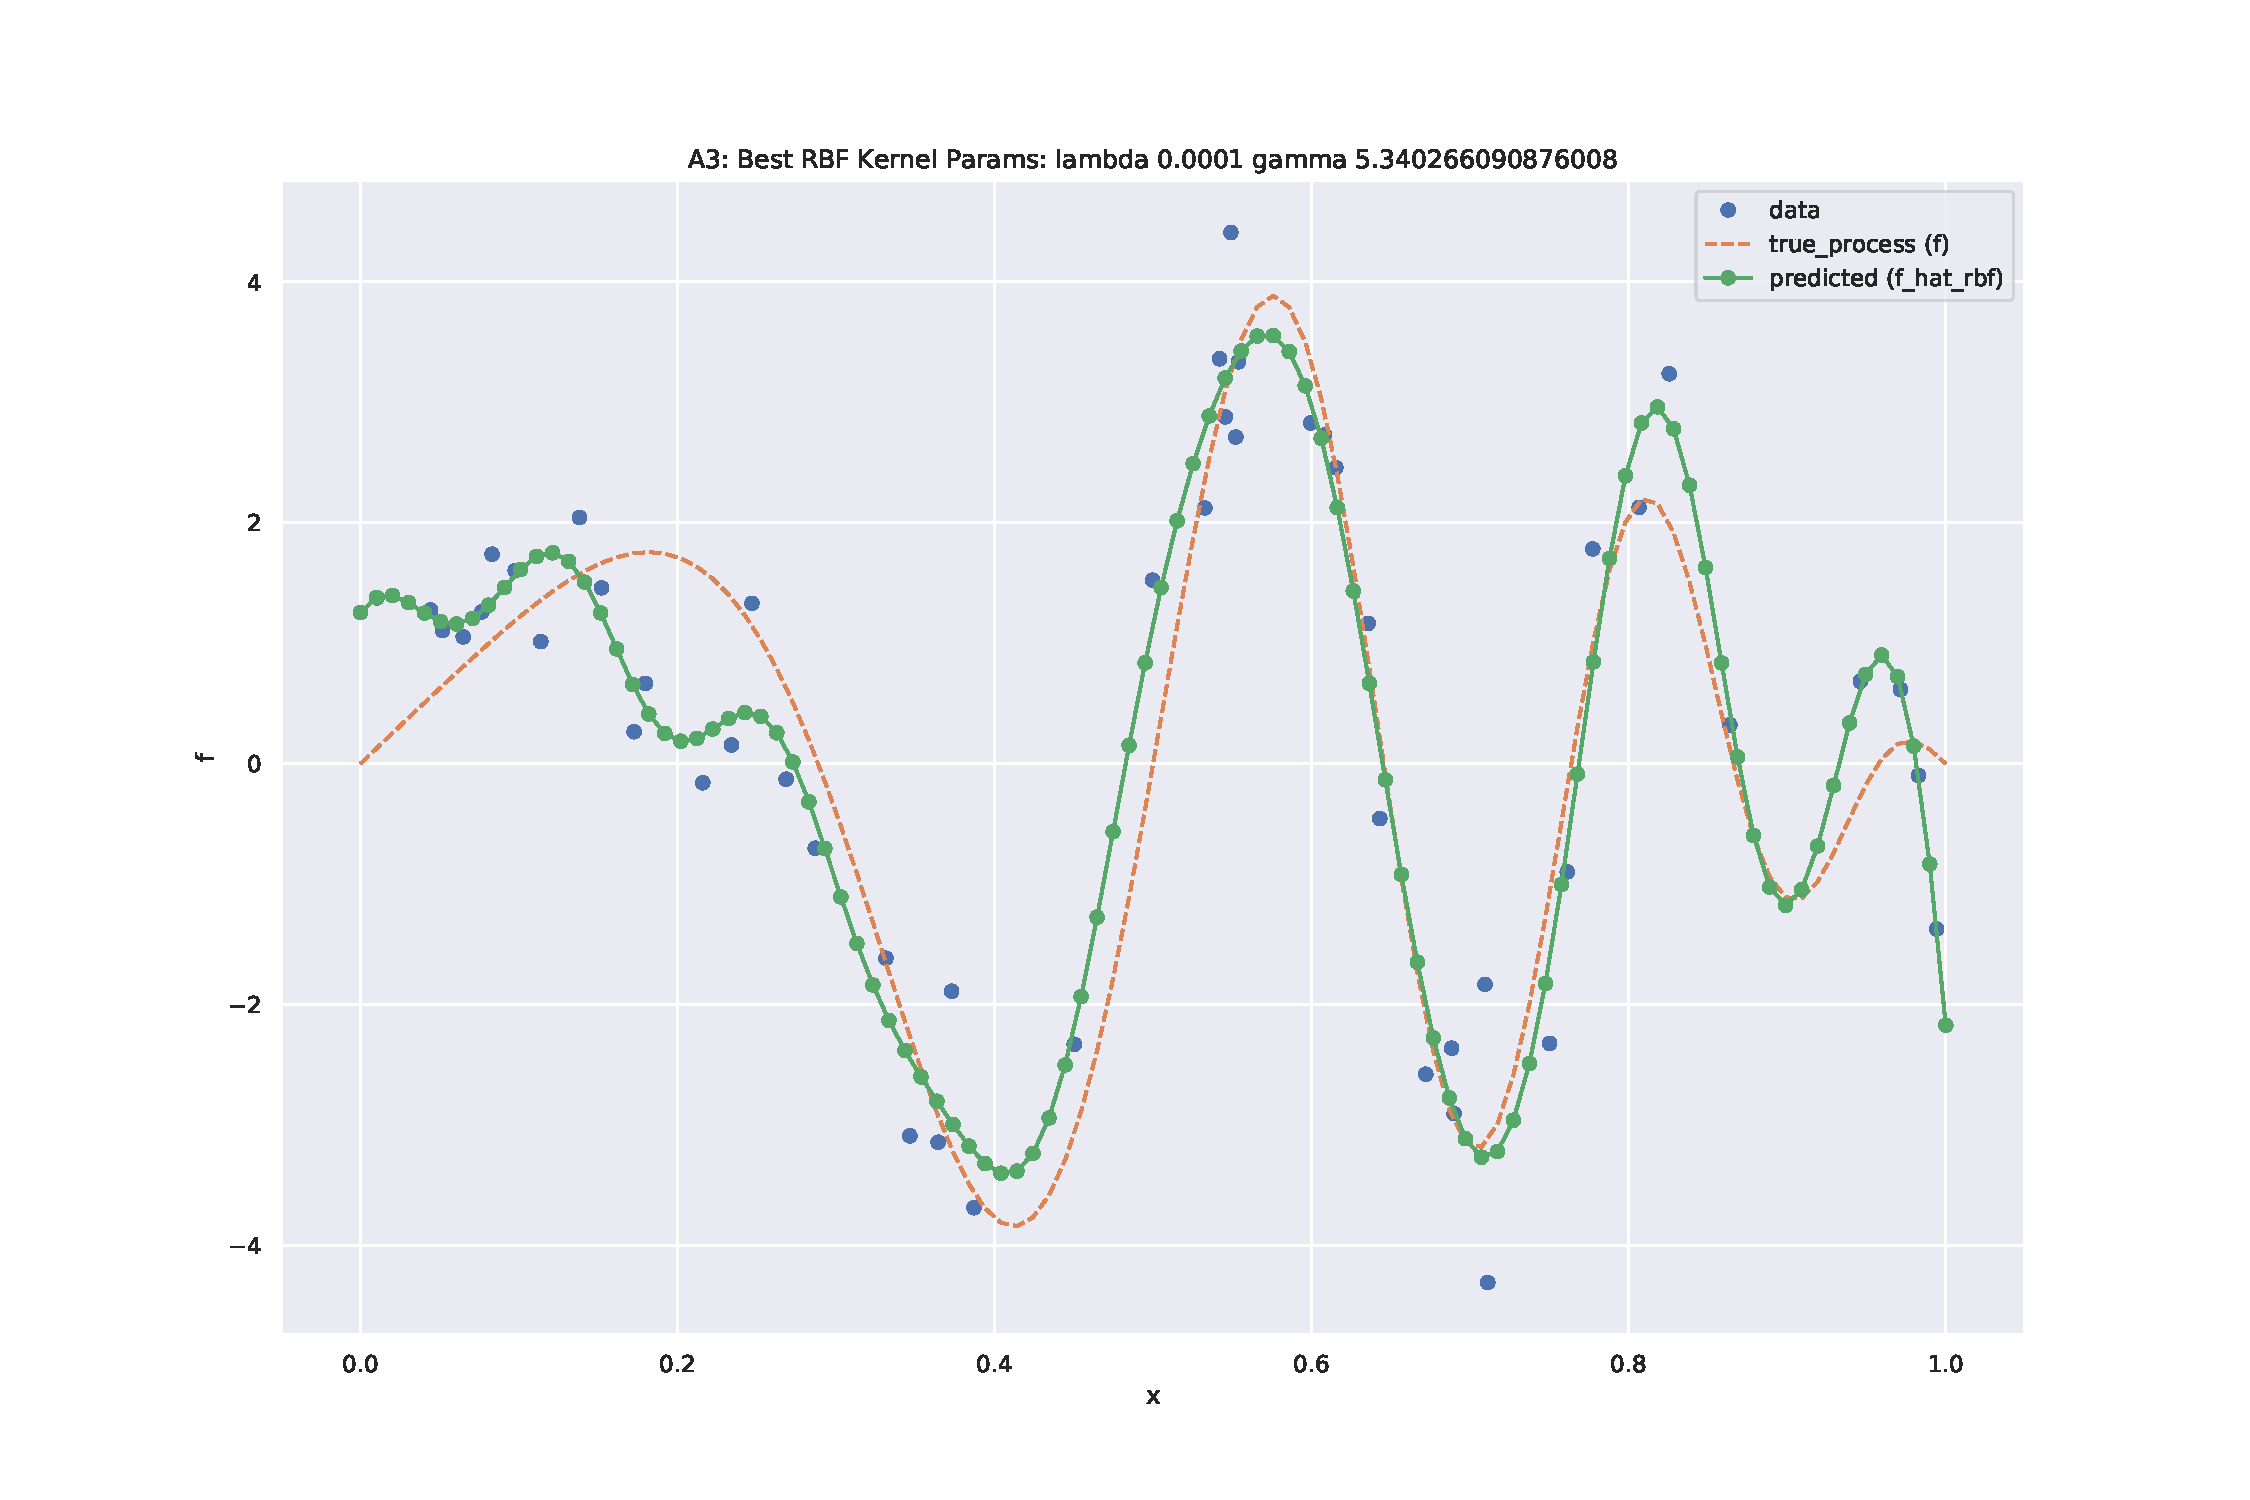
\includegraphics[width=0.49\textwidth]{hw3/code/figures/A3b_rbf.pdf}
            \caption{Problem A3.b Left: Polynomial kernel model, Right: Rbf kernel model}
            \label{figure:a4}
        \end{figure}
    \item See Figure 2.
        \begin{figure}[h!]
            \centering
            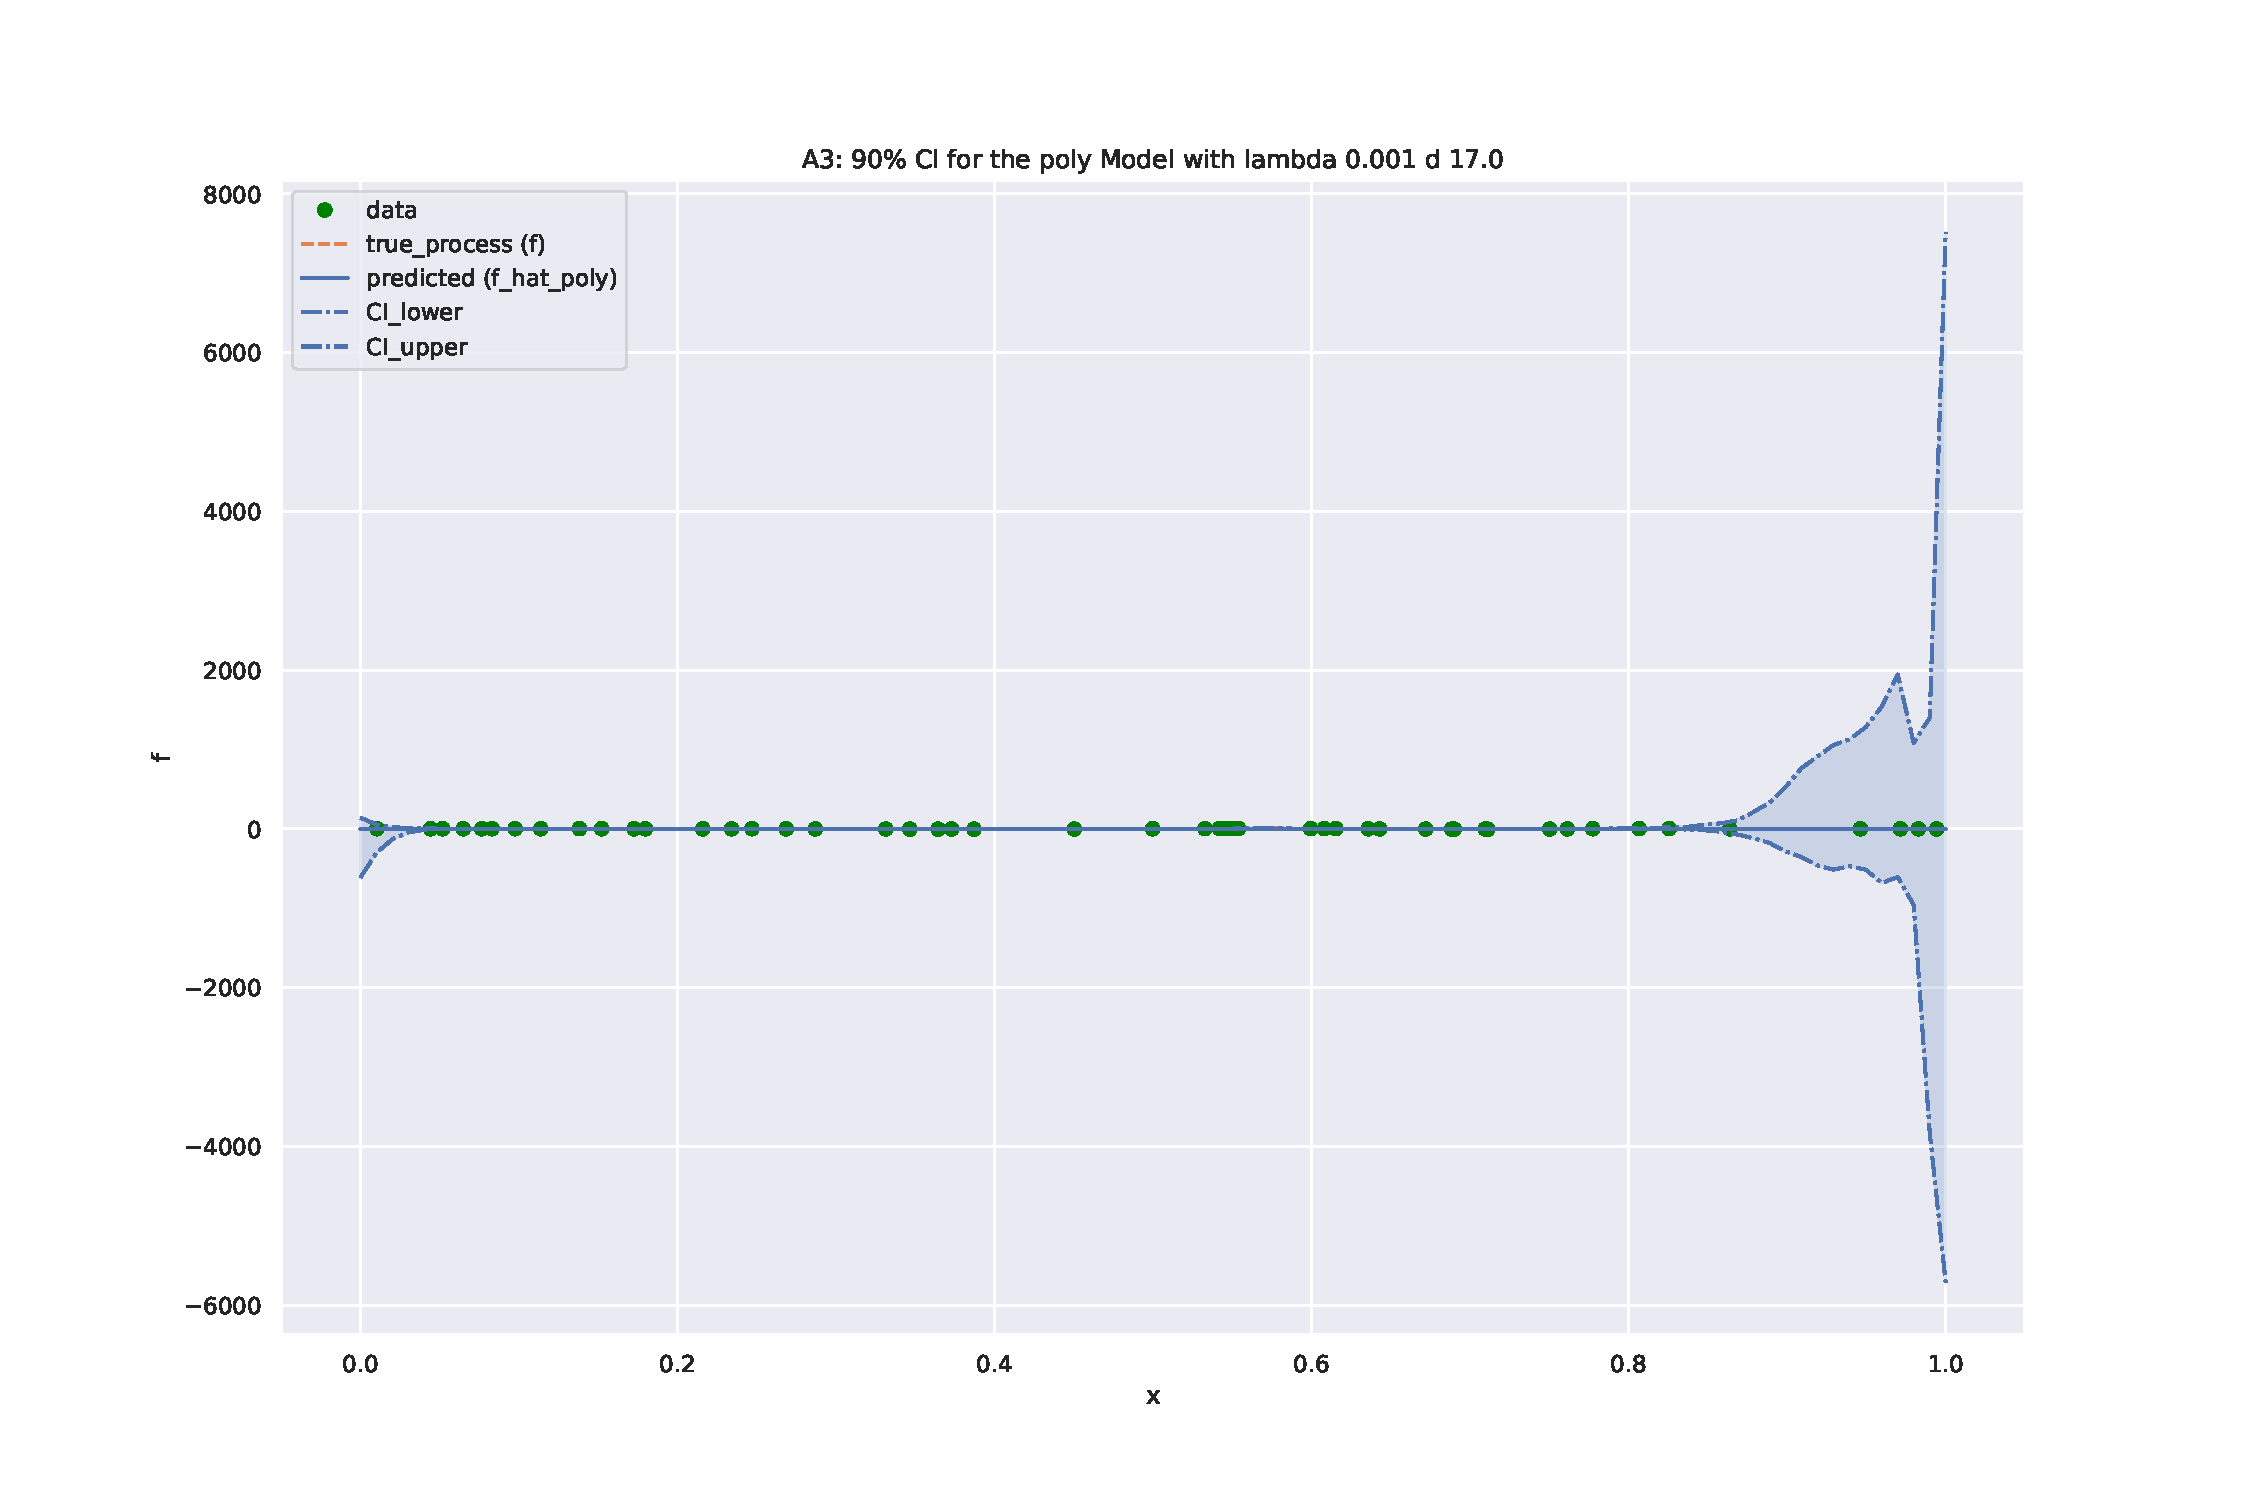
\includegraphics[width=0.49\textwidth]{hw3/code/figures/A3c_poly.pdf}
            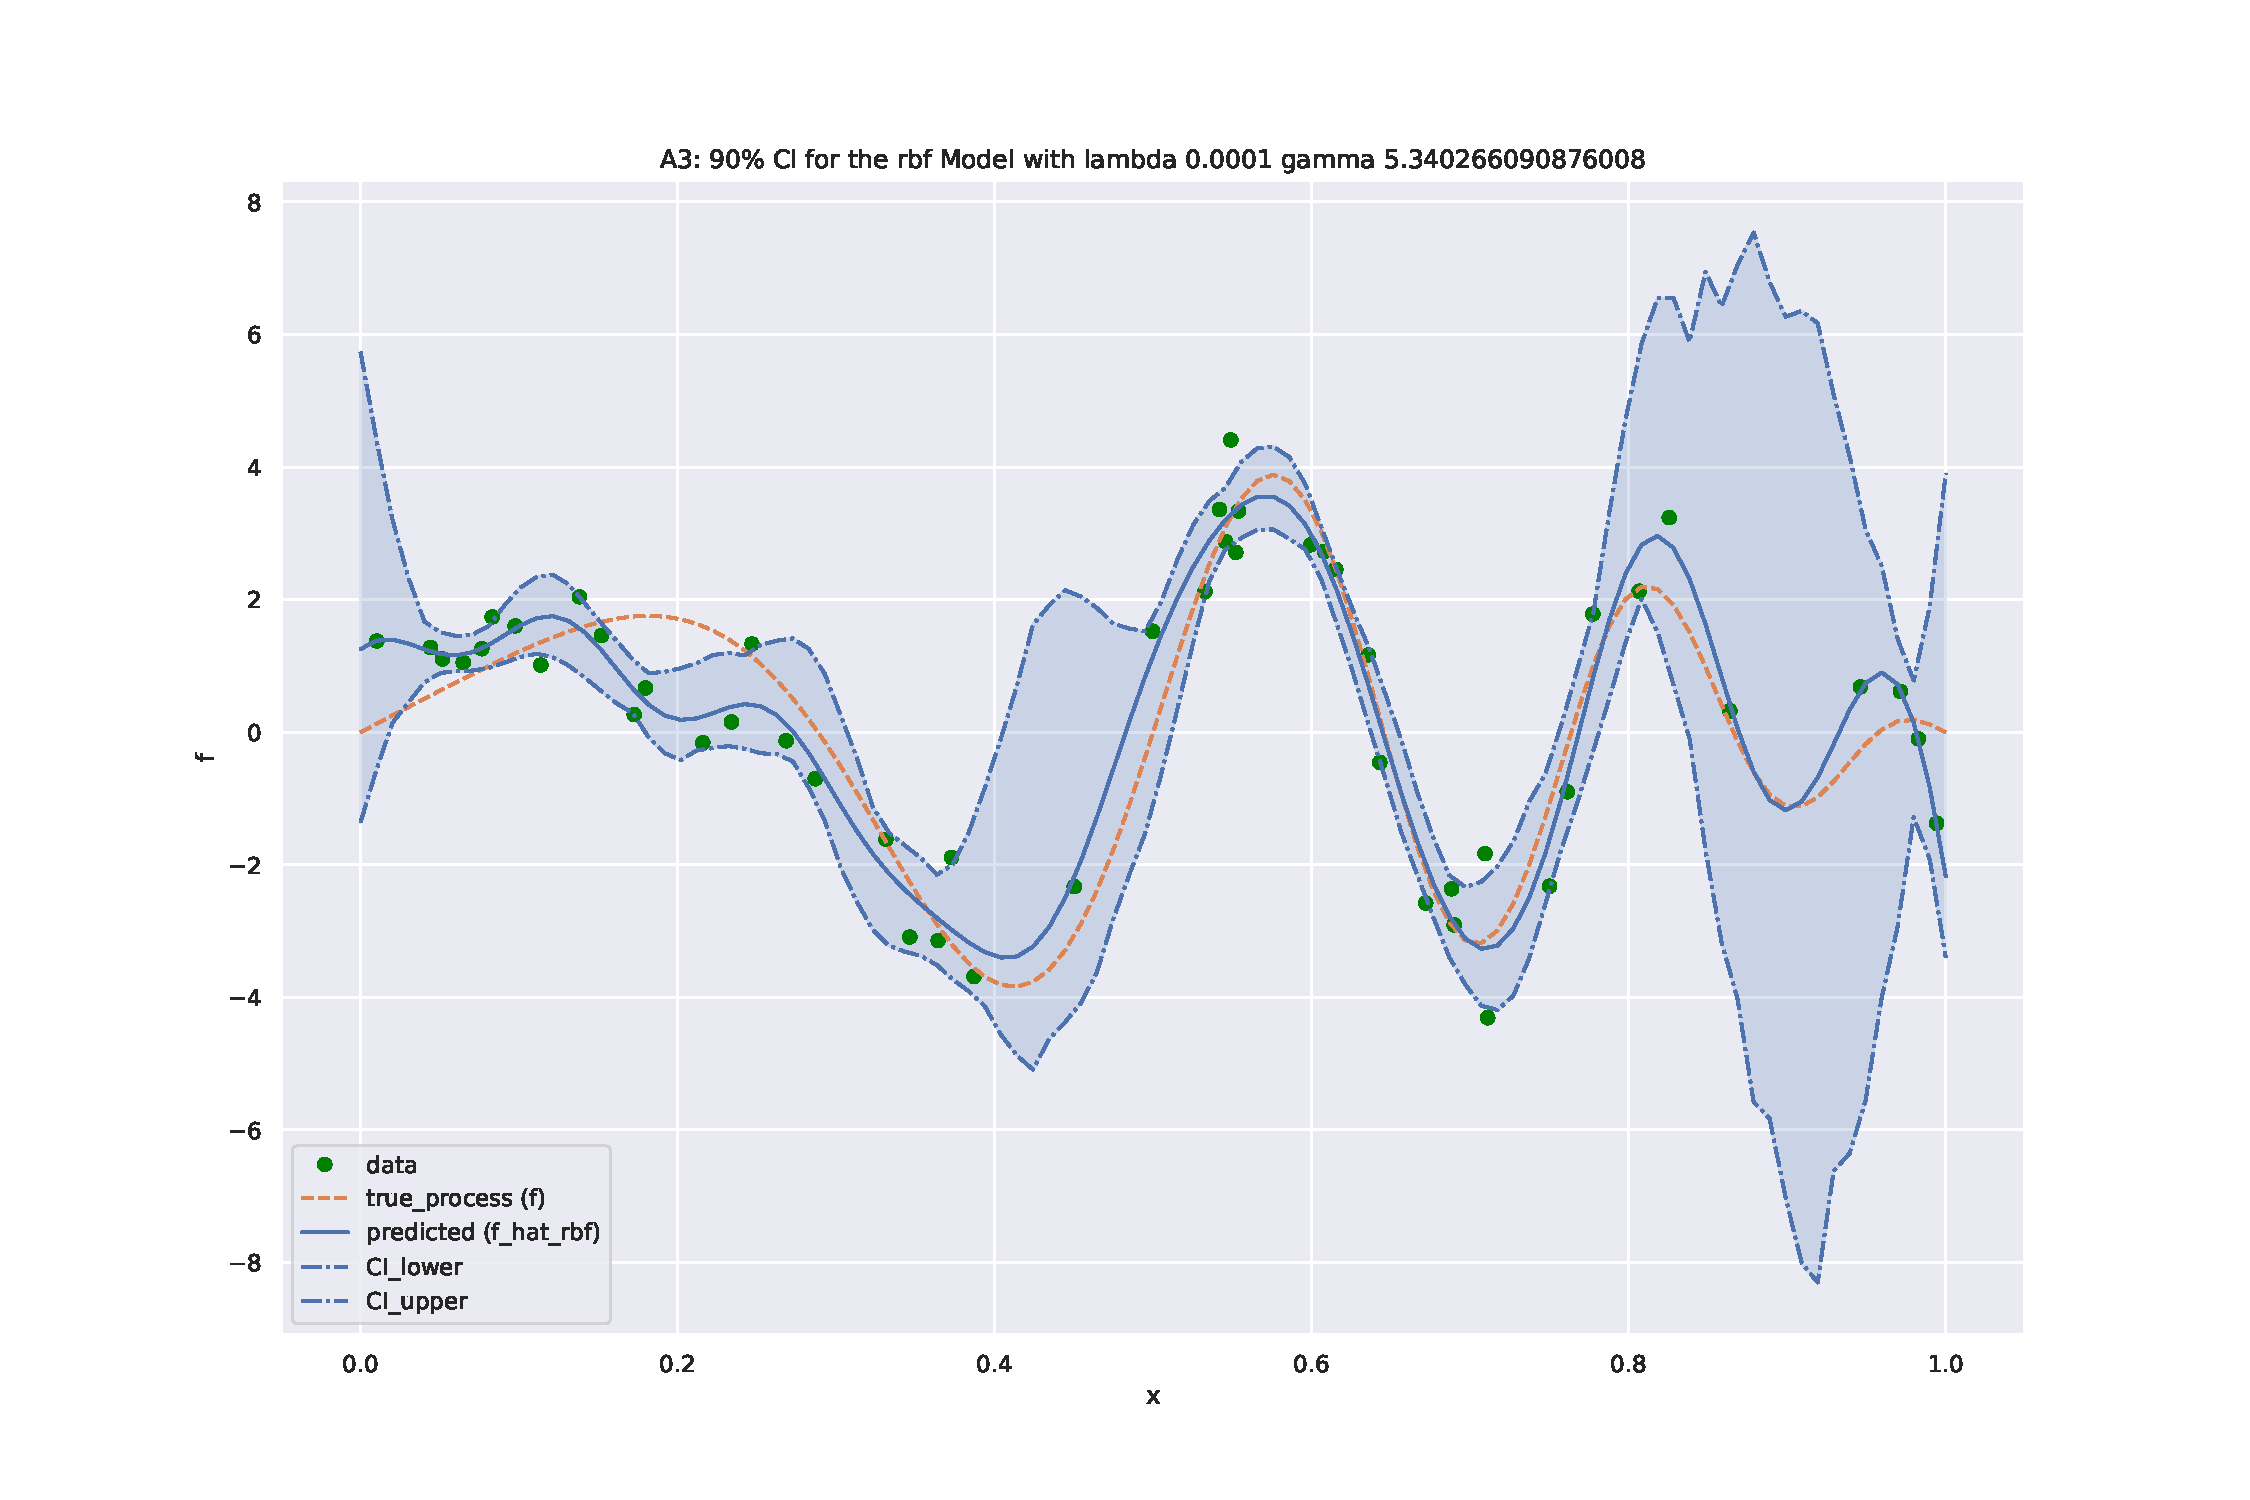
\includegraphics[width=0.49\textwidth]{hw3/code/figures/A3c_rbf.pdf}
            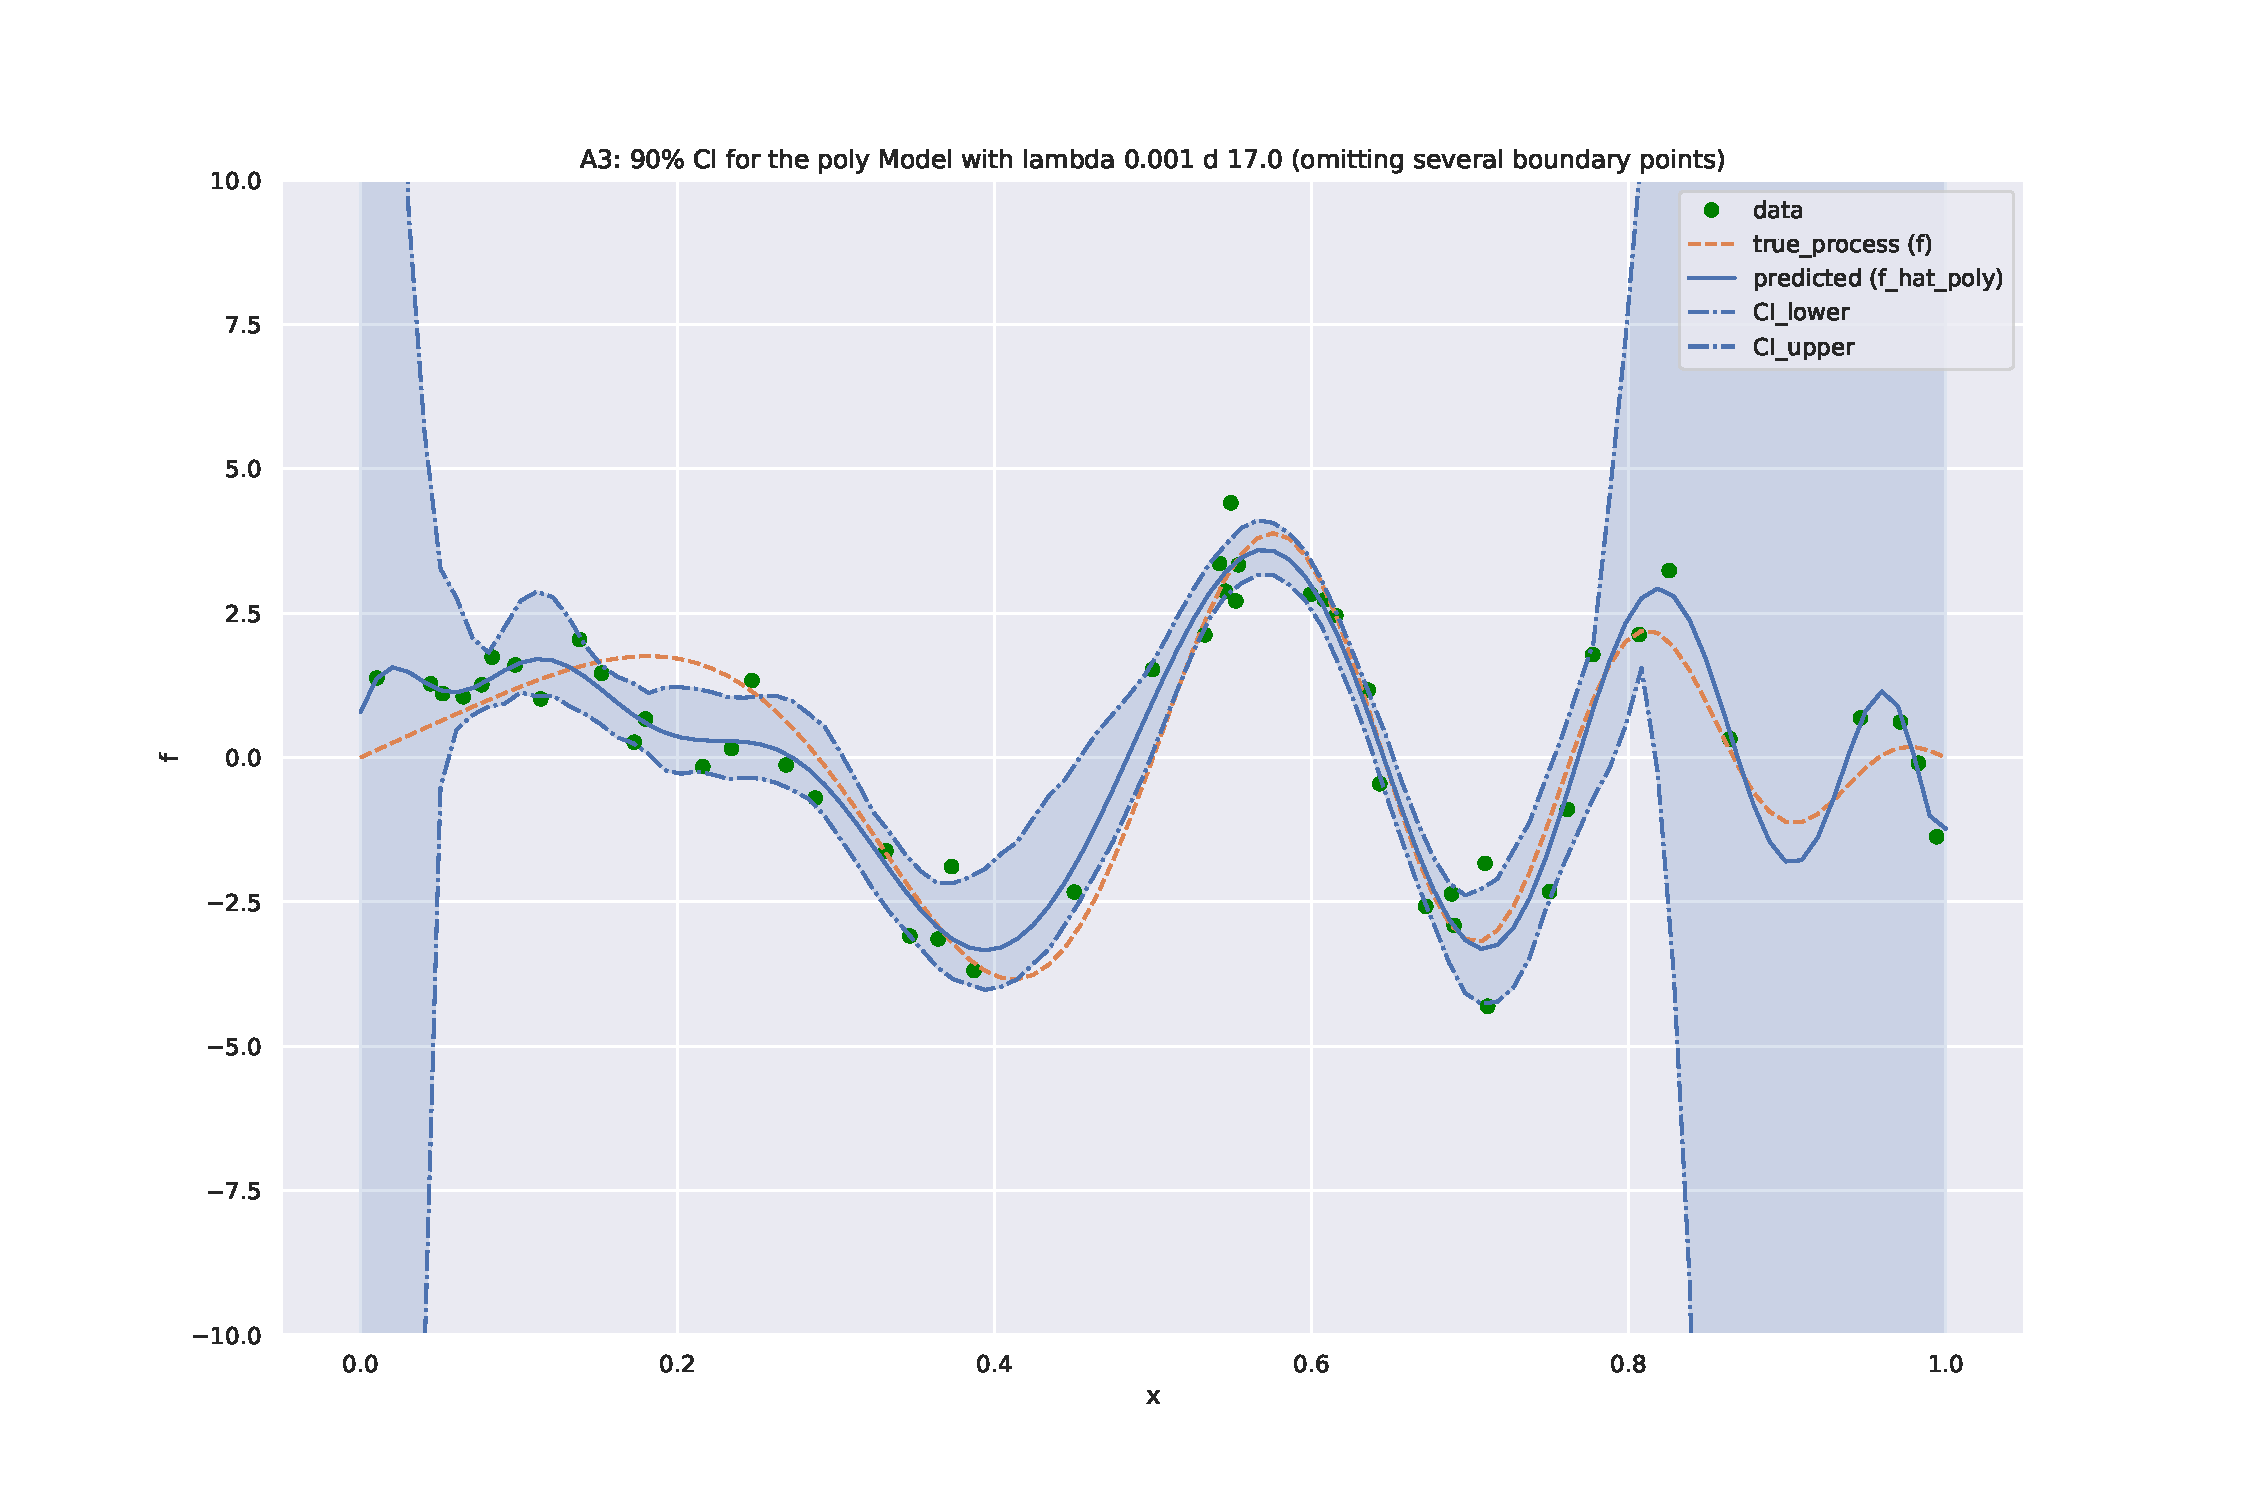
\includegraphics[width=0.6\textwidth]{hw3/code/figures/A3c_poly_zoomed.pdf}
            \caption{Problem A3.c Bootstrap Confidence Intervals. Top Left: Polynomial kernel model, Top Right: Rbf kernel model, Bottom: Zoomed-in version of the polynomial kernel graph, since on the boundaries it is very unstable.}
            \label{figure:a4}
        \end{figure}
    \item Best polynomial kernel parameters for $n=300$: $\lambda = 0.001 d = 16.0$\\
    Best rbf kernel parameters for $n=300$: $\lambda = 0.01, \gamma =  5.131332212328231$\\
    See Figures 3 and 4.
        \begin{figure}[h!]
            \centering
            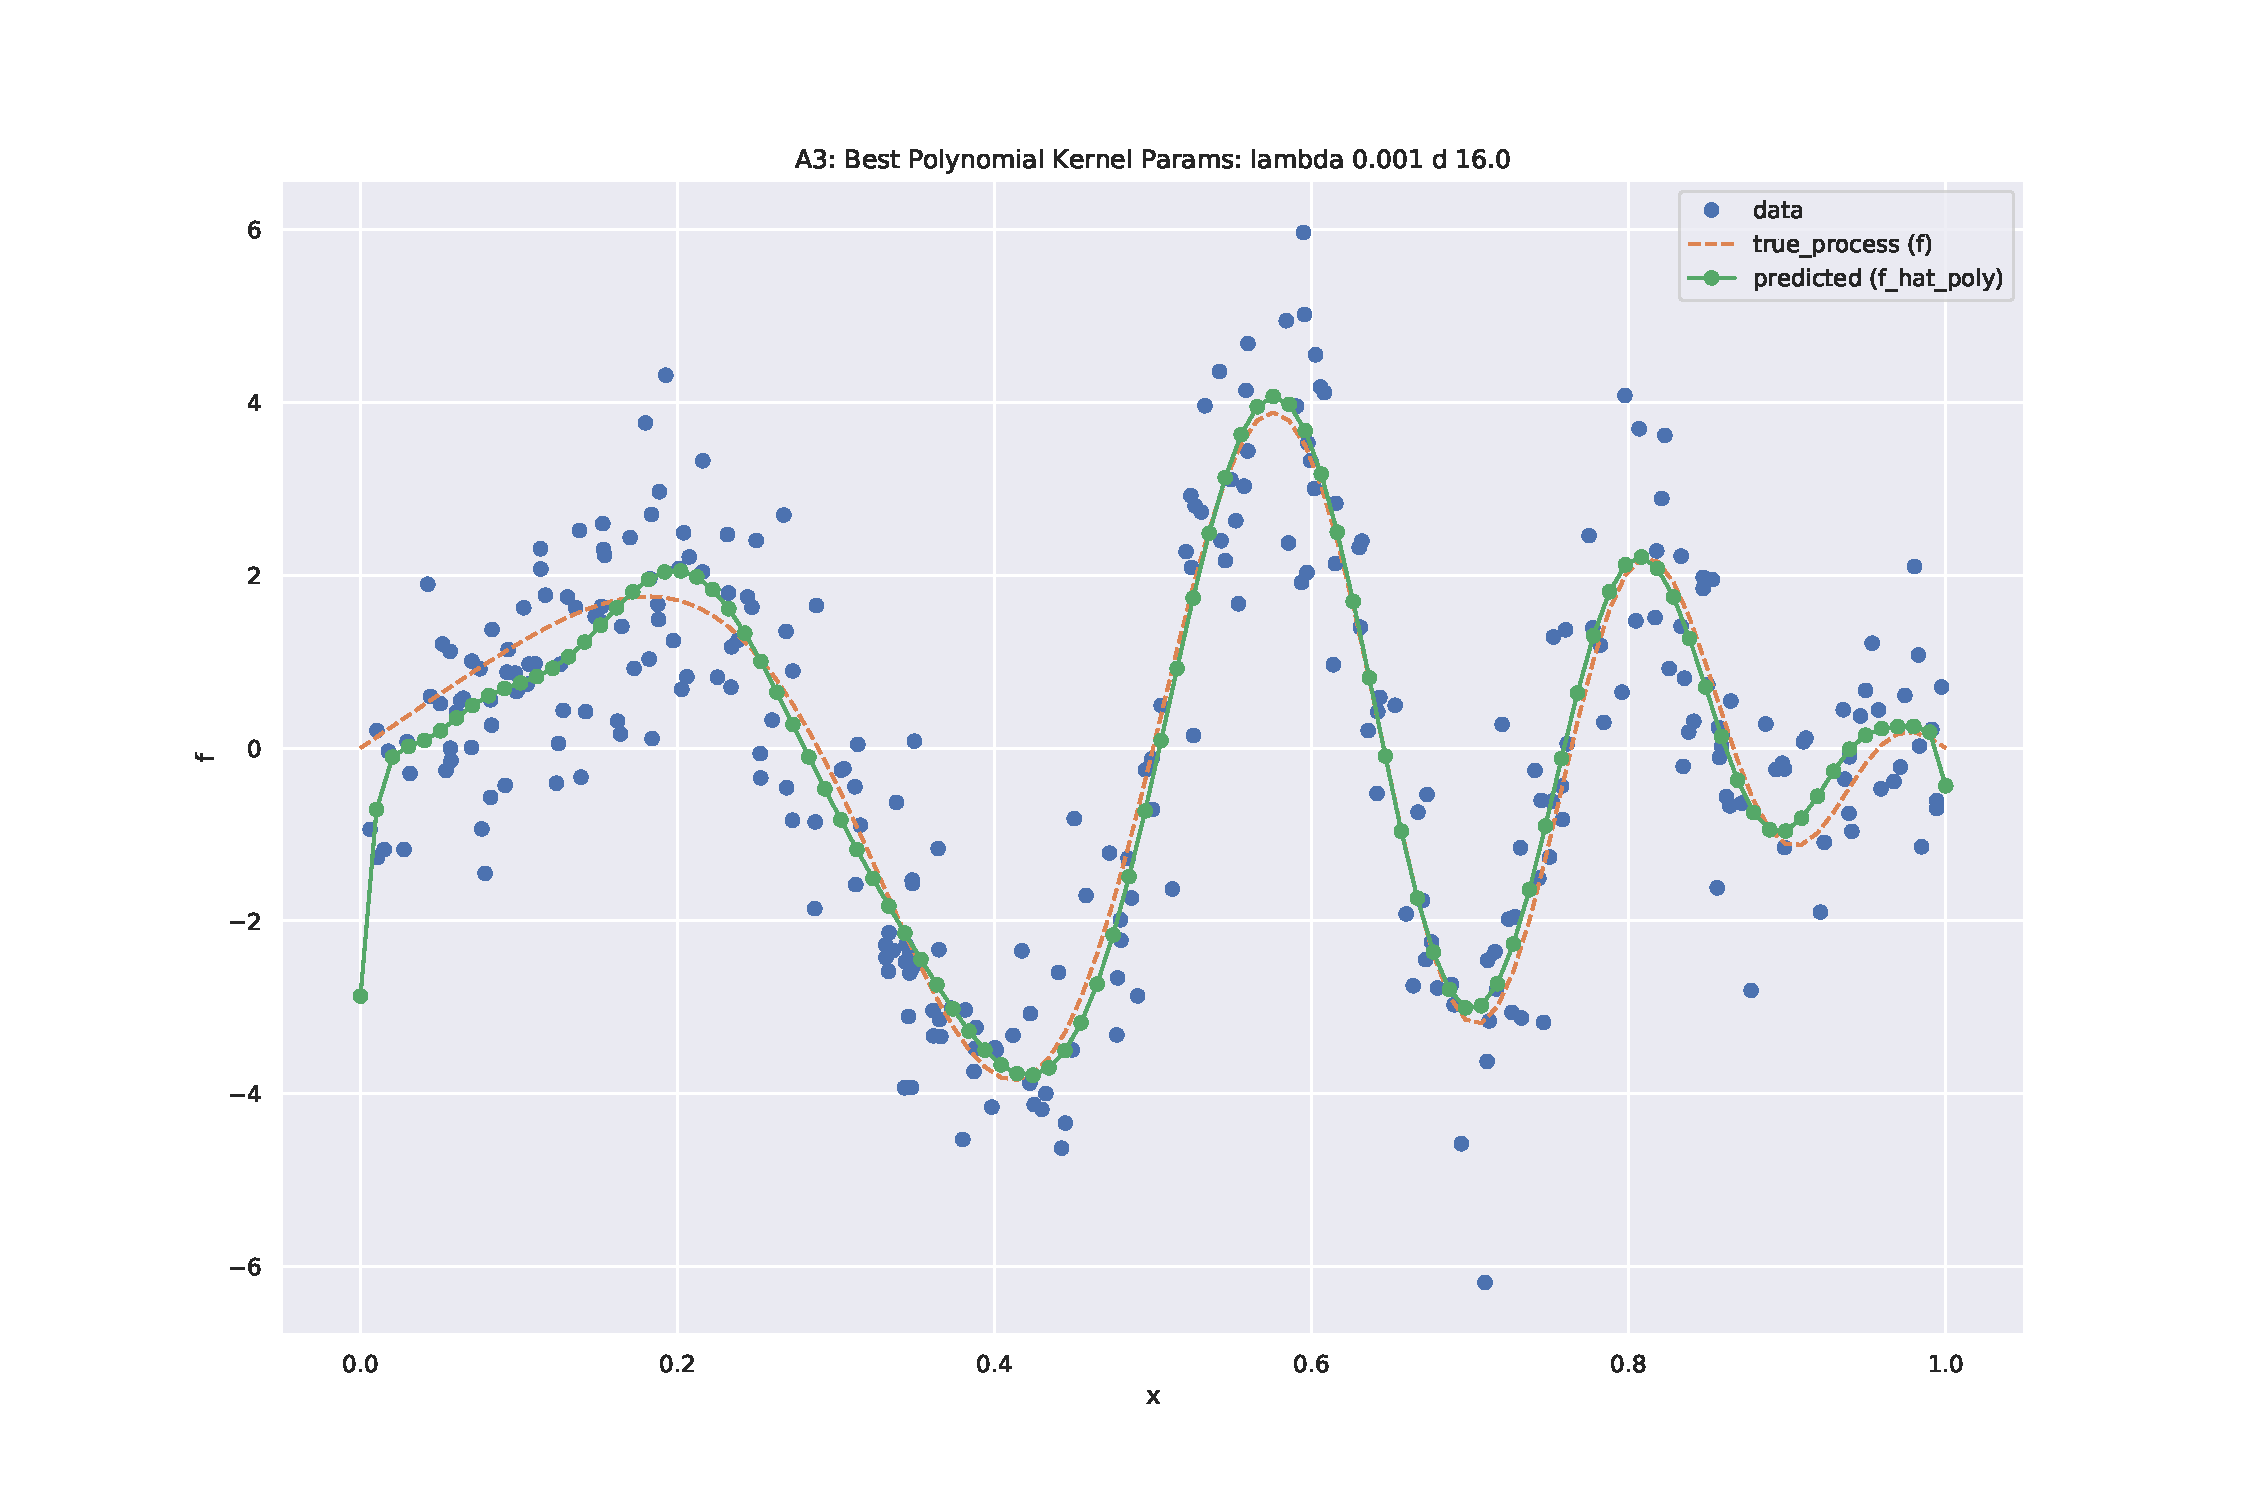
\includegraphics[width=0.49\textwidth]{hw3/code/figures/A3db_poly.pdf}
            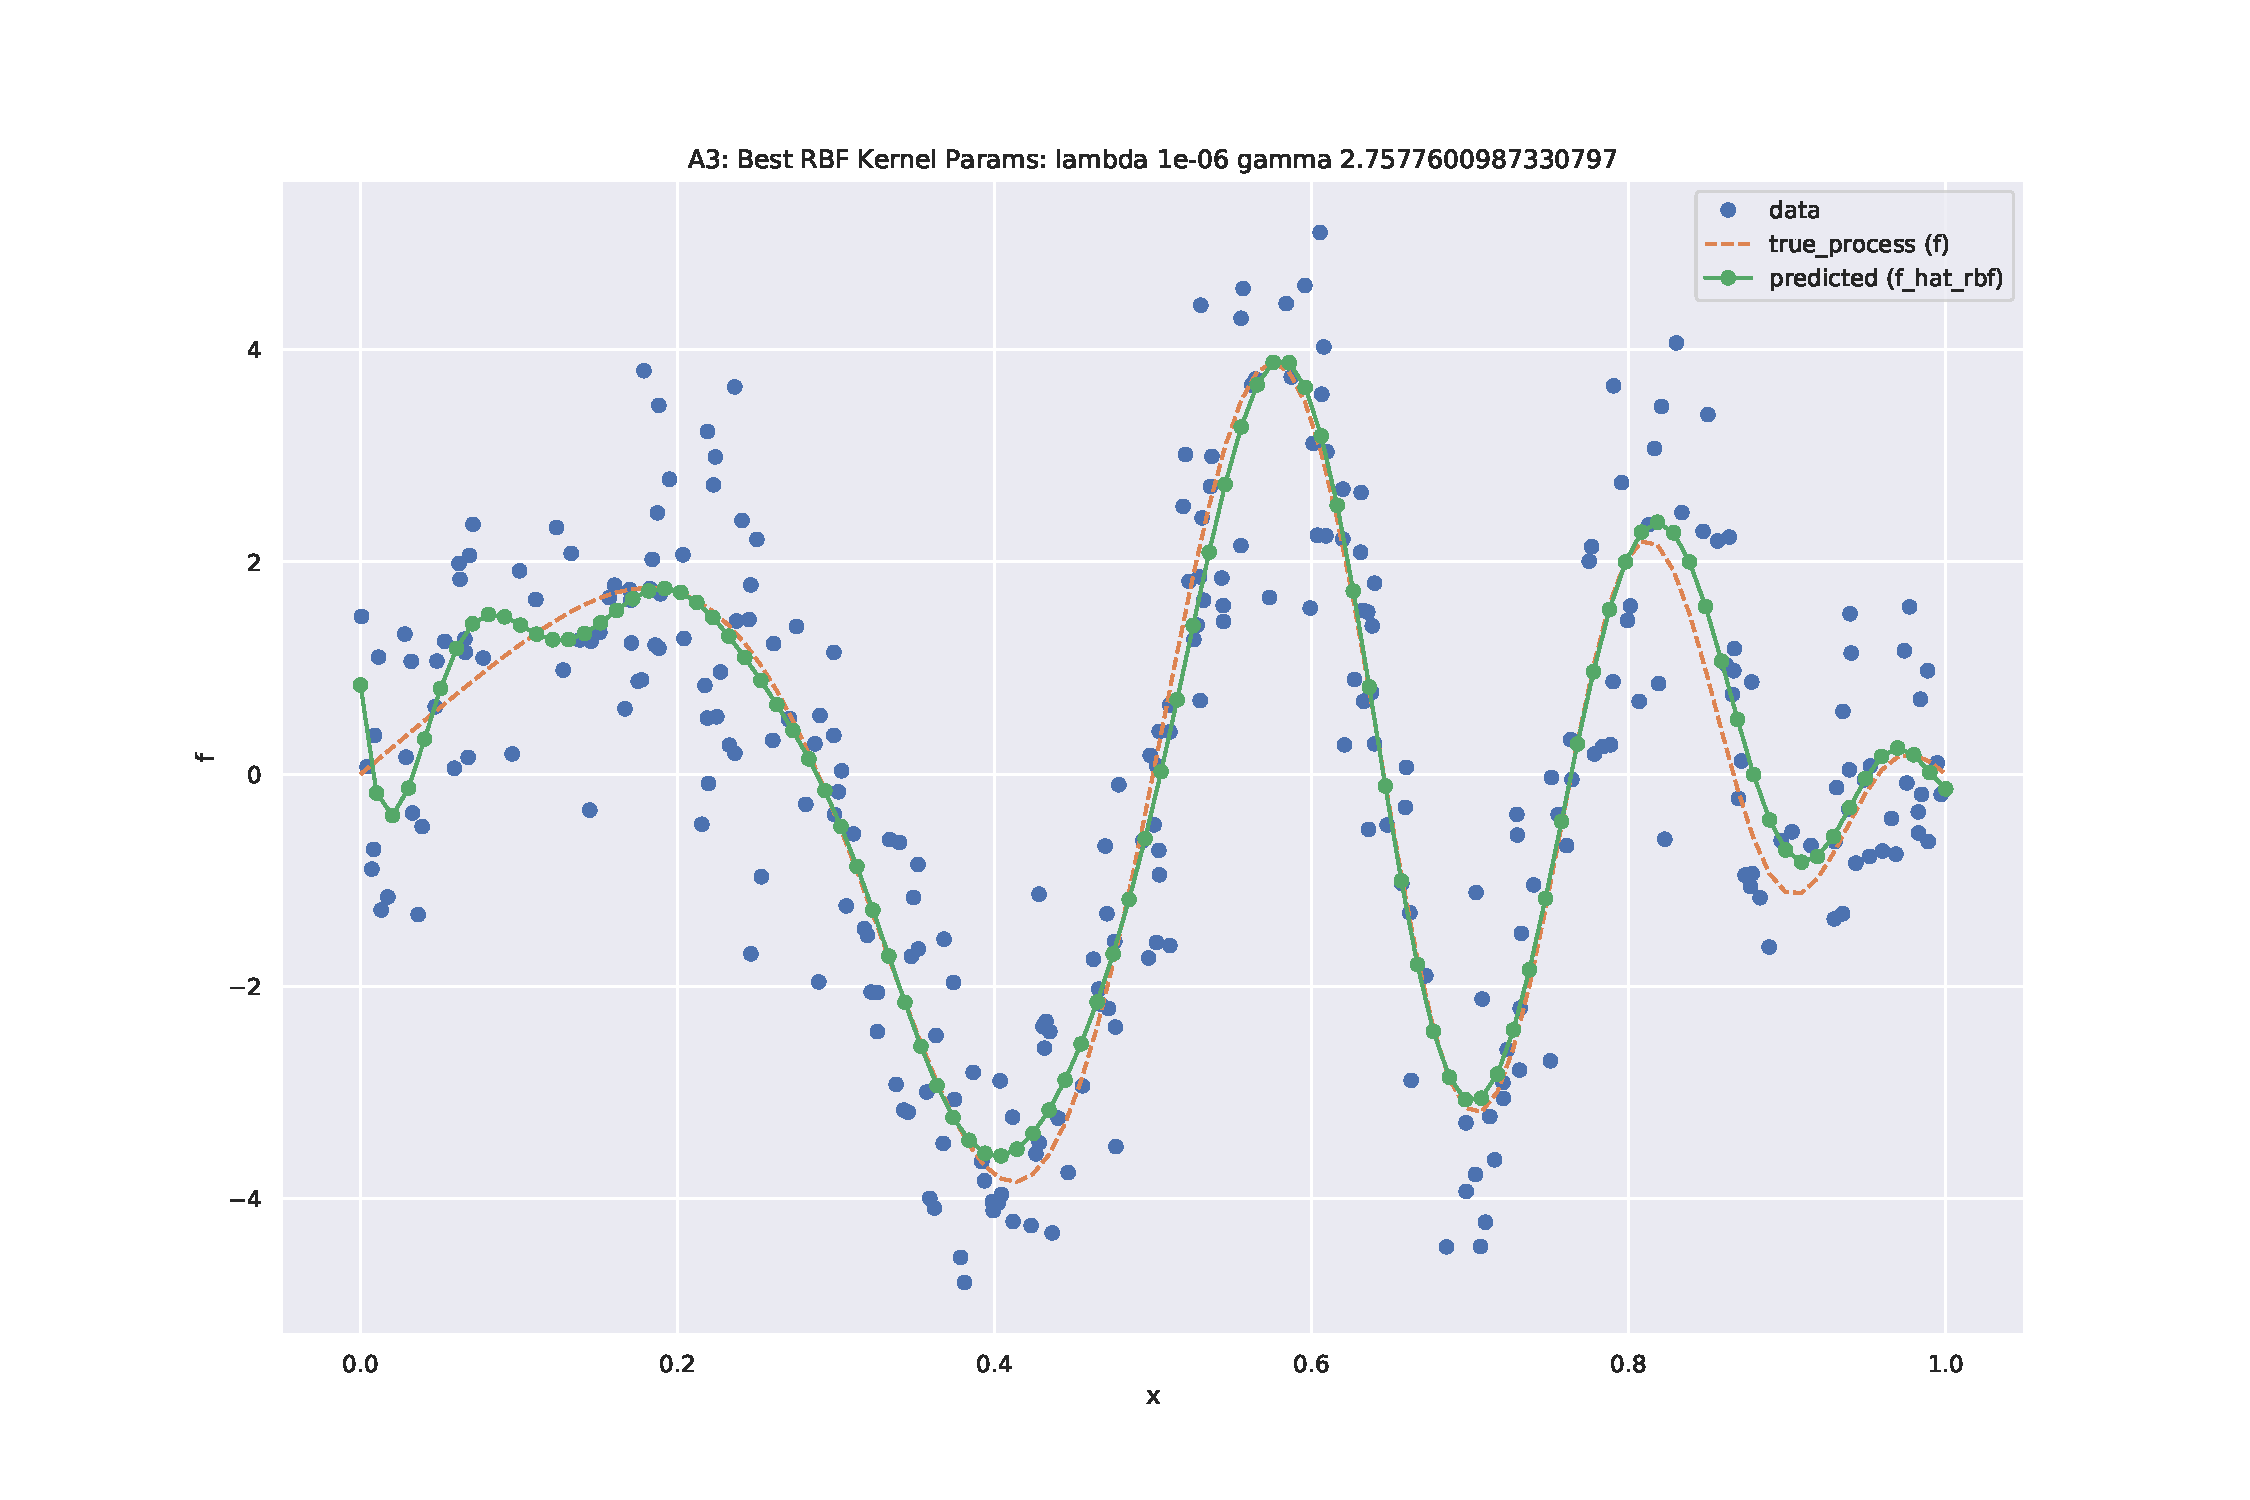
\includegraphics[width=0.49\textwidth]{hw3/code/figures/A3db_rbf.pdf}
            \caption{Problem A3.d Left: Polynomial kernel model, Right: Rbf kernel model}
            \label{figure:a4}
        \end{figure}
        \begin{figure}[h!]
            \centering
            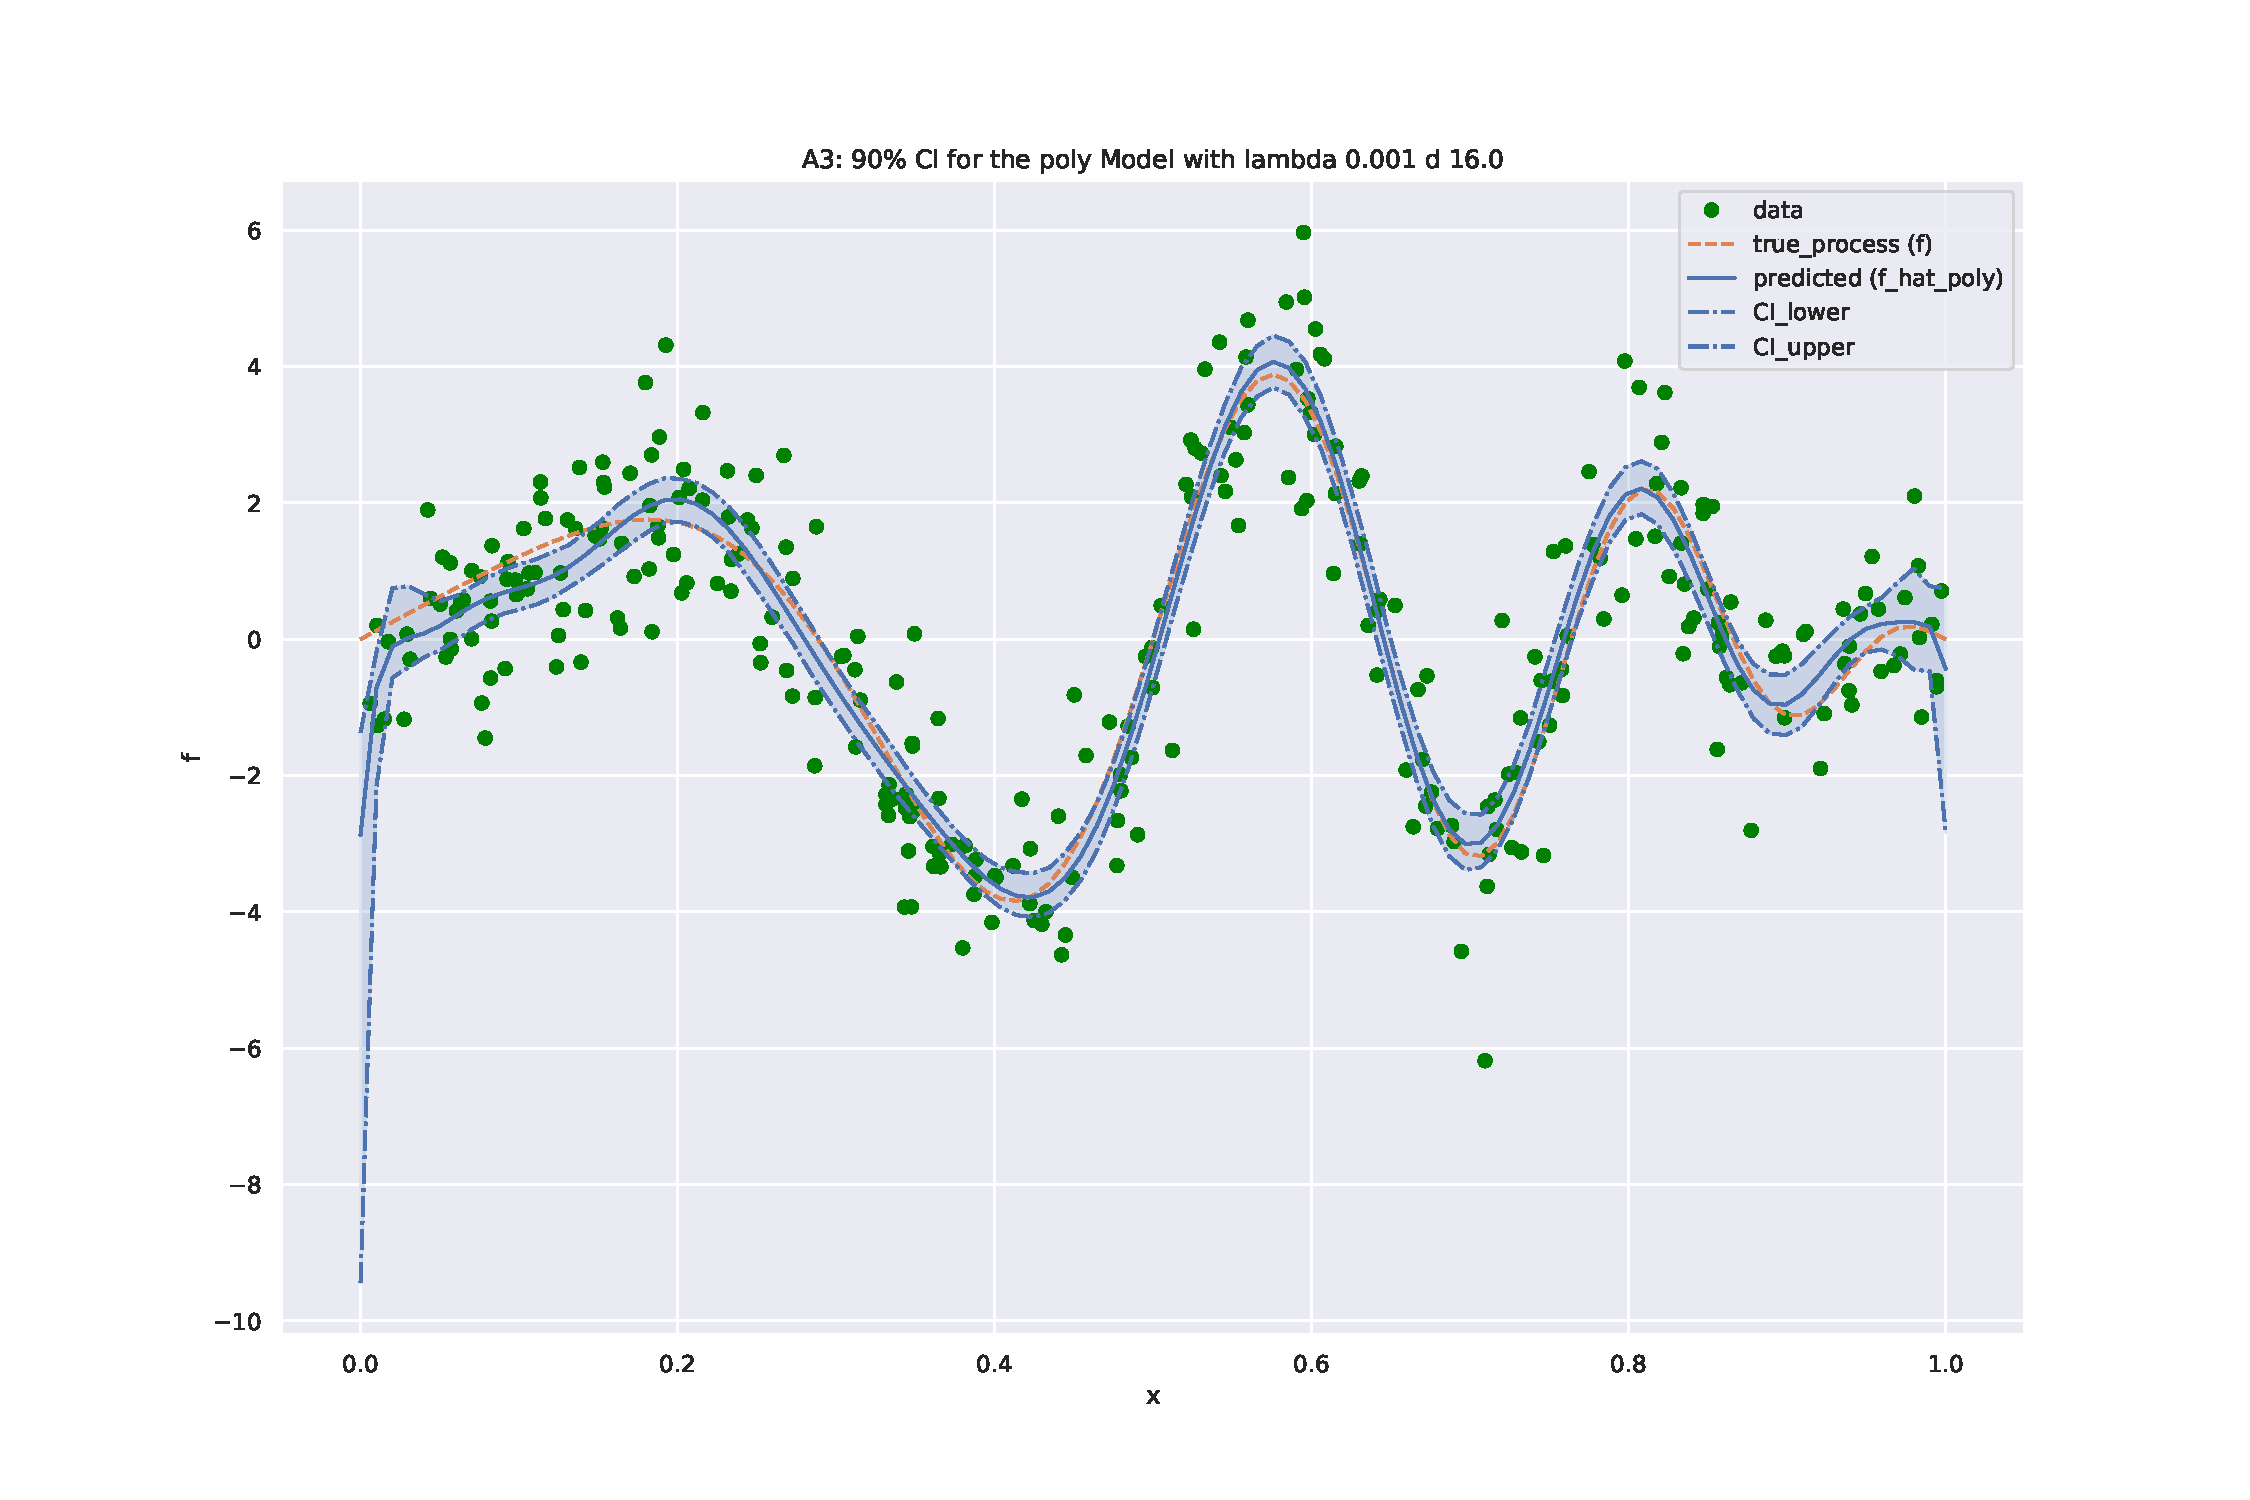
\includegraphics[width=0.49\textwidth]{hw3/code/figures/A3dc_poly.pdf}
            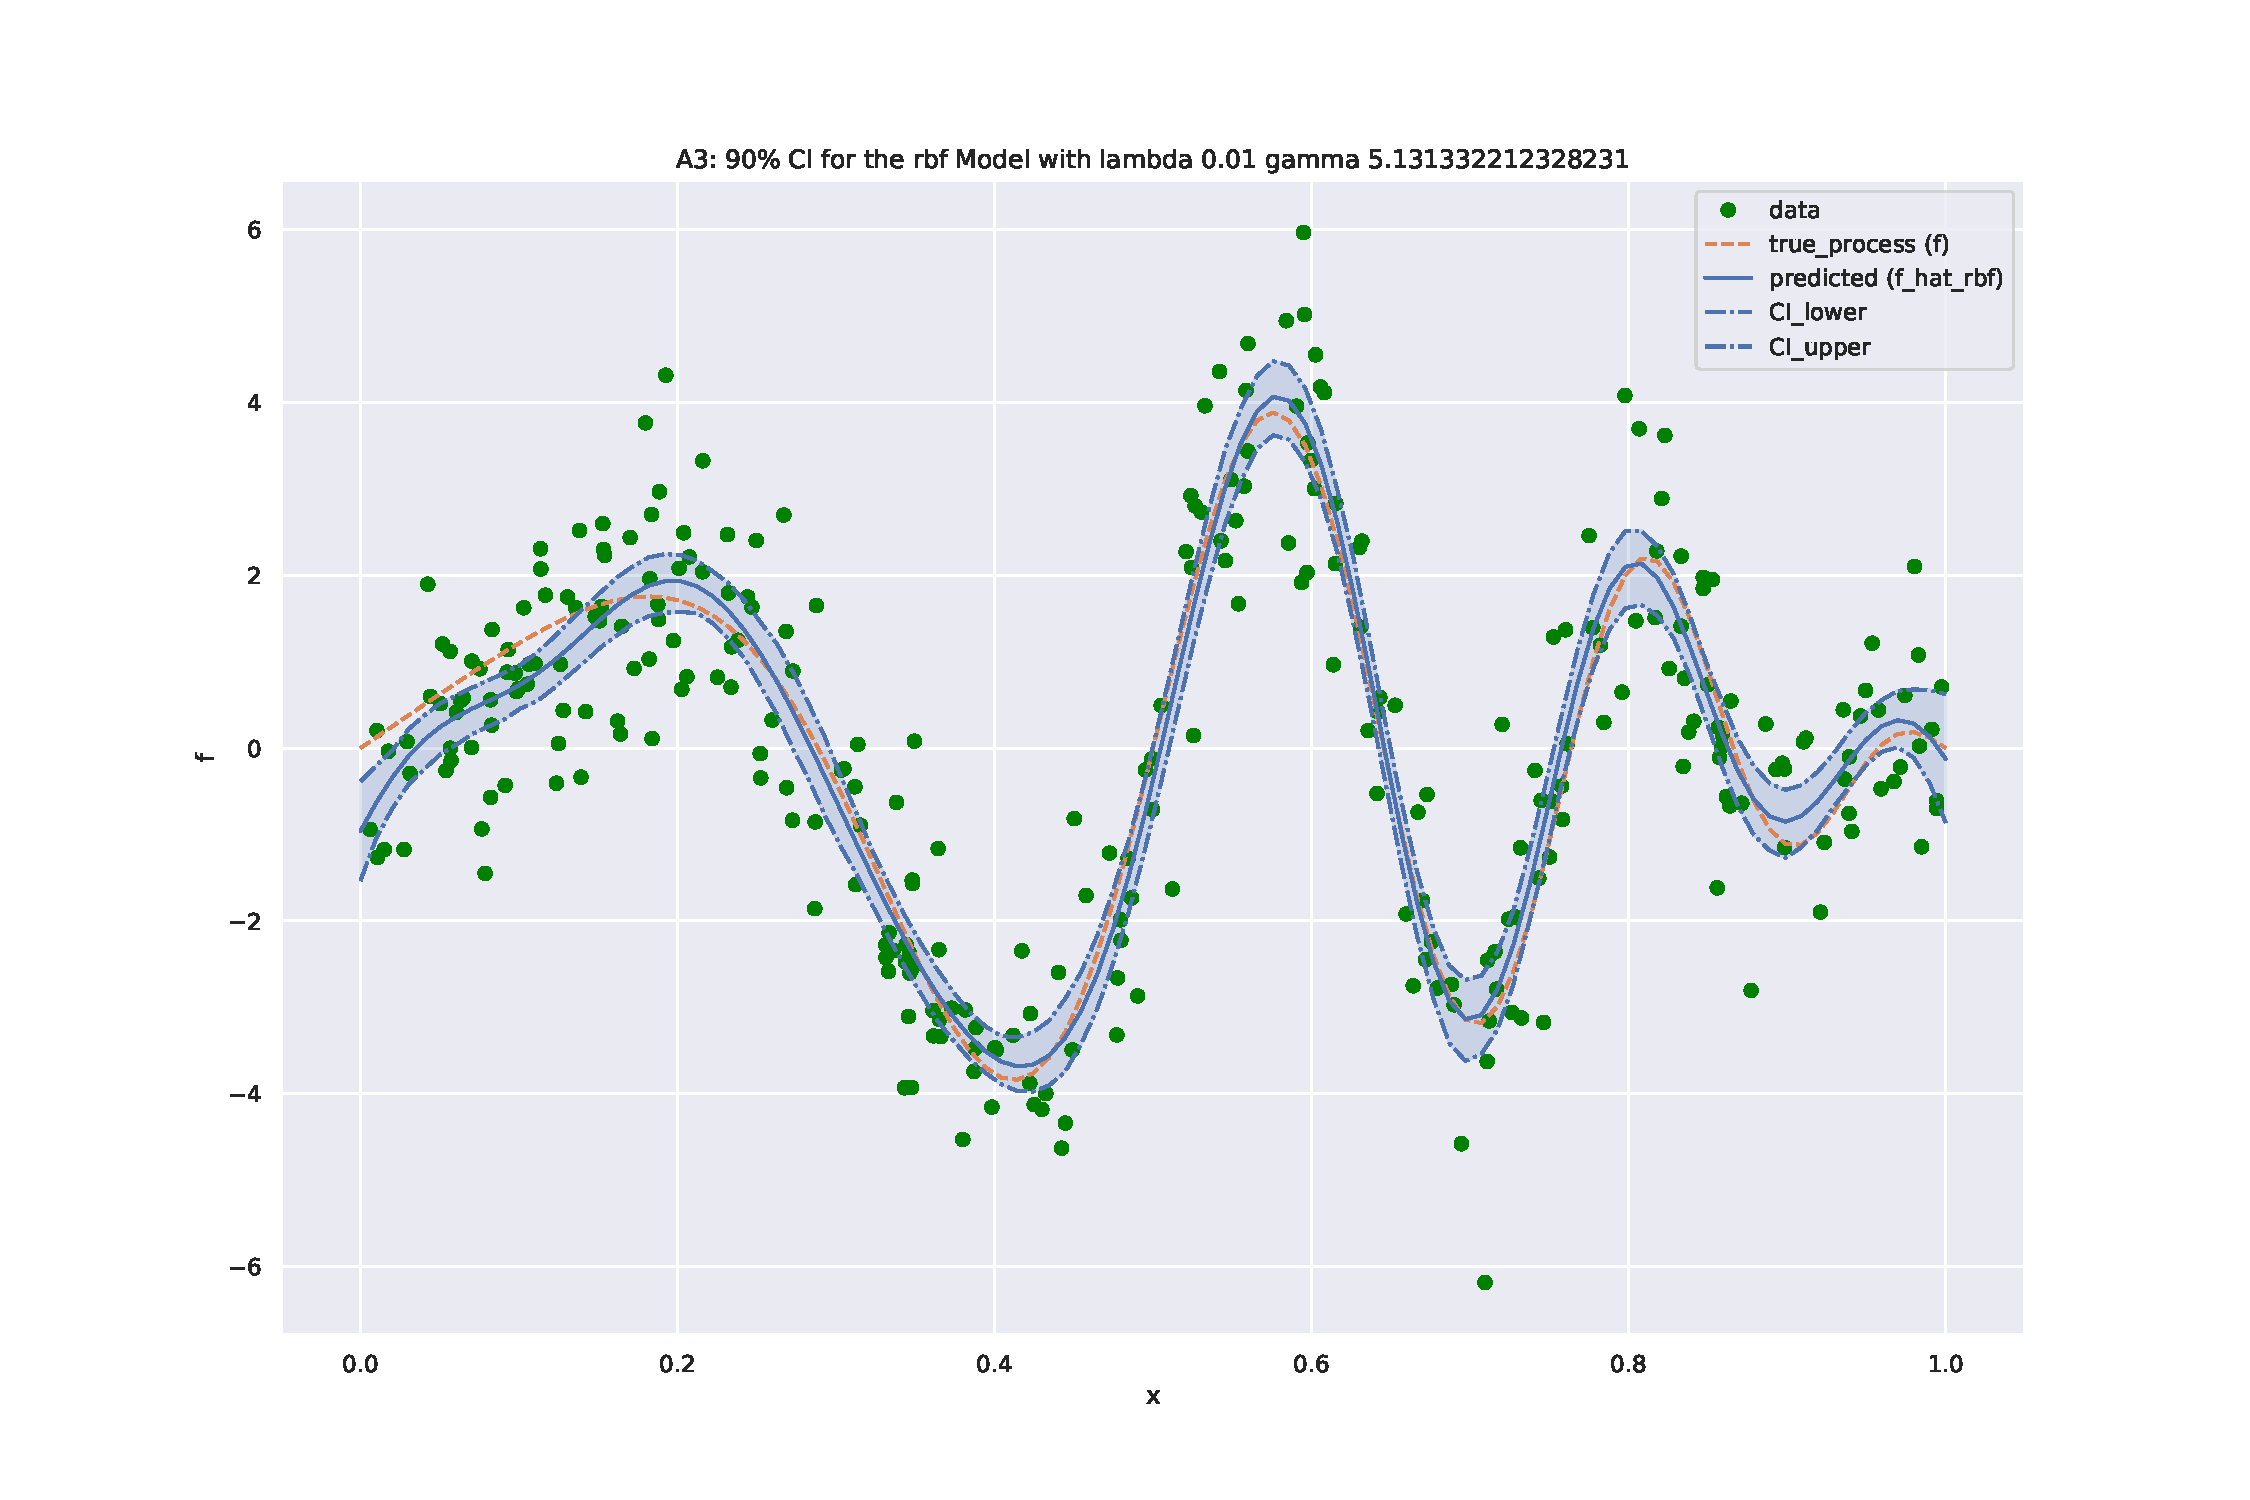
\includegraphics[width=0.49\textwidth]{hw3/code/figures/A3dc_rbf.pdf}
            \caption{Problem A3.d Bootstrap Confidence Intervals. Left: Polynomial kernel model, Right: Rbf kernel model.}
            \label{figure:a4}
        \end{figure}
    \item Expected Squared Error Difference 90\% bootstrap CI: [0.028427236202594672, 0.078246629760424]. We see that zero is not inside this interval which suggests that rbf kernel is better for predicting $Y$ from $X$ since in 90\% of the bootstrap cases, we saw that the rbf kernel model expected error was lower than that of the polynomial kernel model. We also saw above that the polynomial kernel is very unstable.\\
    \\
    See the code for this problem below.
\end{enumerate}  
\newpage
\inputminted{python}{code/A3.py}
\caption{Code for A3}\\
\noindent\rule{\textwidth}{1pt}
\\
\subsection*{k-means clustering}
\noindent\rule{\textwidth}{1pt}
\\
A.4 {\bf Solution:}\\
\begin{enumerate}
    \item \begin{figure}[h!]
            \centering
            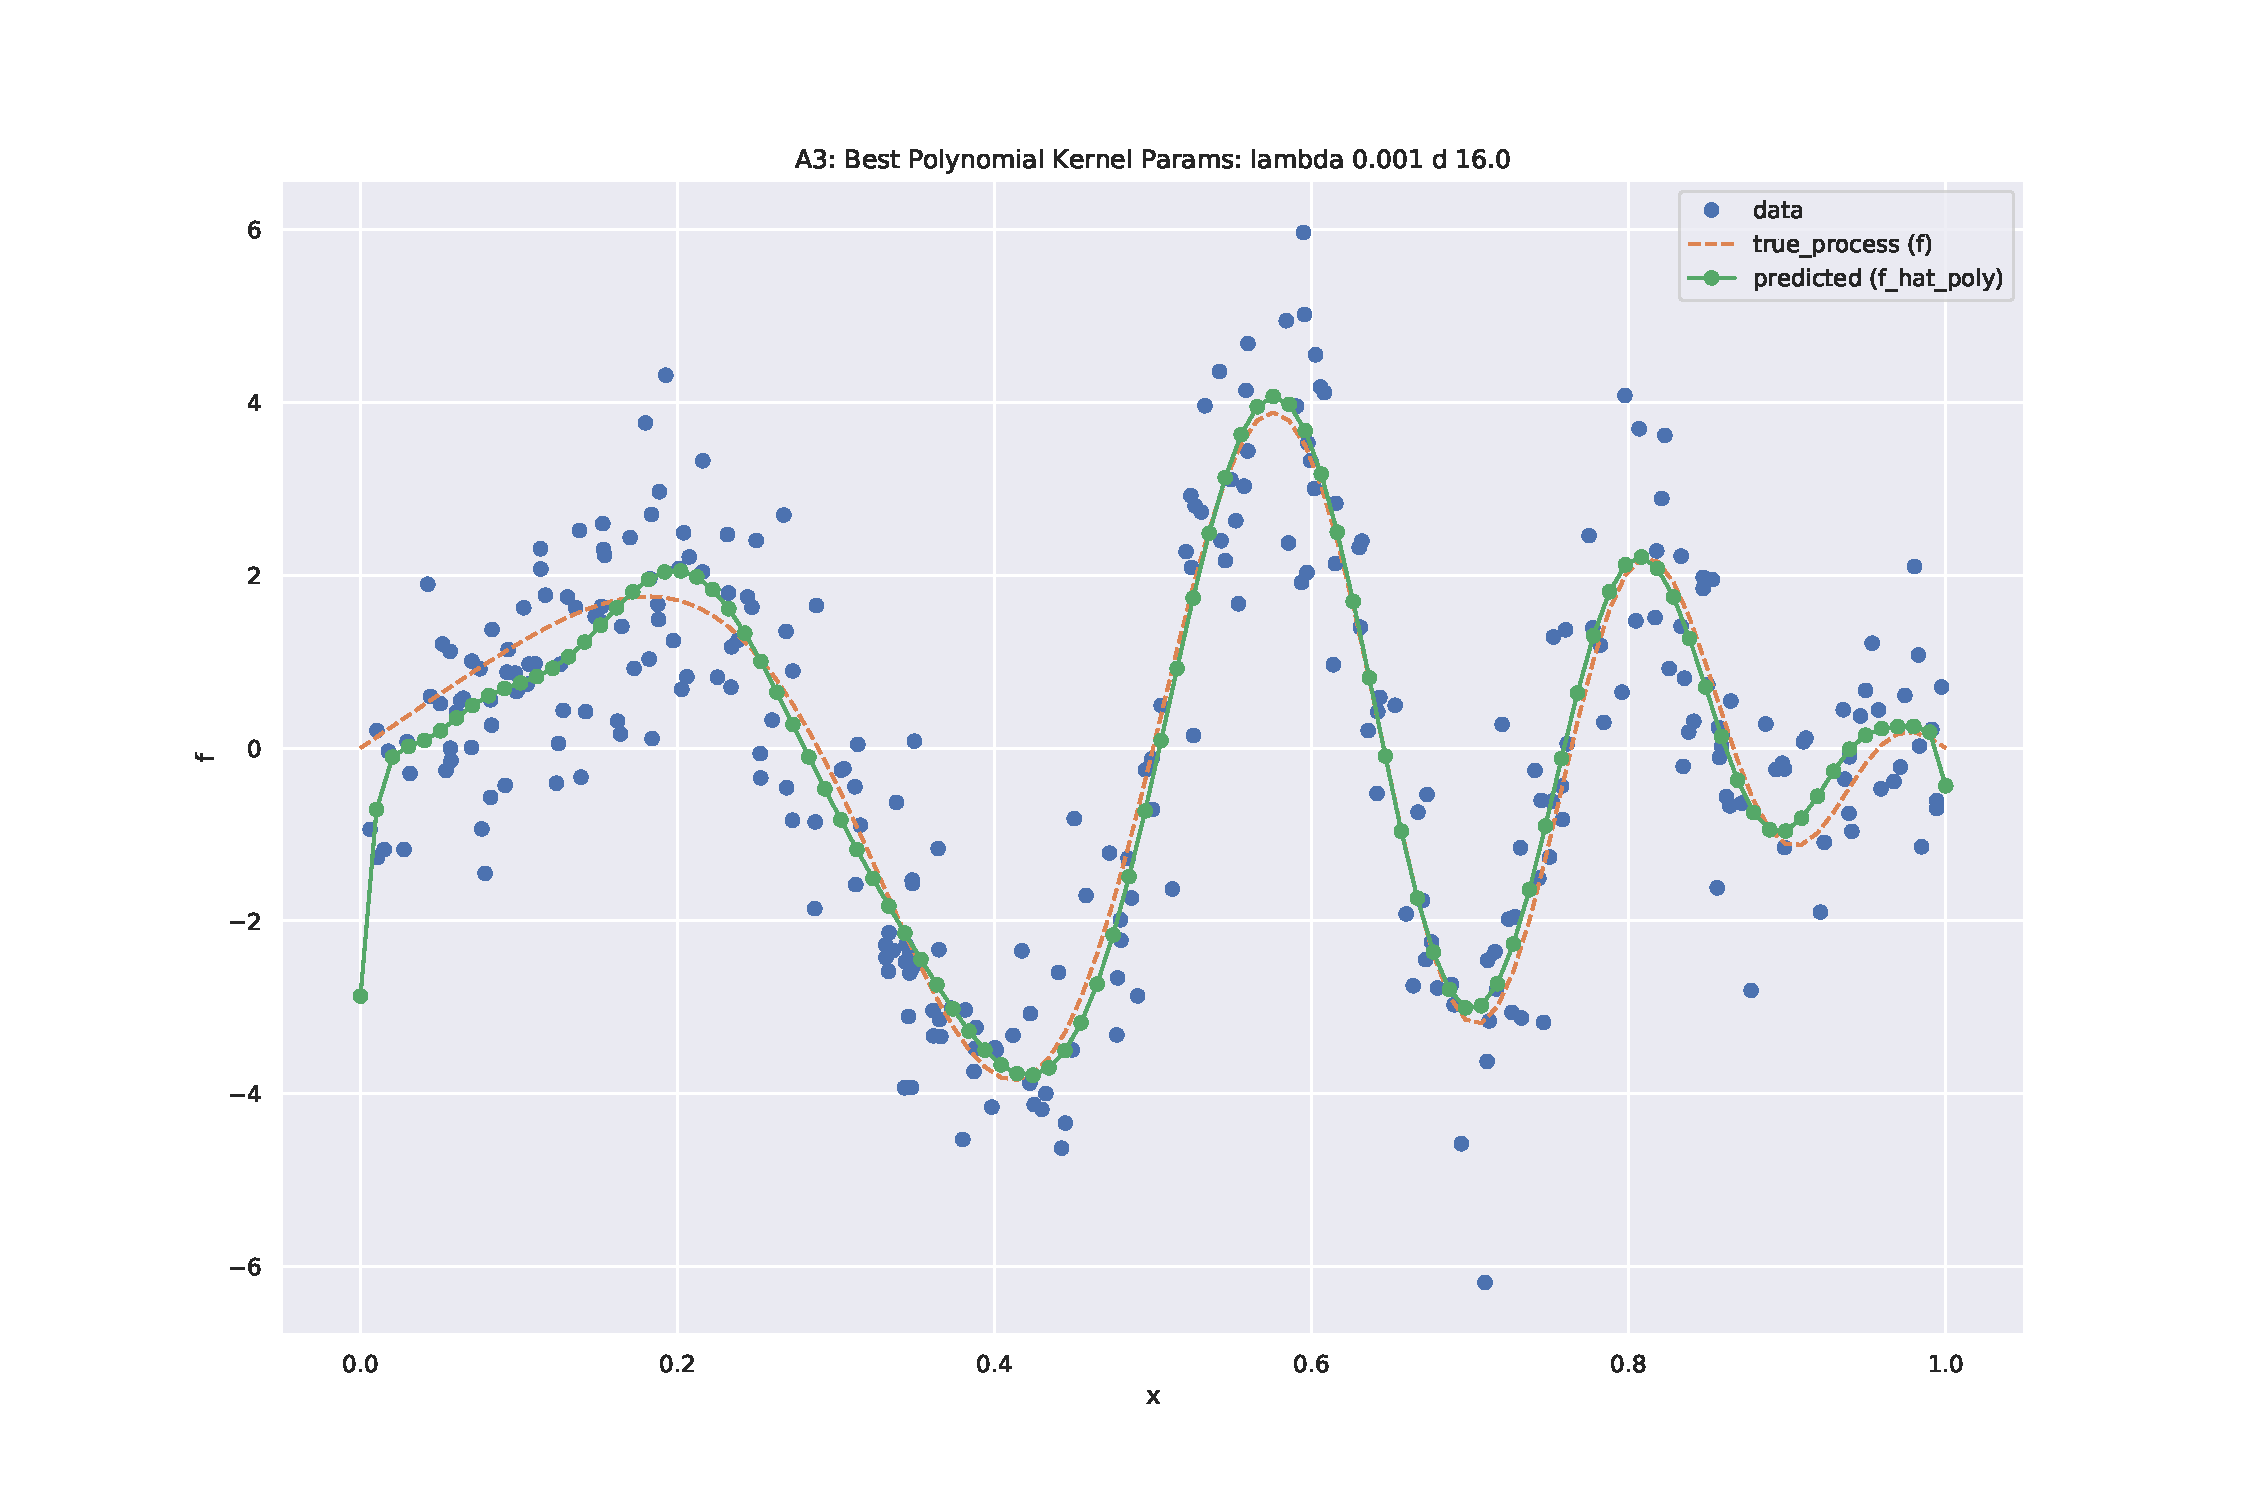
\includegraphics[width=0.49\textwidth]{hw3/code/figures/A3db_poly.pdf}
            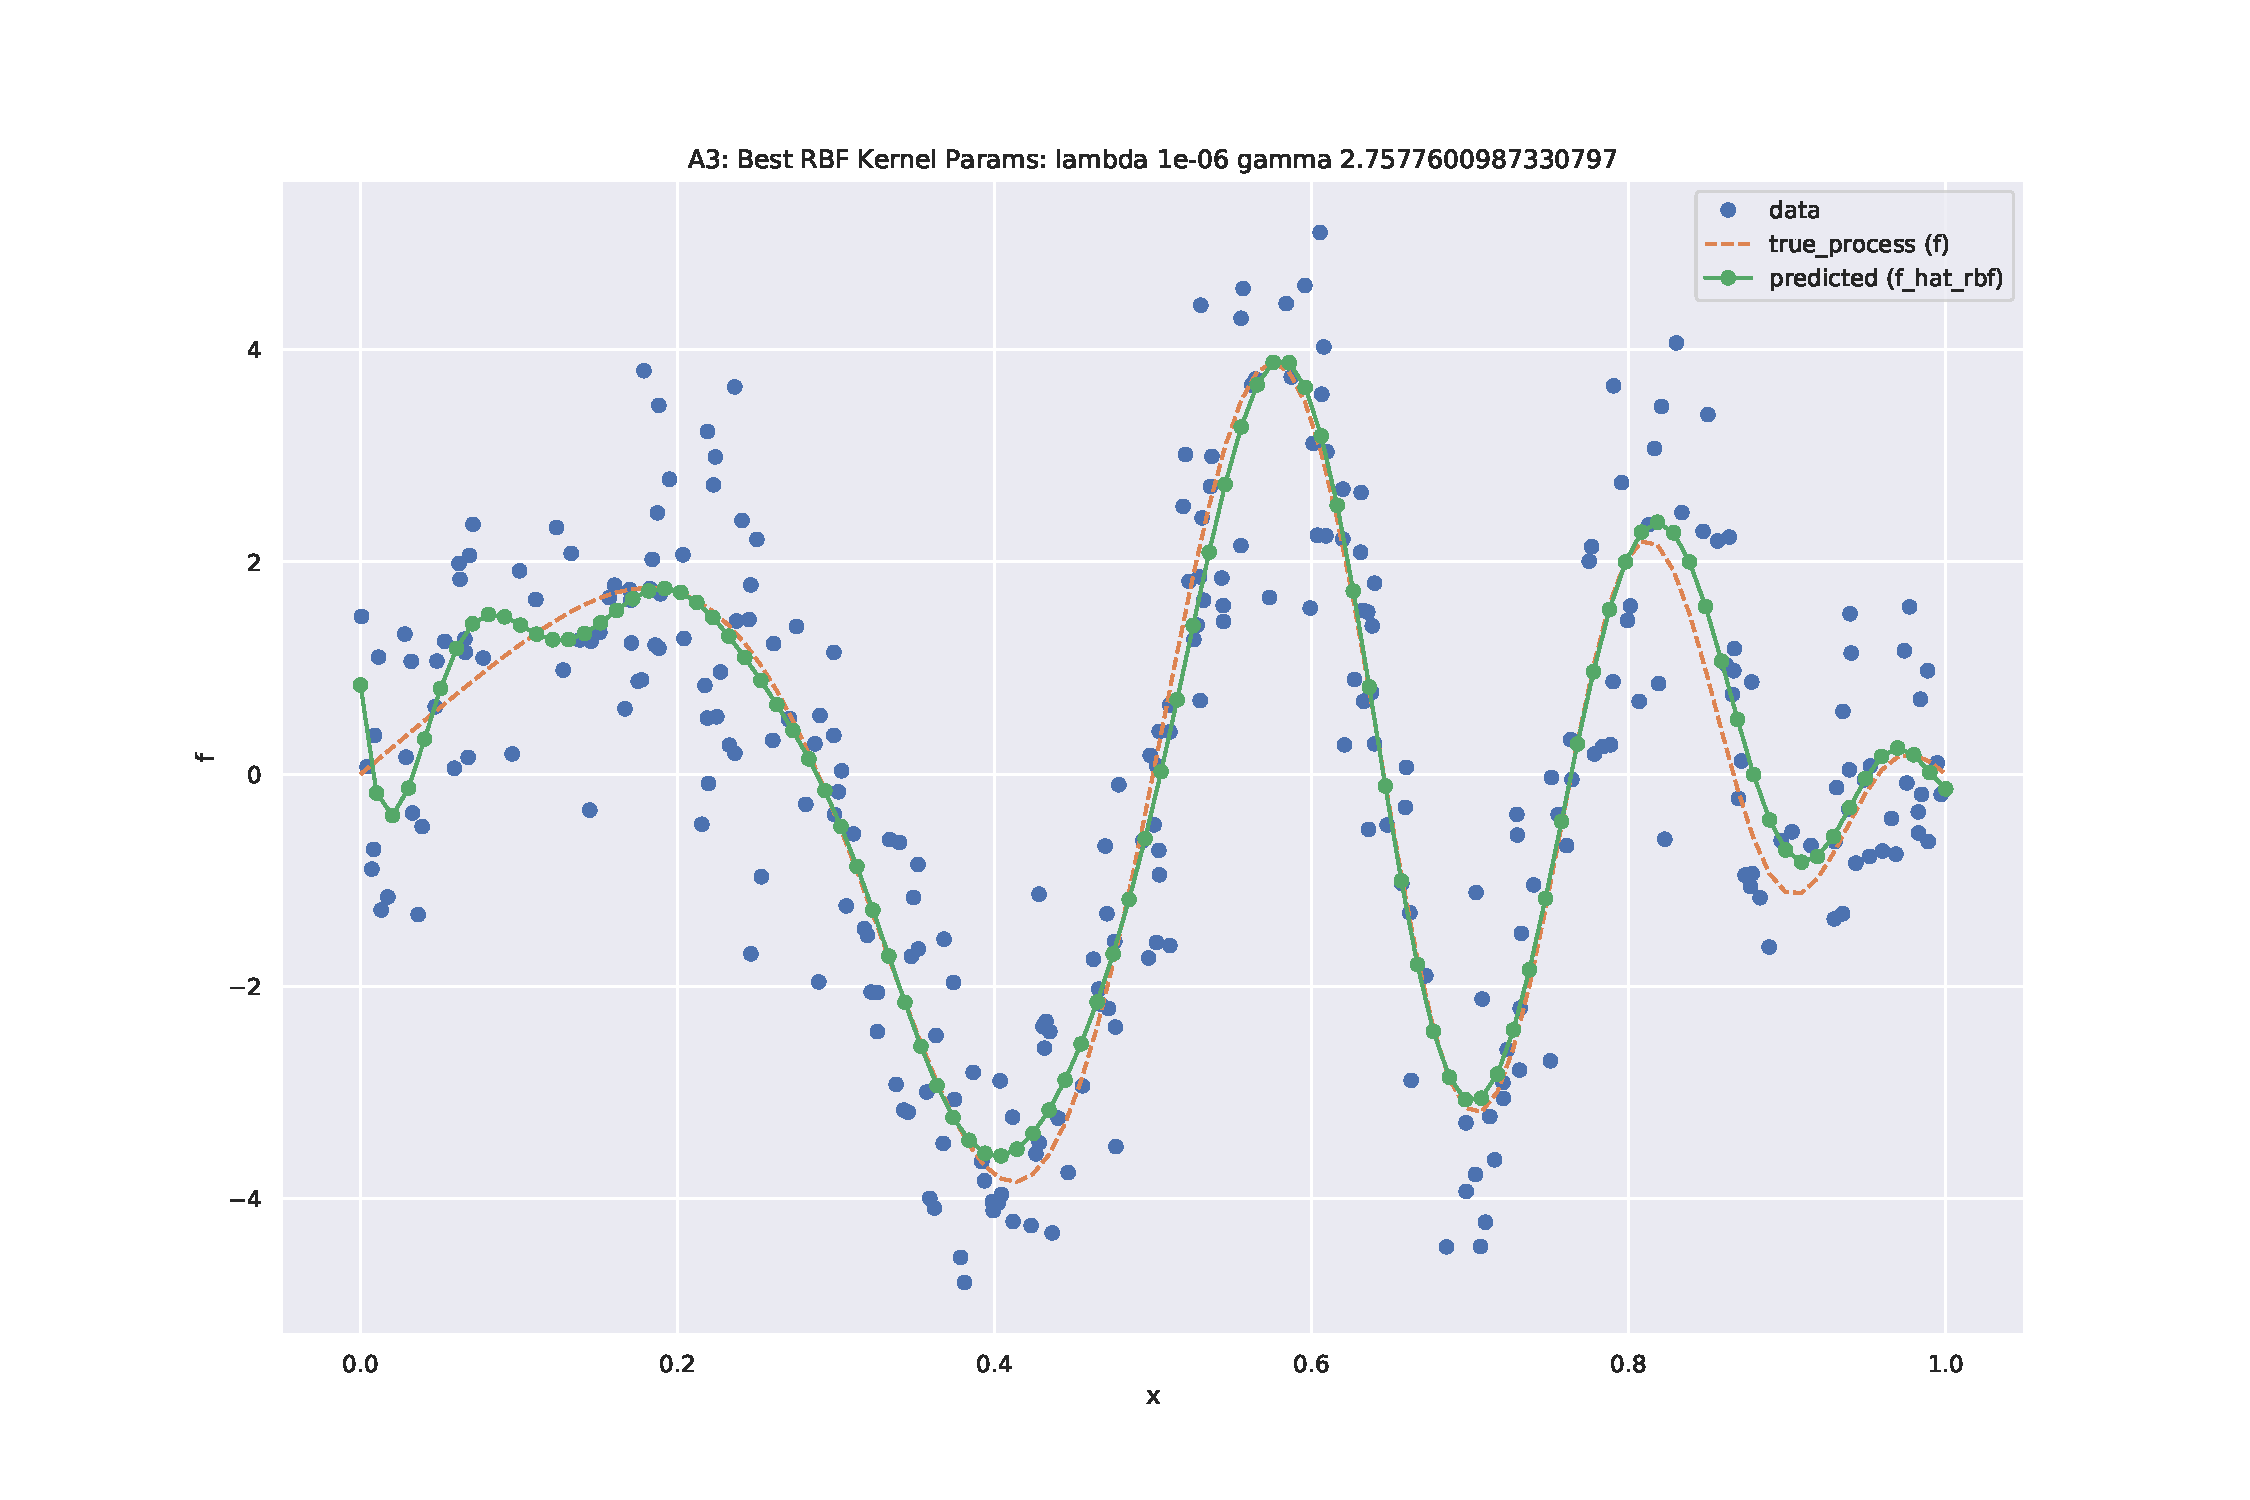
\includegraphics[width=0.49\textwidth]{hw3/code/figures/A3db_rbf.pdf}
            \caption{Problem A3.d Left: Polynomial kernel model, Right: Rbf kernel model}
            \label{figure:a4}
        \end{figure}
\end{enumerate}   
\noindent\rule{\textwidth}{1pt}

\subsection*{Intro to Sample Complexity}
\noindent\rule{\textwidth}{1pt}
\\
B.1 {\bf Solution:}\\
\begin{enumerate}
    \item Using the fact that $R(f) > \epsilon$. Using the definitions and the fact that the expectation of an indicator of an event is the probability of the event and using the fact that samples are iid:
    \begin{align}
    & \P(\hat{R}_n(f) = 0) = \P(\frac{1}{n}\sum_{i=1}^n \I(f(x_i) \not = y_i)) = \P(\forall i: f(x_i) = y_i) = \prod_{i=1}^n \P(f(x_i)=y_i) =  \prod_{i=1}^n (1-\P(f(x_i)\not = y_i)) =  \\
    &= (1-\P(f(x_1)\not = y_1))^n = (1 - \E_{XY}[\I(f(X) \not = Y)])^n = (1 - R(f))^n \le (1-\epsilon)^n \le e^{-n\epsilon} \qquad \Box
    \end{align}
    \item For every $f \in \mathcal{F}$, define $A_f = \{R(f)>\epsilon \text{ and } \hat{R}_n(f) = 0 \}$. Note that $\P(\{R(f)>\epsilon \text{ and } \hat{R}_n(f) = 0 \}) = \P(\hat{R}_n(f) = 0|R(f)>\epsilon)\P(R(f)>\epsilon) \le \P(\hat{R}_n(f) = 0|R(f)>\epsilon)$ and that $\forall f \quad \P(A_f) \le e^{-\epsilon n}$ follows from a. Then:
    $$
    \P(\exists f \in \mathcal{F}: R(f) > \epsilon \text{ and } \hat{R}_n(f) = 0) \le \P(\cup_{f \in \mathcal{F}} A_f) \le \sum_{f \in \mathcal{F}} \P(A_f) \le |\mathcal{F}|e^{-\epsilon n} \qquad \Box
    $$
    \item $$
    |\mathcal{F}|e^{-\epsilon n} \le \delta \Leftrightarrow \epsilon \ge \frac{1}{n}\log \frac{\mathcal{|F|}}{\delta} \Rightarrow \boxed{\epsilon^* = \frac{1}{n}\log \frac{\mathcal{|F|}}{\delta}}
    $$
    \item Note: B1.d is a vaguely worded question. To solve it, let $A$ and $B$ be two boolean events. Then $A \Rightarrow B$ is also a boolean event. Taking into account the truth table for $A \Rightarrow B$, observe $\P(\{A \Rightarrow B \text{ is true}\}) = 1 - \P(\{A \text{ is true}\}  \cap \{B  \text{ is false}\})$. For short,  $\P(A \Rightarrow B) = 1 - \P(A \cap \neg B)$. Now, take $A = \{\hat{R}_n(f) = 0\}$ and $B = \{R(f) - R(f^*) \le \frac{1}{n}\log \frac{\mathcal{|F|}}{\delta}\} =c $ (omitting hats over $f$ for brevity since any function with zero empirical risk automatically becomes its argmin, since the empirical risk is non-negative). Finally, for $A$ and $B$ defined above (and since $R(f^*) \ge 0$) and using previous parts:
    \begin{align}
        &\P(A \Rightarrow B) = 1 - \P(A \cap \neg B) = 1 - \P(\hat{R}_n(f) = 0 \text{ and } R(f) - R(f^*) > \epsilon^*) \ge \\
        & \ge 1 - \P(\hat{R}_n(f) = 0 \text{ and } R(f) > \epsilon^*) \ge
        1 - \P(\exists f \in \mathcal{F}: R(f) > \epsilon^* \text{ and } \hat{R}_n(f) = 0) \ge \\
        &\ge 1 - |\mathcal{F}|e^{-\epsilon^* n} \ge 1 - \delta \qquad \Box
    \end{align}
    \end{enumerate}   
\noindent\rule{\textwidth}{1pt}

\noindent\rule{\textwidth}{1pt}
\\
B.3 {\bf Solution:}\\
\begin{enumerate}
    \item 
    \begin{itemize}
        \item  Let's first show that the sum of convex functions is convex. Let $f,g$ be convex, consider $f(x) + g(x)$. Take any $\lambda \in [0,1]$, take any $x, y$. Then, by convexity of $f$ and $g$:
        $$
        f(\lambda x + (1-\lambda)y) + g(\lambda x + (1-\lambda)y) \le \lambda f(x) + (1-\lambda)f(y) + \lambda g(x) + (1-\lambda)g(y) = \lambda (f(x) + g(x)) + (1-\lambda)(f(y) + g(y)). \Box
        $$
        That is, $f(x) + g(x)$ is convex if $f(x)$ and $g(x)$ are convex. Now, a sum $\sum_{i=1}^n f_i(x)$ of $n$ convex functions $f_i(x)$ is also convex because by the above we can first show that $f_1(x) + f_2(x)$ is convex, that implies the convexity of $f_1(x) + f_2(x) + f_3(x)$, etc. At every step $j$, we know that $\sum_{i=1}^{j}f_i(x)$ is convex and $f_{j+1}(x)$ is also convex, so $\sum_{i=1}^{j+1}f_i(x)$ is convex. That is, by induction, it follows that $\sum_{i=1}^n f_i(x)$ is convex. $\Box$
        \item Now, multiplication by $\lambda > 0$ obviously preserves convexity and thus $\lambda\|w\|$ is convex because $\|w\|$ is convex. To see that, take any $\alpha \in [0,1]$ and any $x,y$:
        $$
        \lambda\|\alpha x + (1-\alpha)y\| \le \lambda(\alpha\|x\| + (1-\alpha)\|y\|) = \alpha\lambda\|x\| + (1-\alpha)\lambda\|y\|
        $$
        \item Finally, since $l_i(w) \text{ are convex } \Rightarrow \sum_{i=1}^n l_i(w)$ is convex. As shown above, $\lambda \|w\|$ is convex too. So 
        $\sum_{i=1}^n l_i(w) + \lambda \|w\|$ is convex as a sum of two convex functions. $\Box$
    \end{itemize}
    \item Because convexity implies that every local minimum is a global minimum. $\Box$
\end{enumerate}   
\noindent\rule{\textwidth}{1pt}


\subsection*{Lasso}

\noindent\rule{\textwidth}{1pt}
A.4 {\bf Solution:}\\
\begin{enumerate}
    \item See Plot 1 in Figure 2 (left). Note that for this problem I treated numbers less than 1e-14 in absolute value as zeros.
    \item See Plot 2 in Figure 2 (right). 
        \begin{figure}[h!]
            \centering
            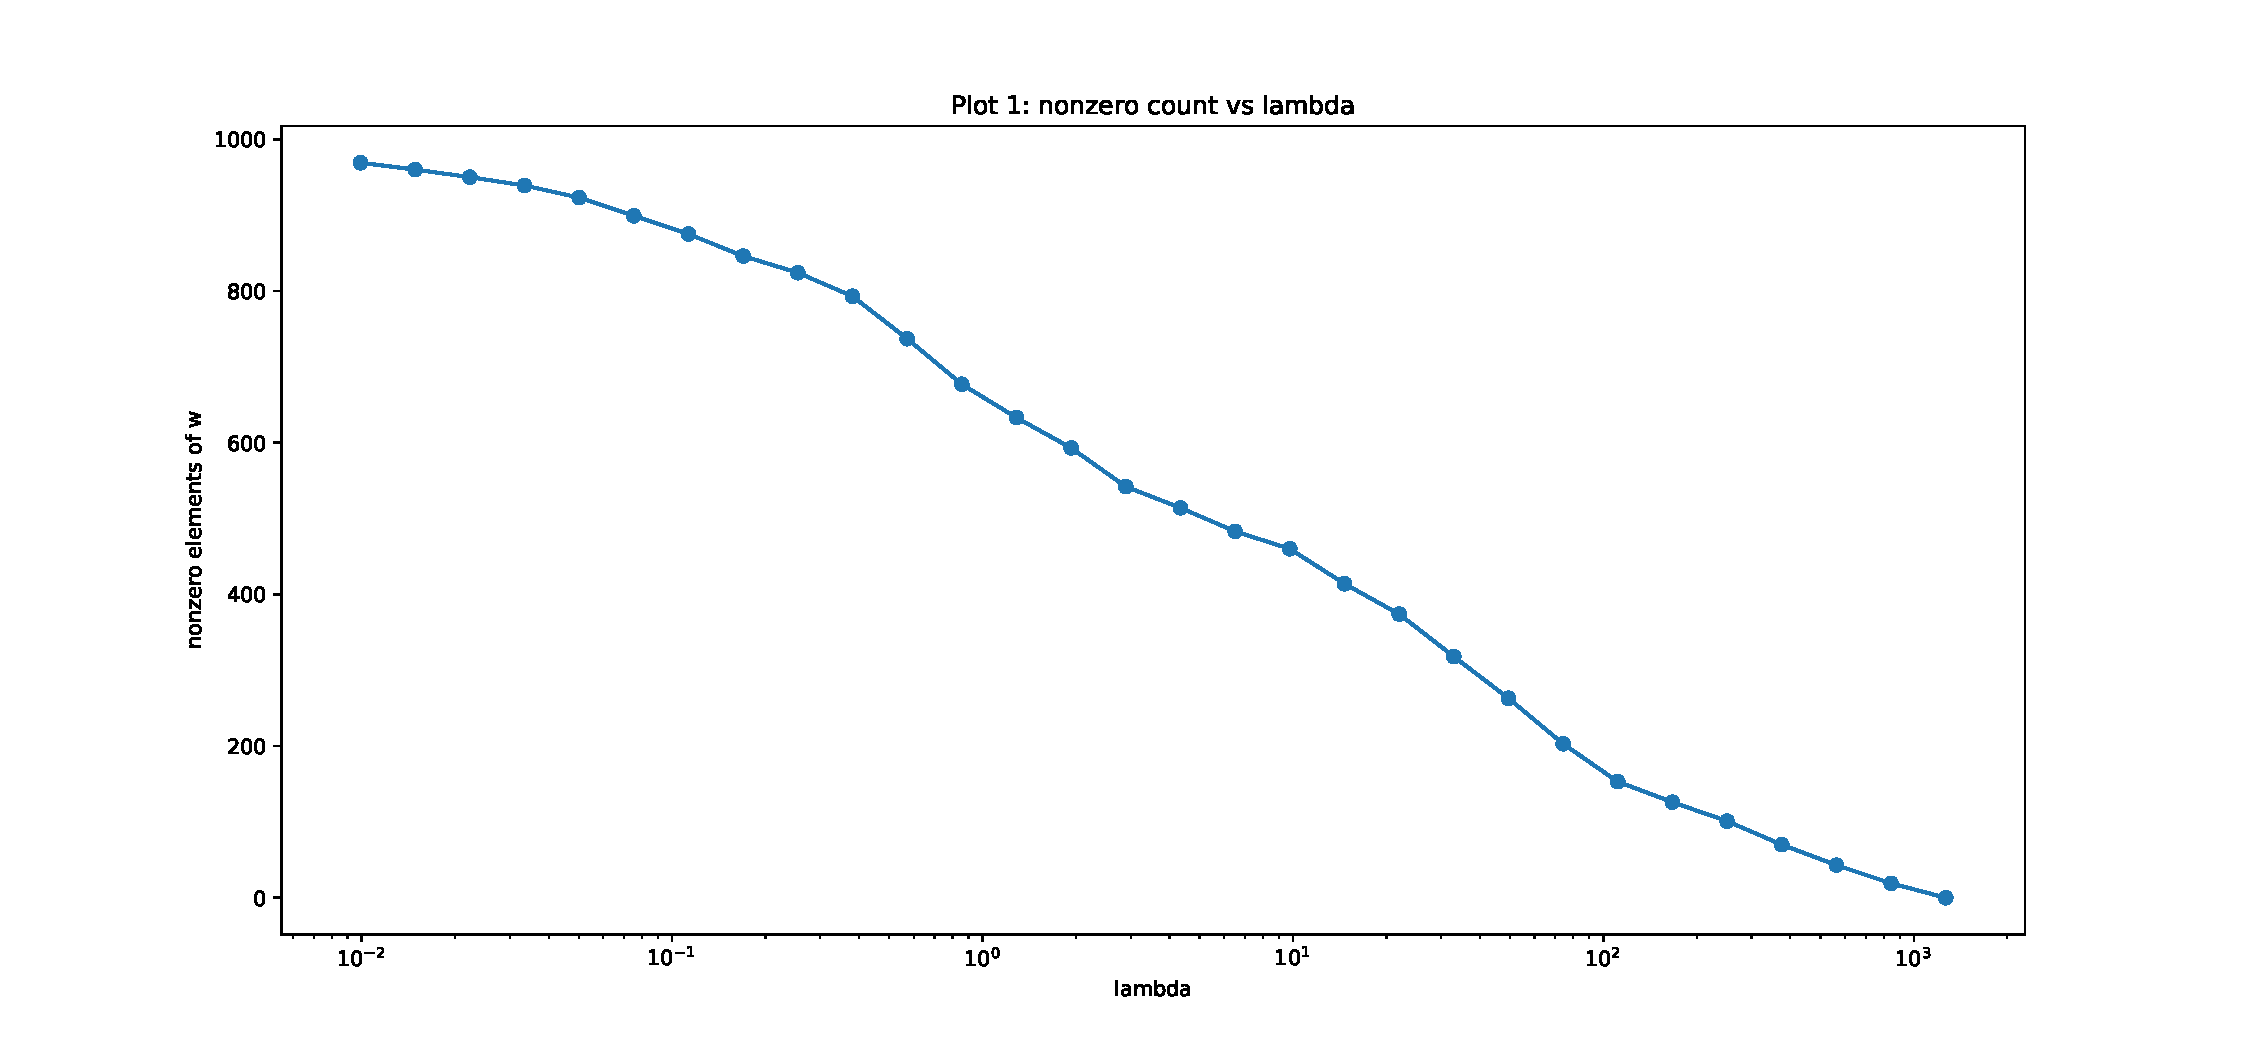
\includegraphics[width=0.45\textwidth]{hw2/code/figures/A4a.pdf}
            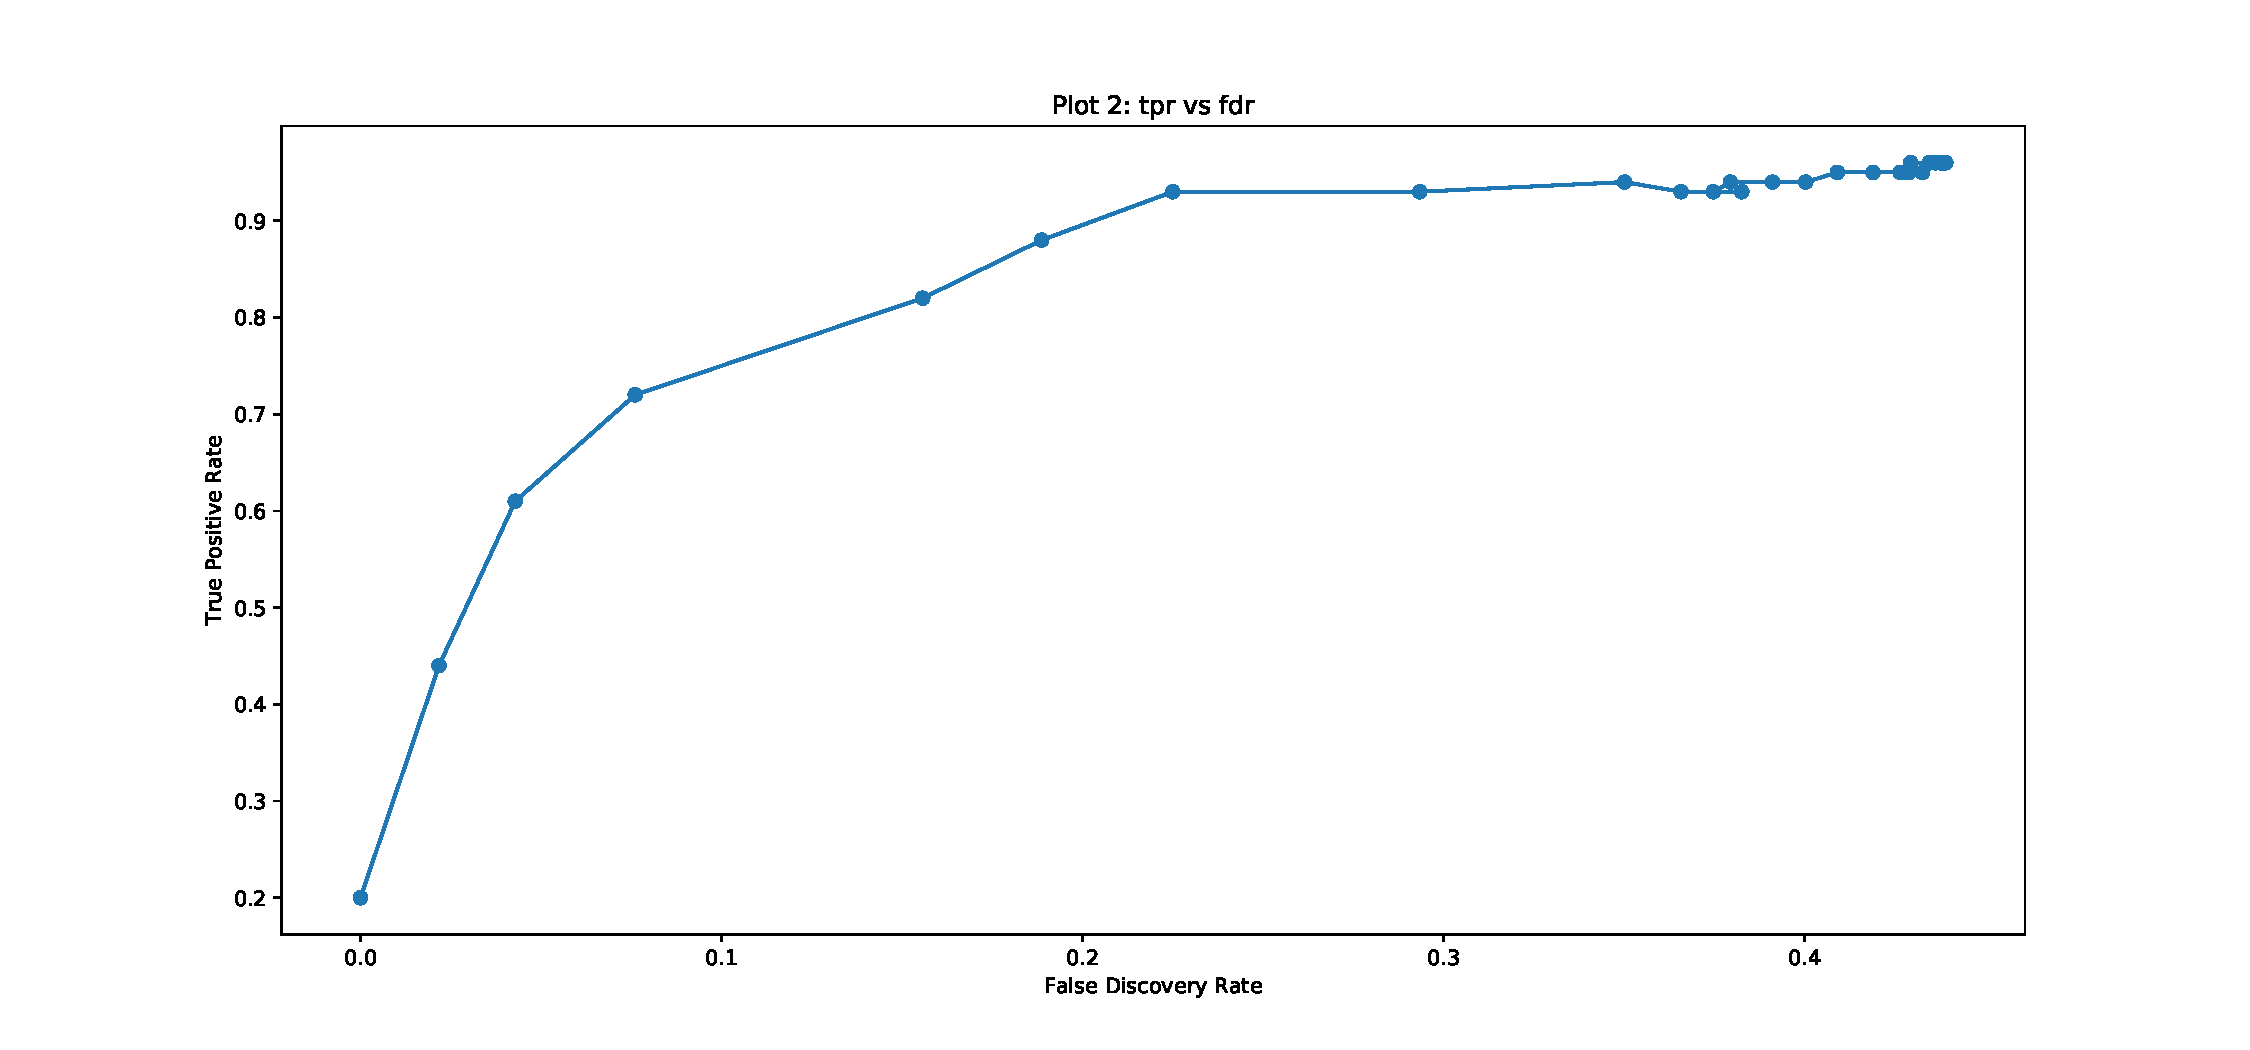
\includegraphics[width=0.45\textwidth]{hw2/code/figures/A4b.pdf}
            \caption{Problem A4. Left: A4.a, Right: A4.b}
            \label{figure:a4}
        \end{figure}
    \item From the plots we see, as expected, that greater $\lambda$ forces more weights to zero. That is, increasing $\lambda$ results in a more sparse solution. However, in Plot 2, we see that too large $\lambda$ results in zero solution which gives poor performance. If we use $\lambda$ which is too small, we end up in another extreme, where we have a high false discovery rate. One should choose $\lambda$ which is close to the upper left corner on Plot 2. (Probably, making this plot on a validation set would be a good idea too for choosing $\lambda$).
\end{enumerate}
\inputminted{python}{code/A4.py}
\caption{Code for A4}
\noindent\rule{\textwidth}{1pt}



\noindent\rule{\textwidth}{1pt}
A.5 {\bf Solution:}\\
\begin{enumerate}
    \item See Figure 3 (top left). 
    \item See Figure 3 (top right). 
    \item See Figure 3 (bottom).
        \begin{figure}[h!]
            \centering
            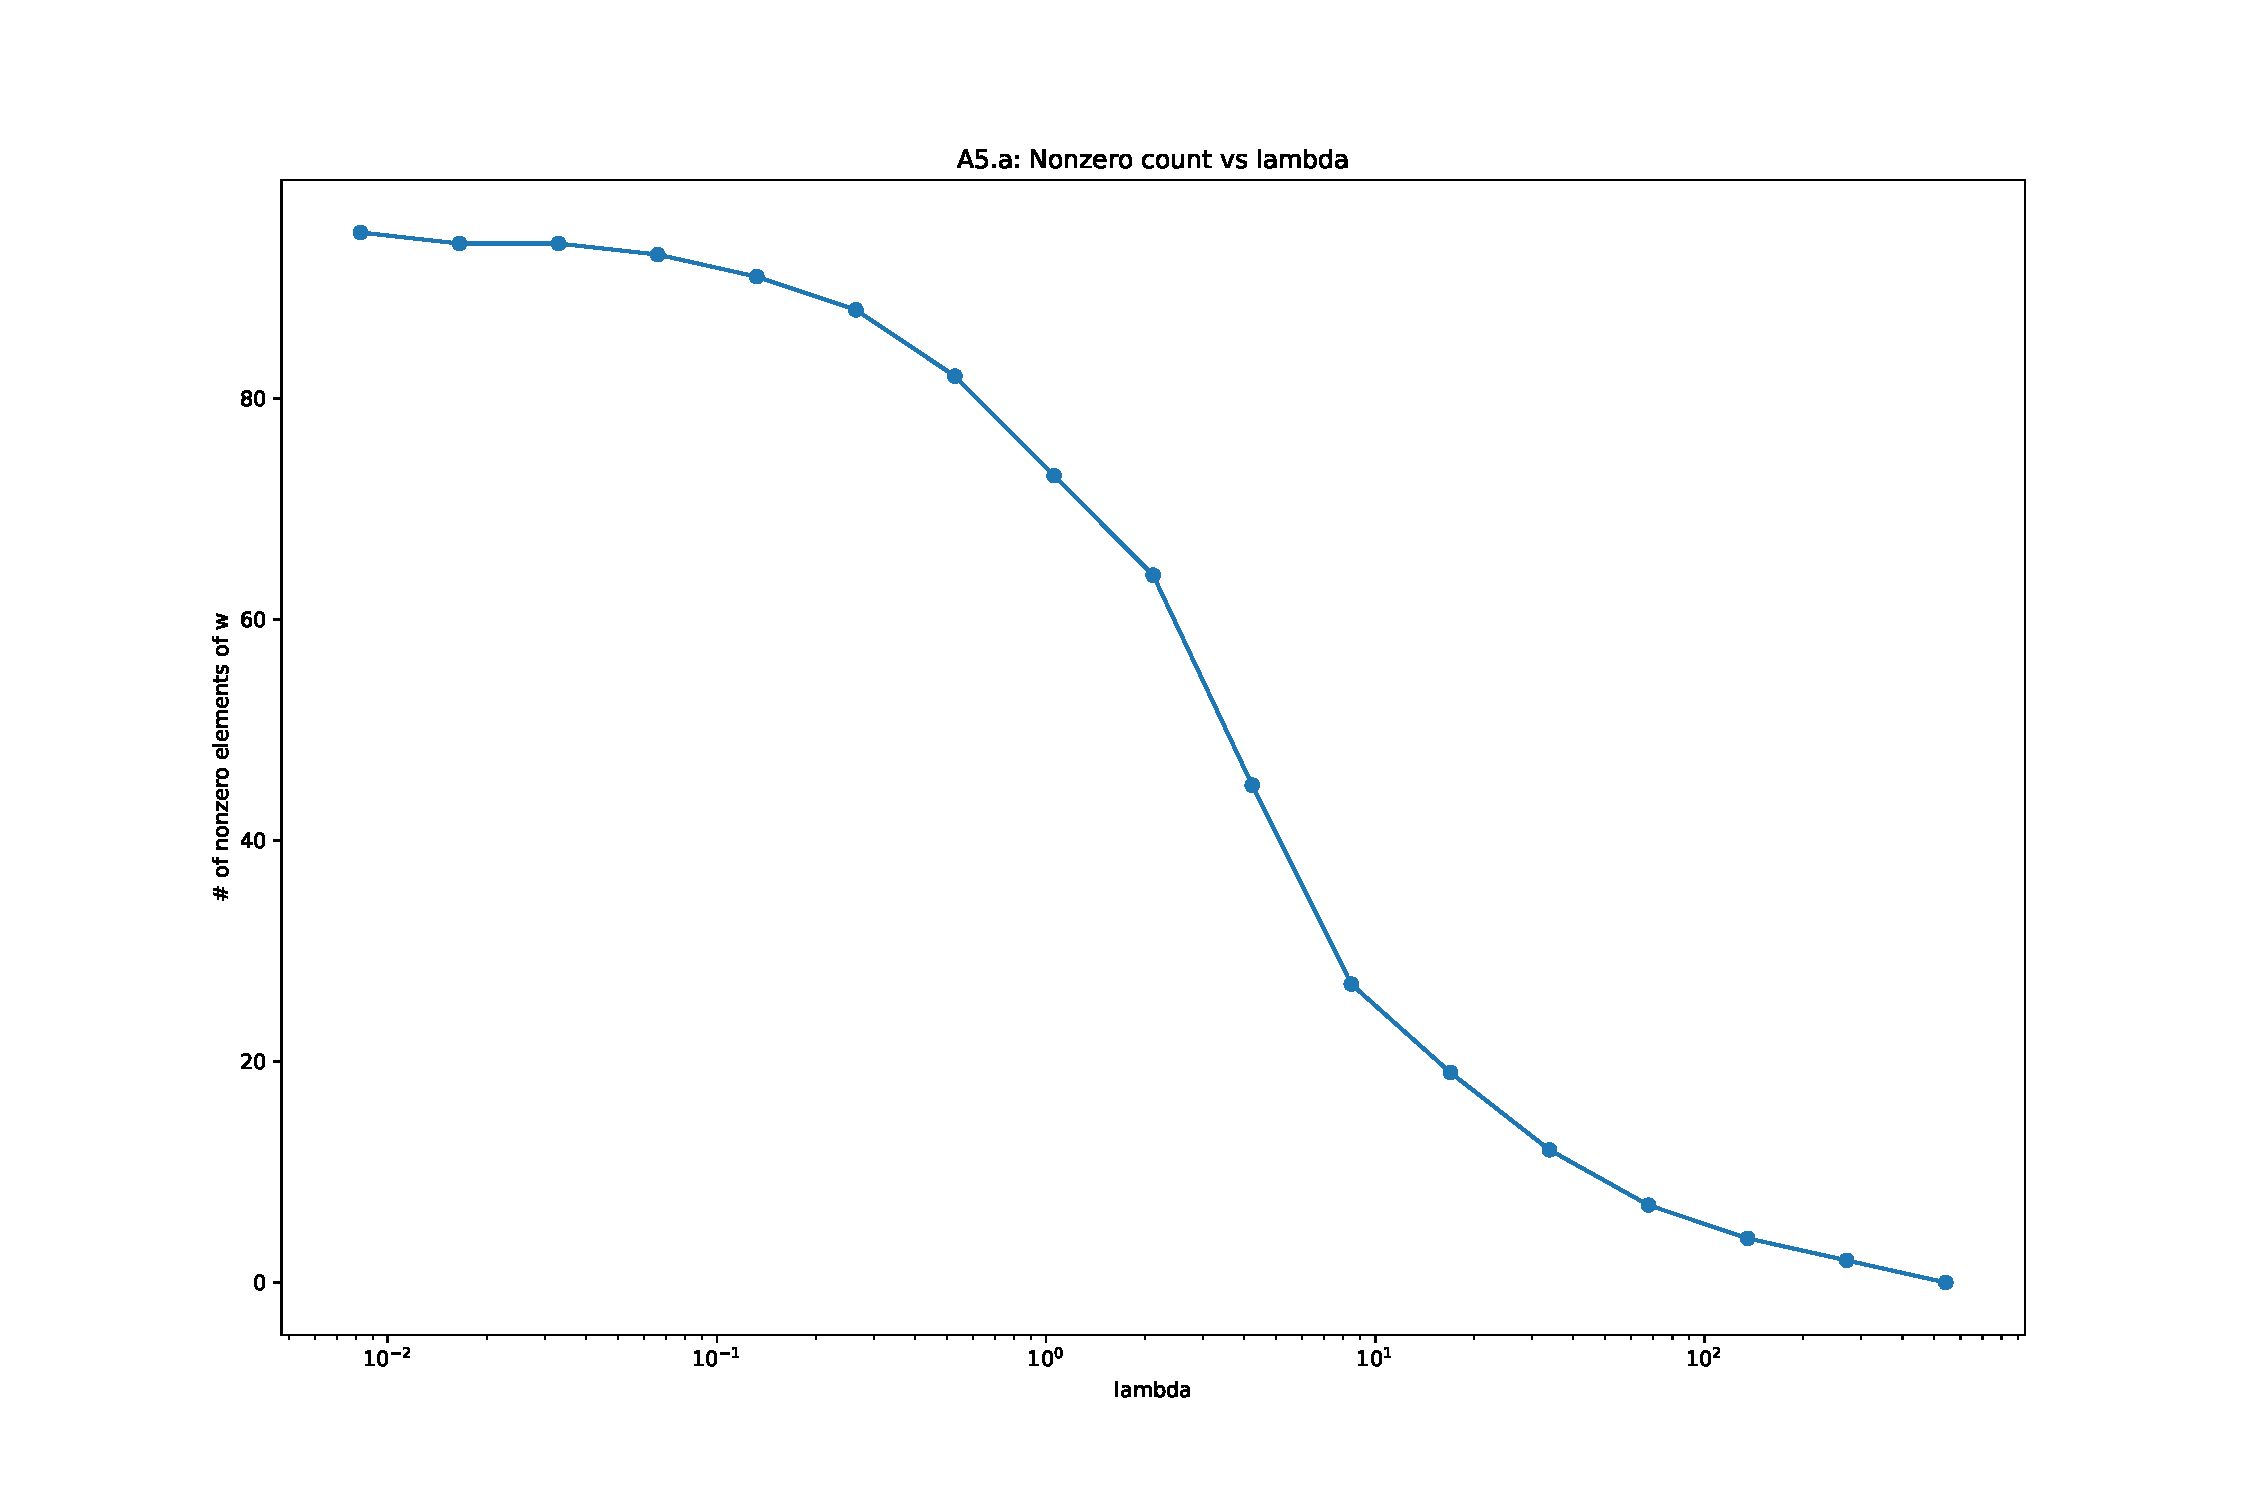
\includegraphics[width=0.49\textwidth]{hw2/code/figures/A5a.pdf}
            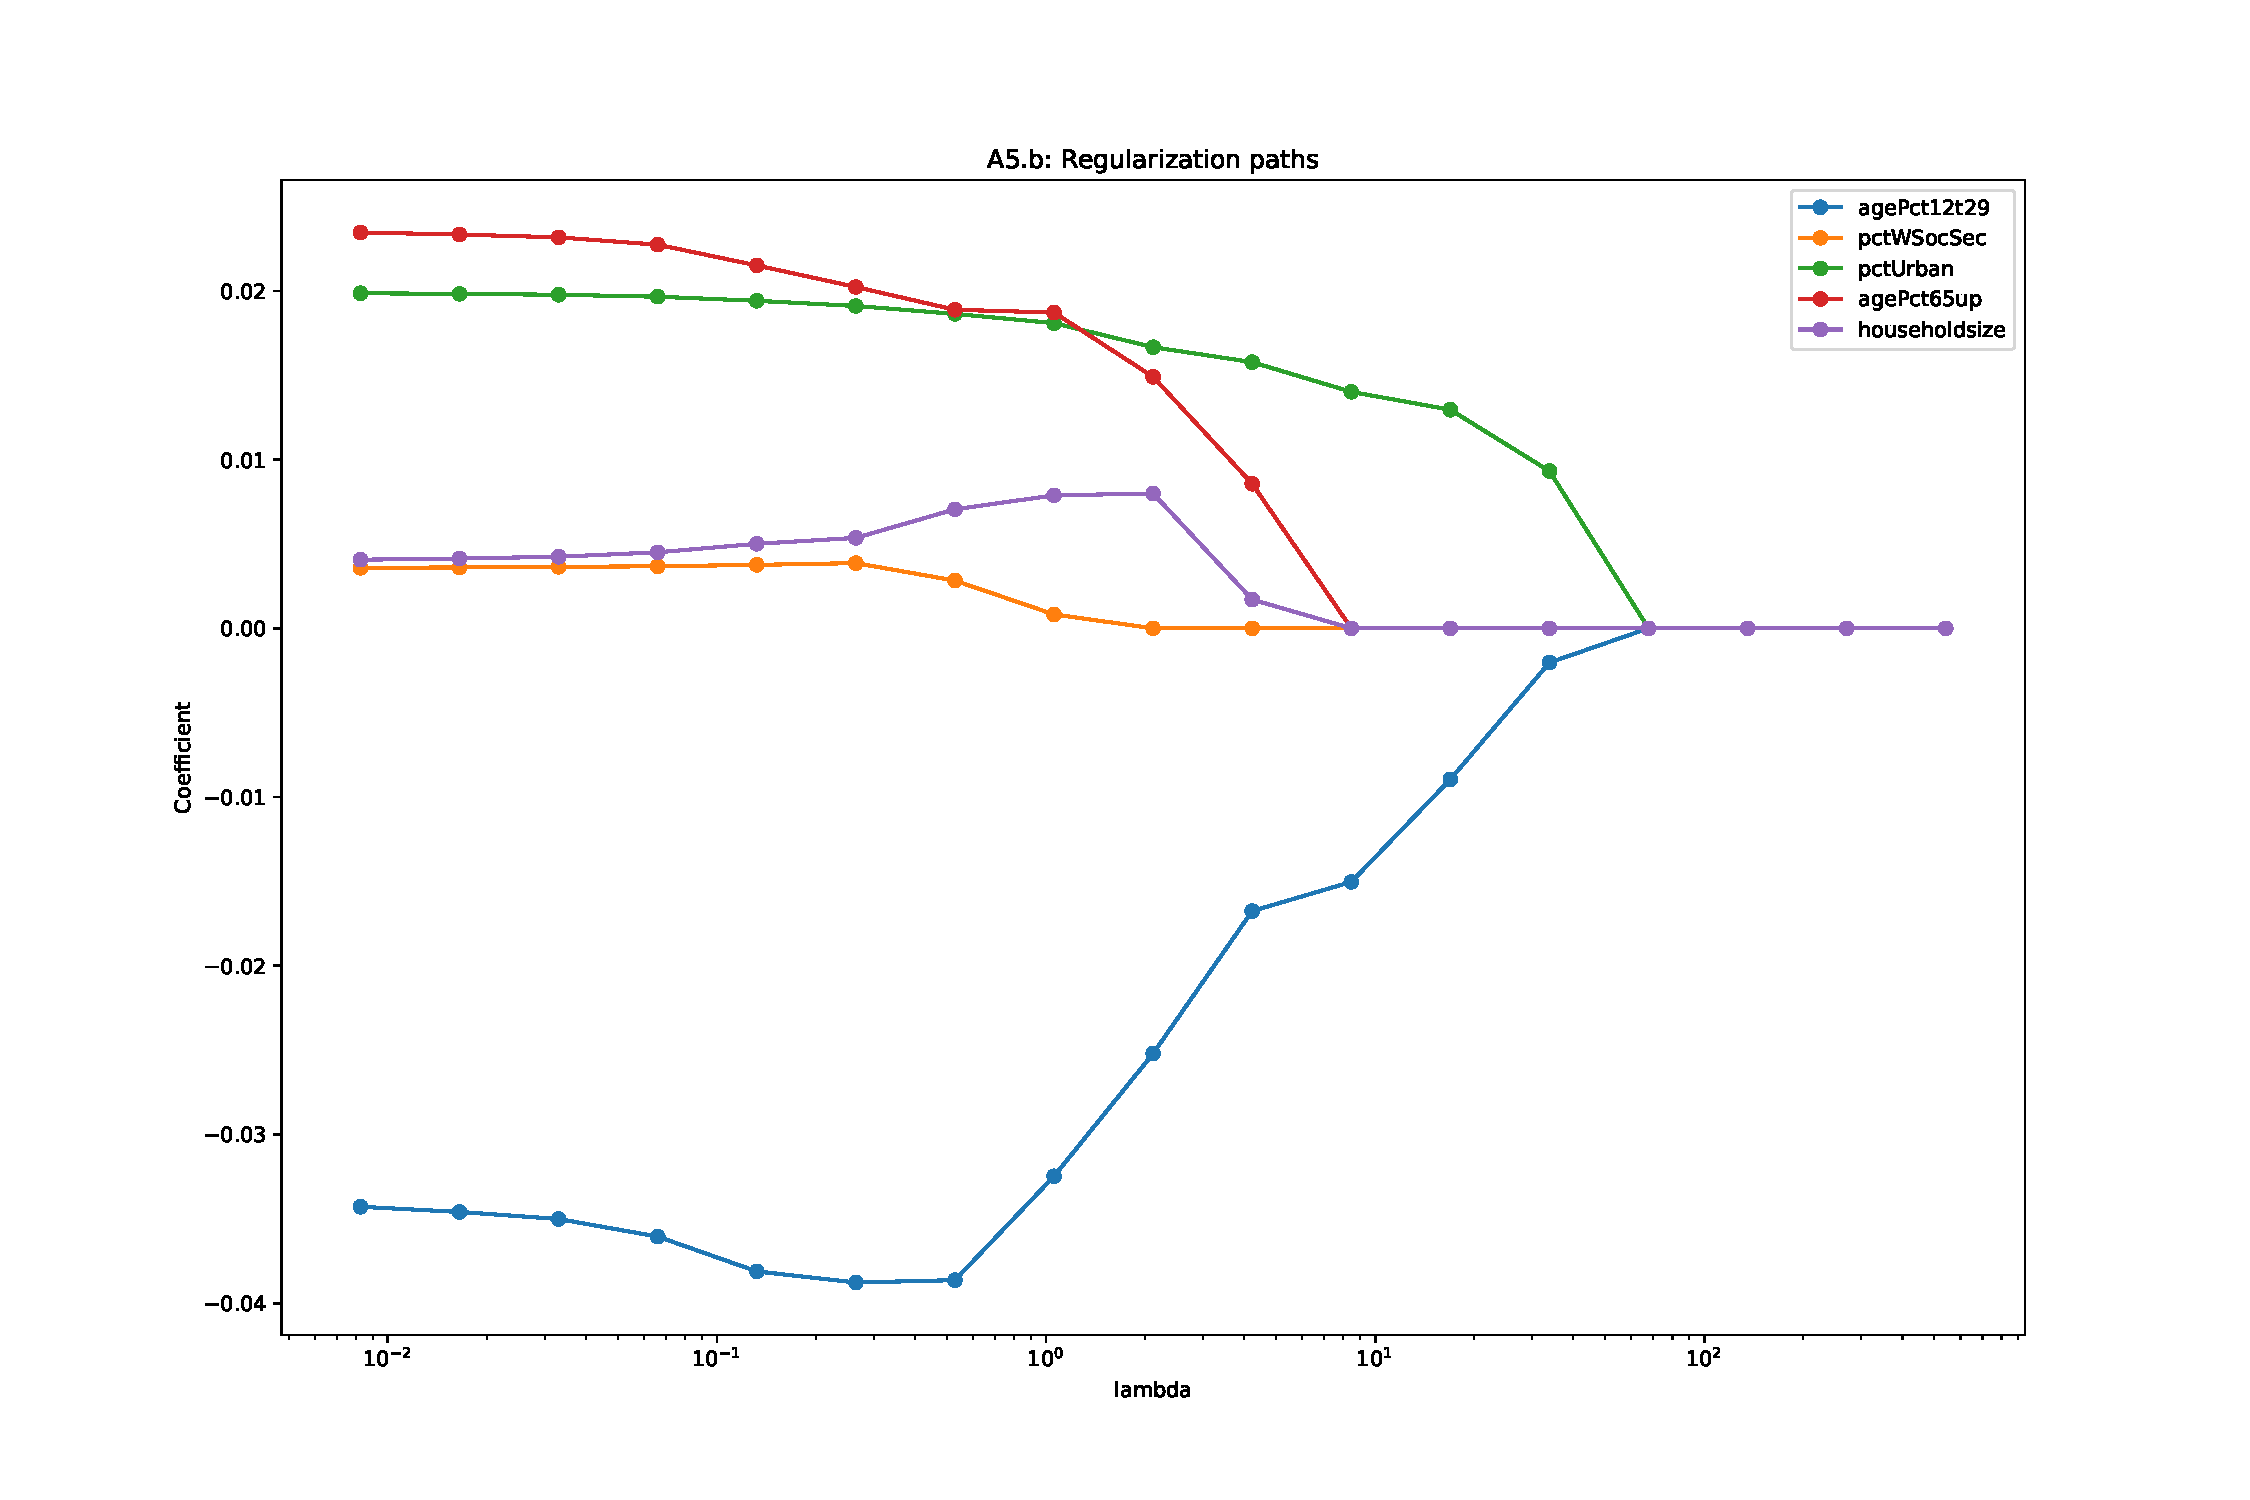
\includegraphics[width=0.49\textwidth]{hw2/code/figures/A5b.pdf}
            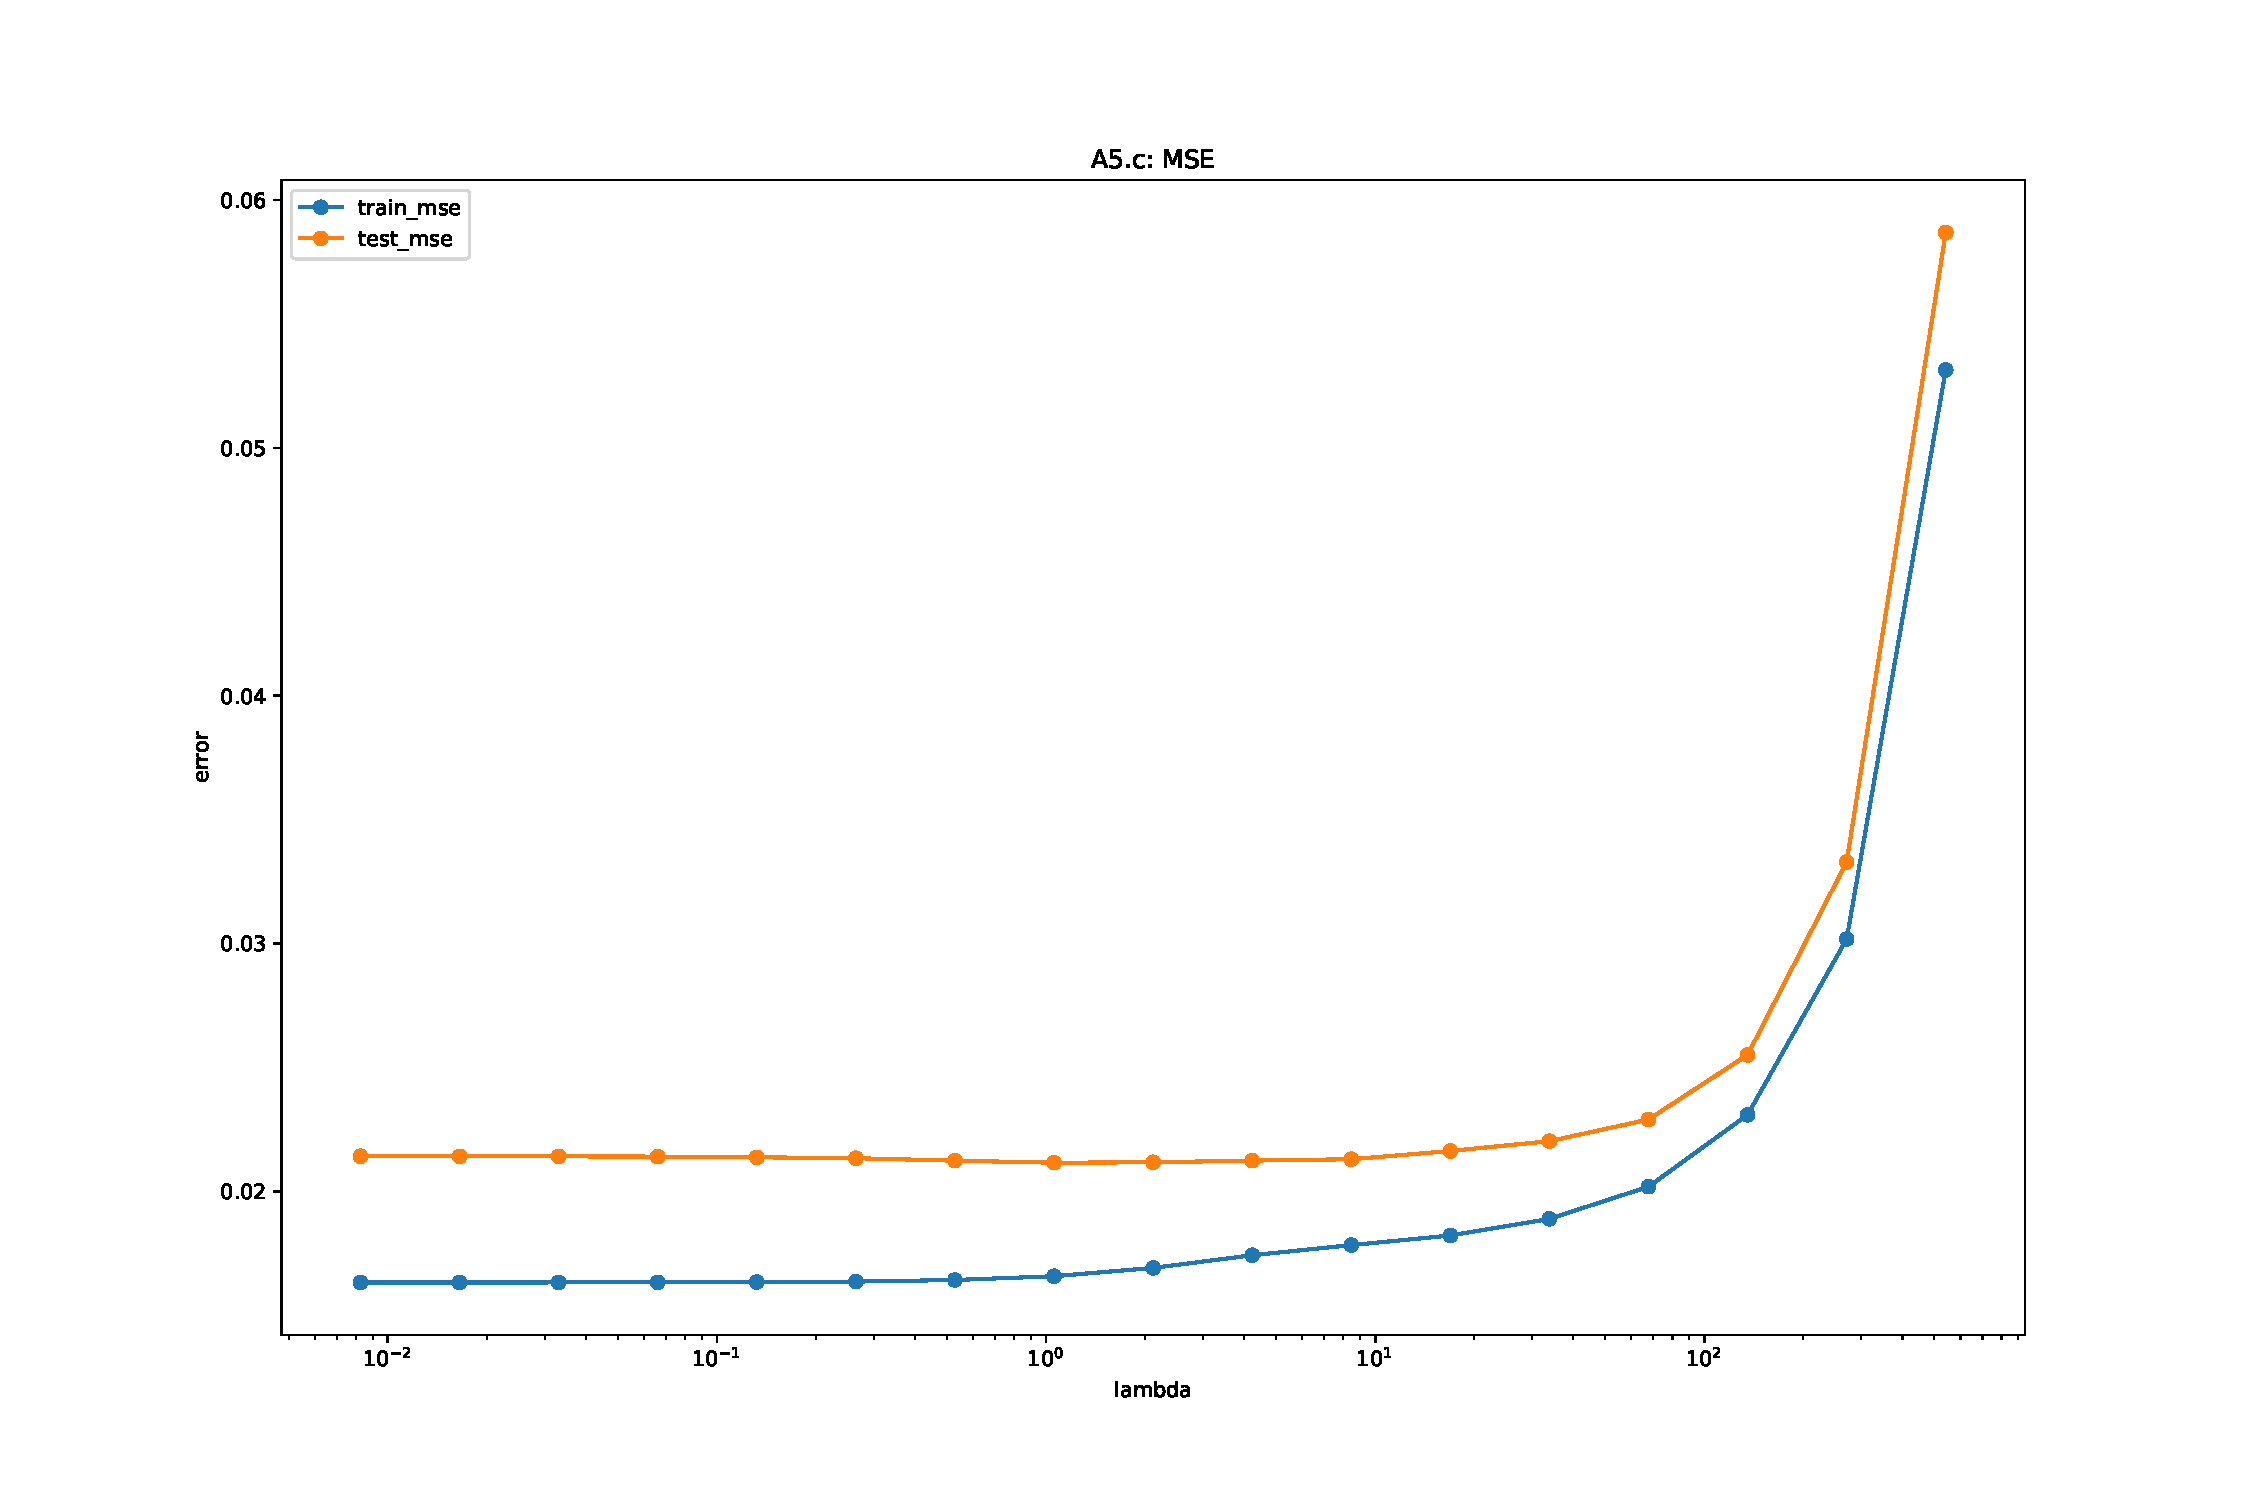
\includegraphics[width=0.5\textwidth]{hw2/code/figures/A5c.pdf}
            \caption{Problem A5. Top Left: A5.a, Top Right: A5.b, Bottom: A5.c}
            \label{figure:a4}
        \end{figure}
    \item The most positive weight: {\bf PctIlleg}\\
          The most negative weight: {\bf PctKids2Par}\\
          That is, the crime rate has the most positive correlation with PctIlleg (percentage of kids born to never married). On the other hand side, the crime rate has the most negative correlation with PctKids2Par (percentage of kids in family housing with two parents).
    \item Correlation is not the same with causality. Just because there are fewer people over 65 in the high crime areas, does not mean that the number of people over 65 decreases the crime rate. It could also mean that people over 65 tend to move out from high crime areas. Just like firetrucks don't cause fires. Seeing a fire truck is only correlated with seeing a burning building and it is the fire which causes the presence of a firetruck.

\end{enumerate}

\inputminted{python}{code/A5.py}
\caption{Code for A5}

\noindent\rule{\textwidth}{1pt}

\noindent\rule{\textwidth}{1pt}
A.6 {\bf Solution:}\\
\begin{enumerate}
    \item Note that $\exp(-y_i(b+x_i^Tw)) = \frac{1}{\mu_i(w,b)} -1$. Then, $\nabla_w J(w,b) = \frac{1}{n}\sum_i \nabla_w \log(1+\exp(-y_i(b+x_i^Tw))) + \nabla_w \lambda \|w\|^2 = \frac{1}{n}\sum_i \mu_i(w, b)(\frac{1}{\mu_i(w,b)} -1)(-y_i)x_i + 2\lambda w$. So
    $$
    \boxed{\nabla_w J(w,b) = \frac{1}{n}\sum_i (\mu_i(w, b) - 1)(y_i)x_i + 2\lambda w}
    $$
    Now, $\nabla_b J(w,b) = \frac{1}{n}\sum_i \nabla_b \log(1+\exp(-y_i(b+x_i^Tw))) + \nabla_b \lambda \|w\|^2 = \frac{1}{n}\sum_i \mu_i(w, b)(\frac{1}{\mu_i(w,b)} -1)(-y_i)$. So
    $$
    \boxed{\nabla_b J(w,b) = \frac{1}{n}\sum_i (\mu_i(w, b) - 1)y_i}
    $$
    \item See Figure 4. 
        \begin{figure}[h!]
            \centering
            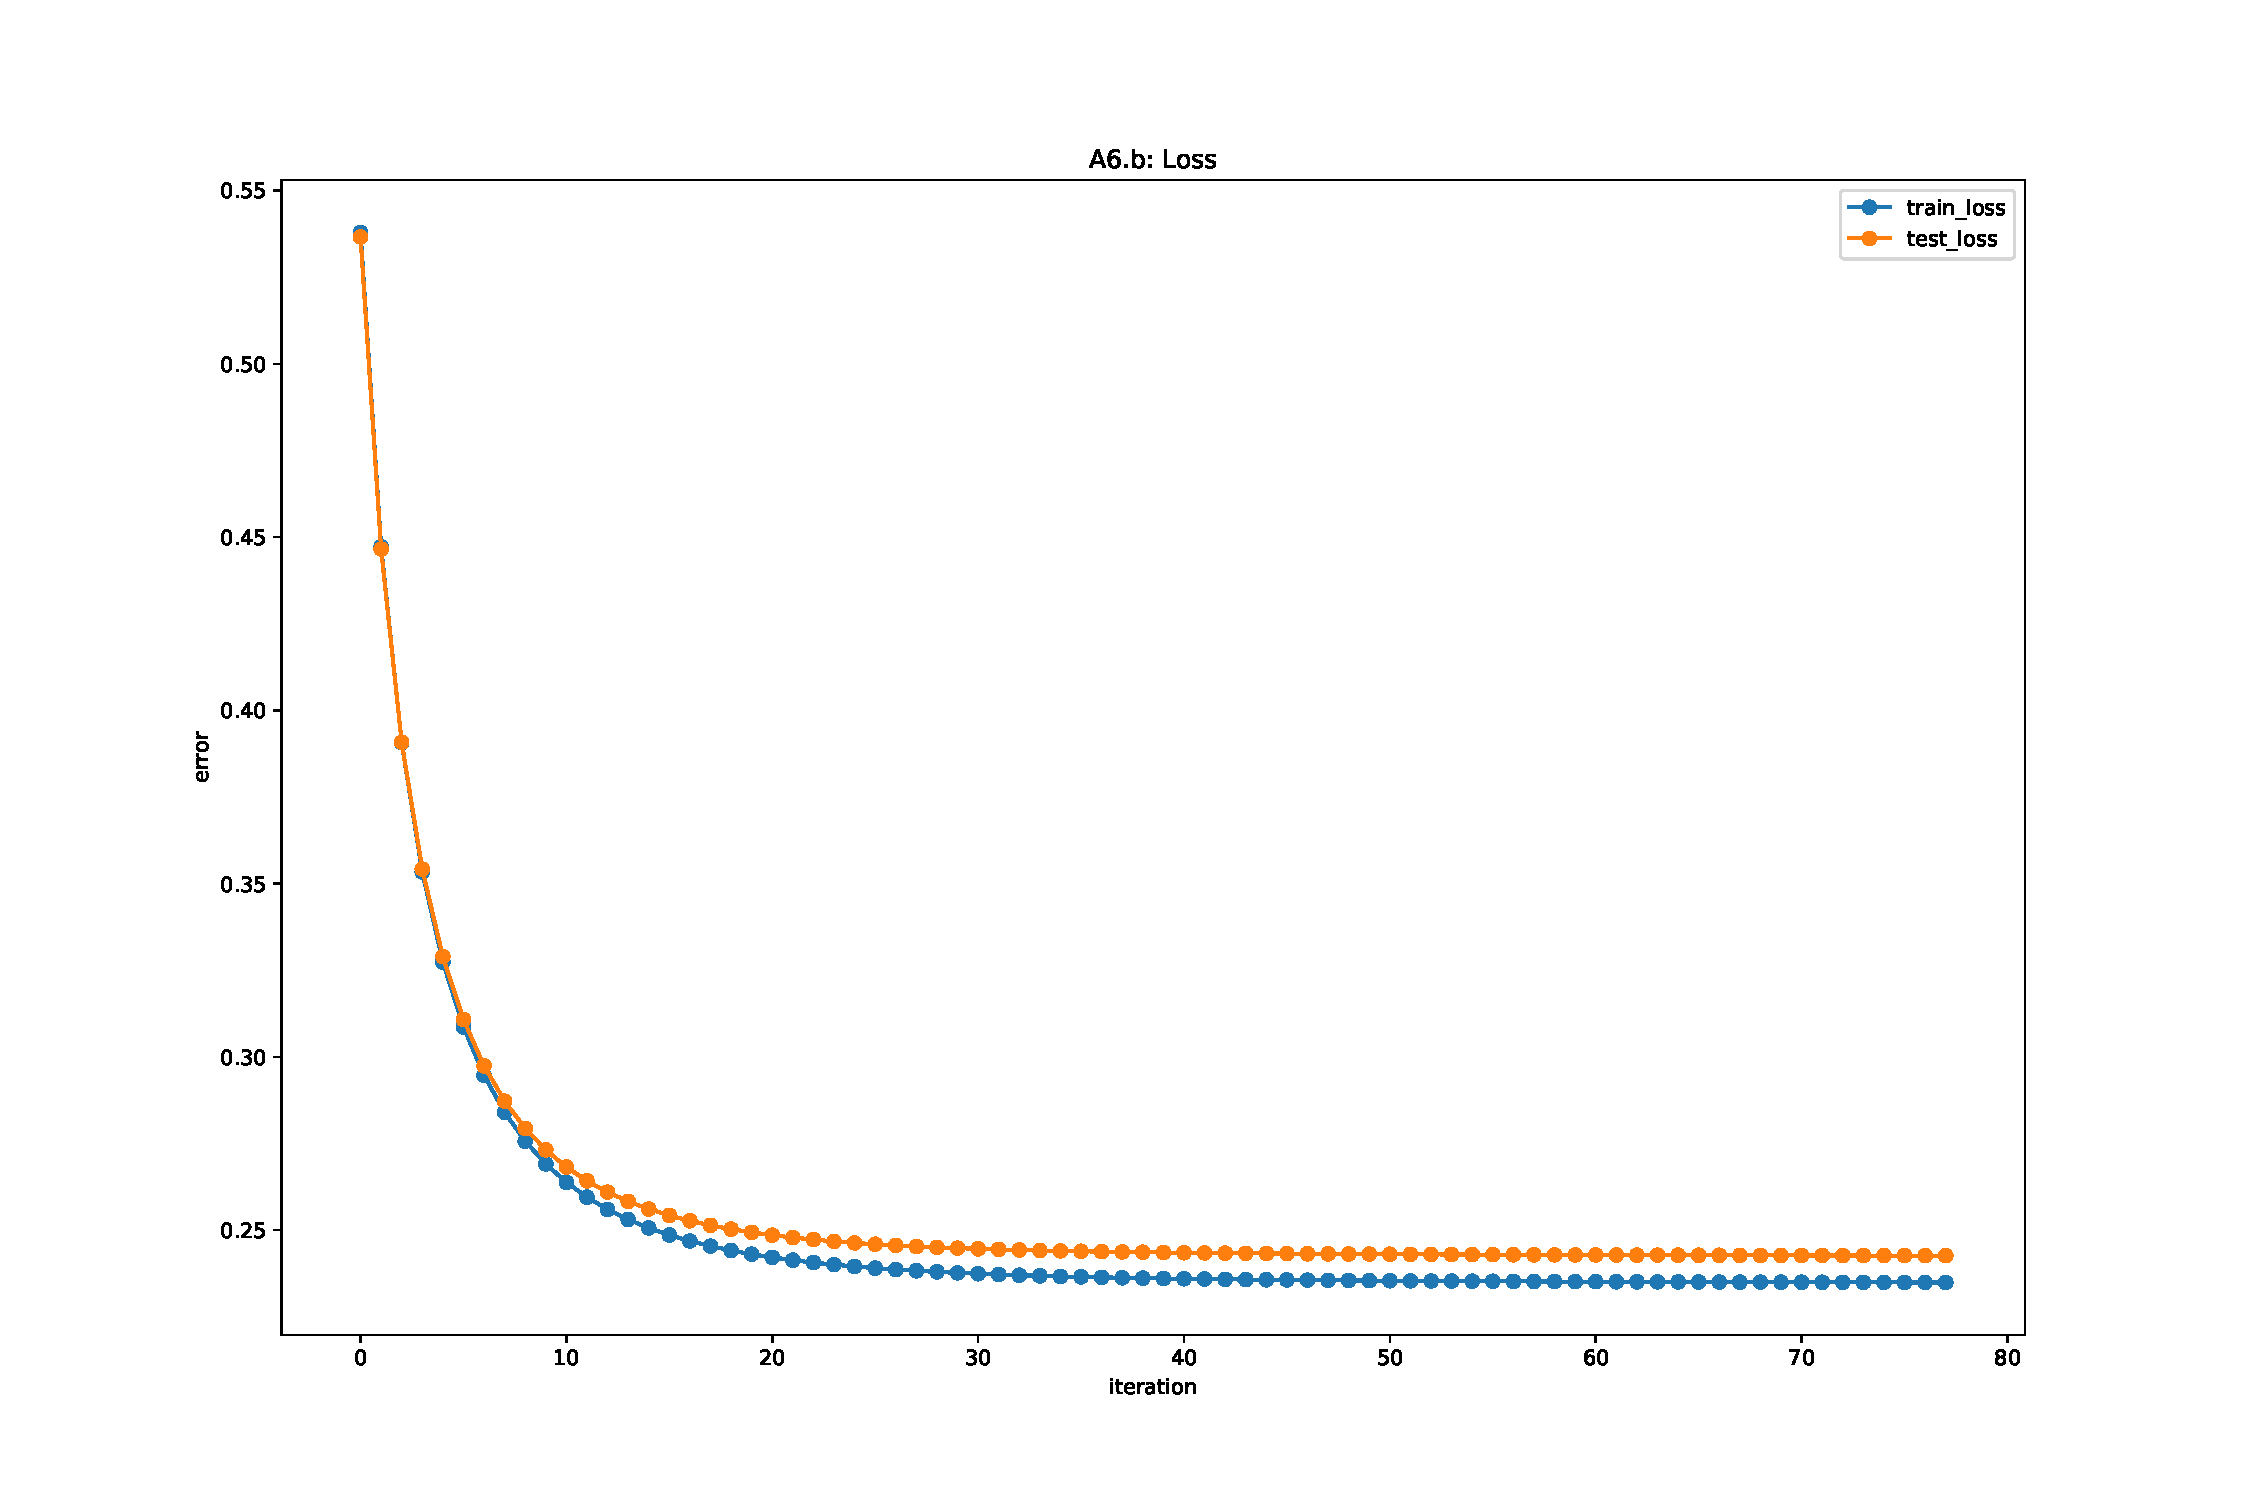
\includegraphics[width=0.49\textwidth]{hw2/code/figures/A6b1.pdf}
            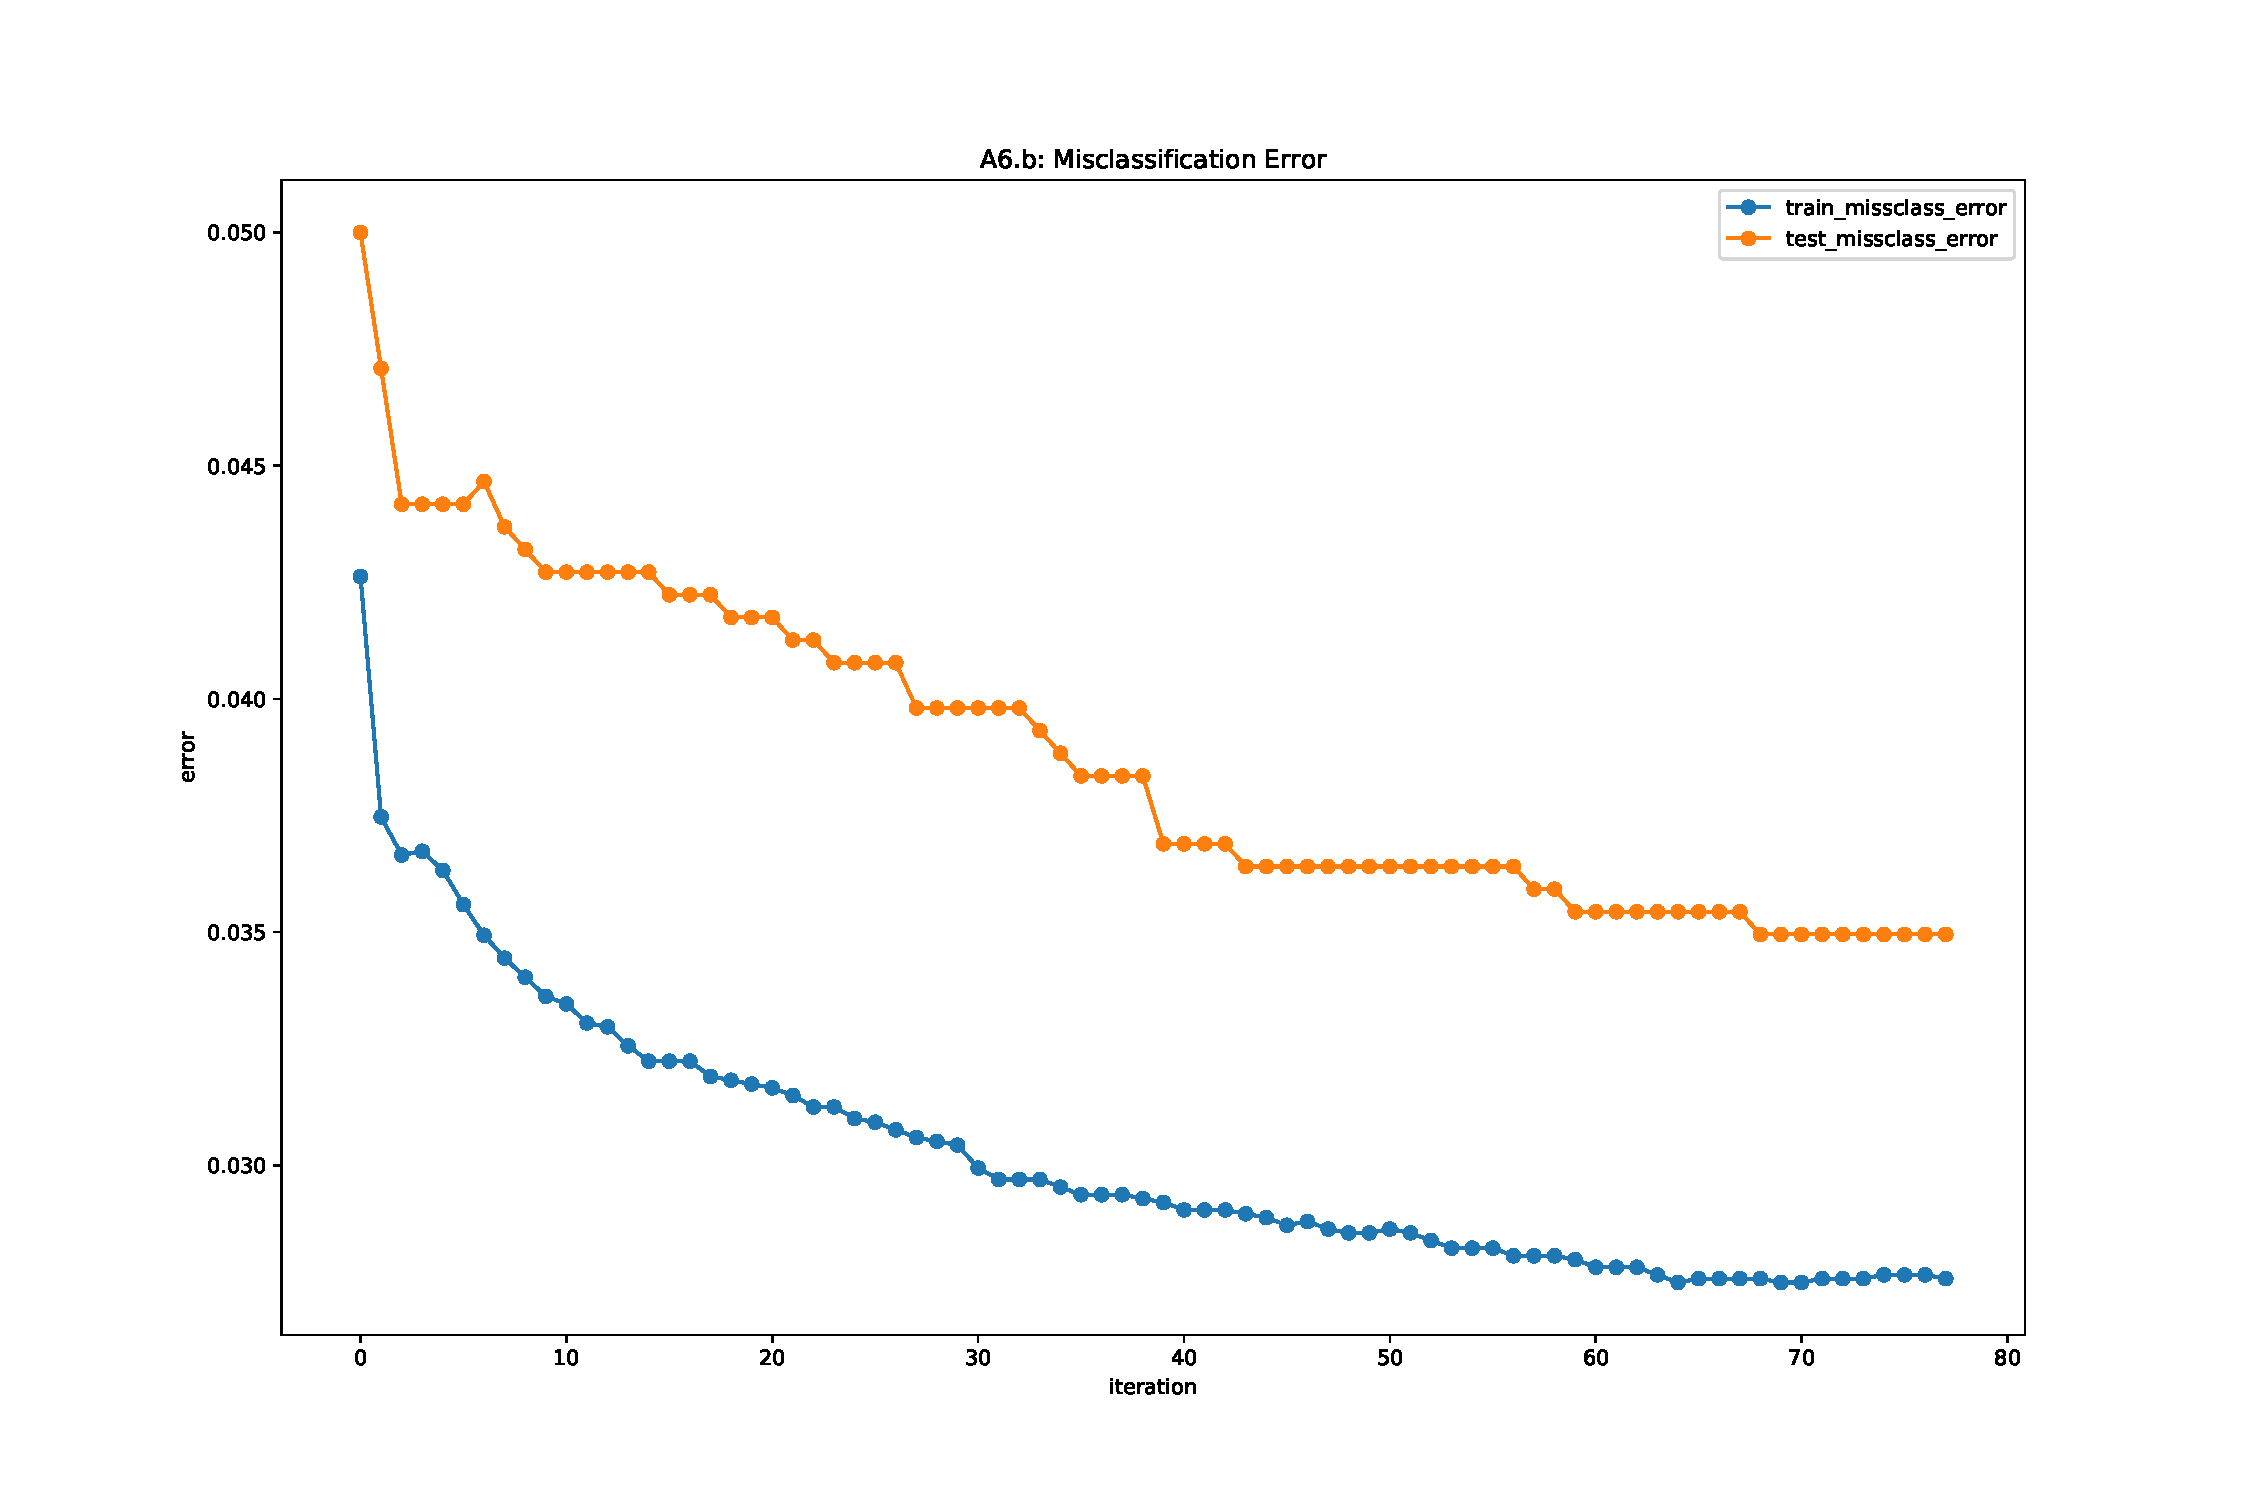
\includegraphics[width=0.49\textwidth]{hw2/code/figures/A6b2.pdf}
            \caption{Problem A6.b Left: A6.bi, Right: A6.bii (Plots for Gradient Descent)}
        \end{figure}
    \item See Figure 5. 
        \begin{figure}[h!]
            \centering
            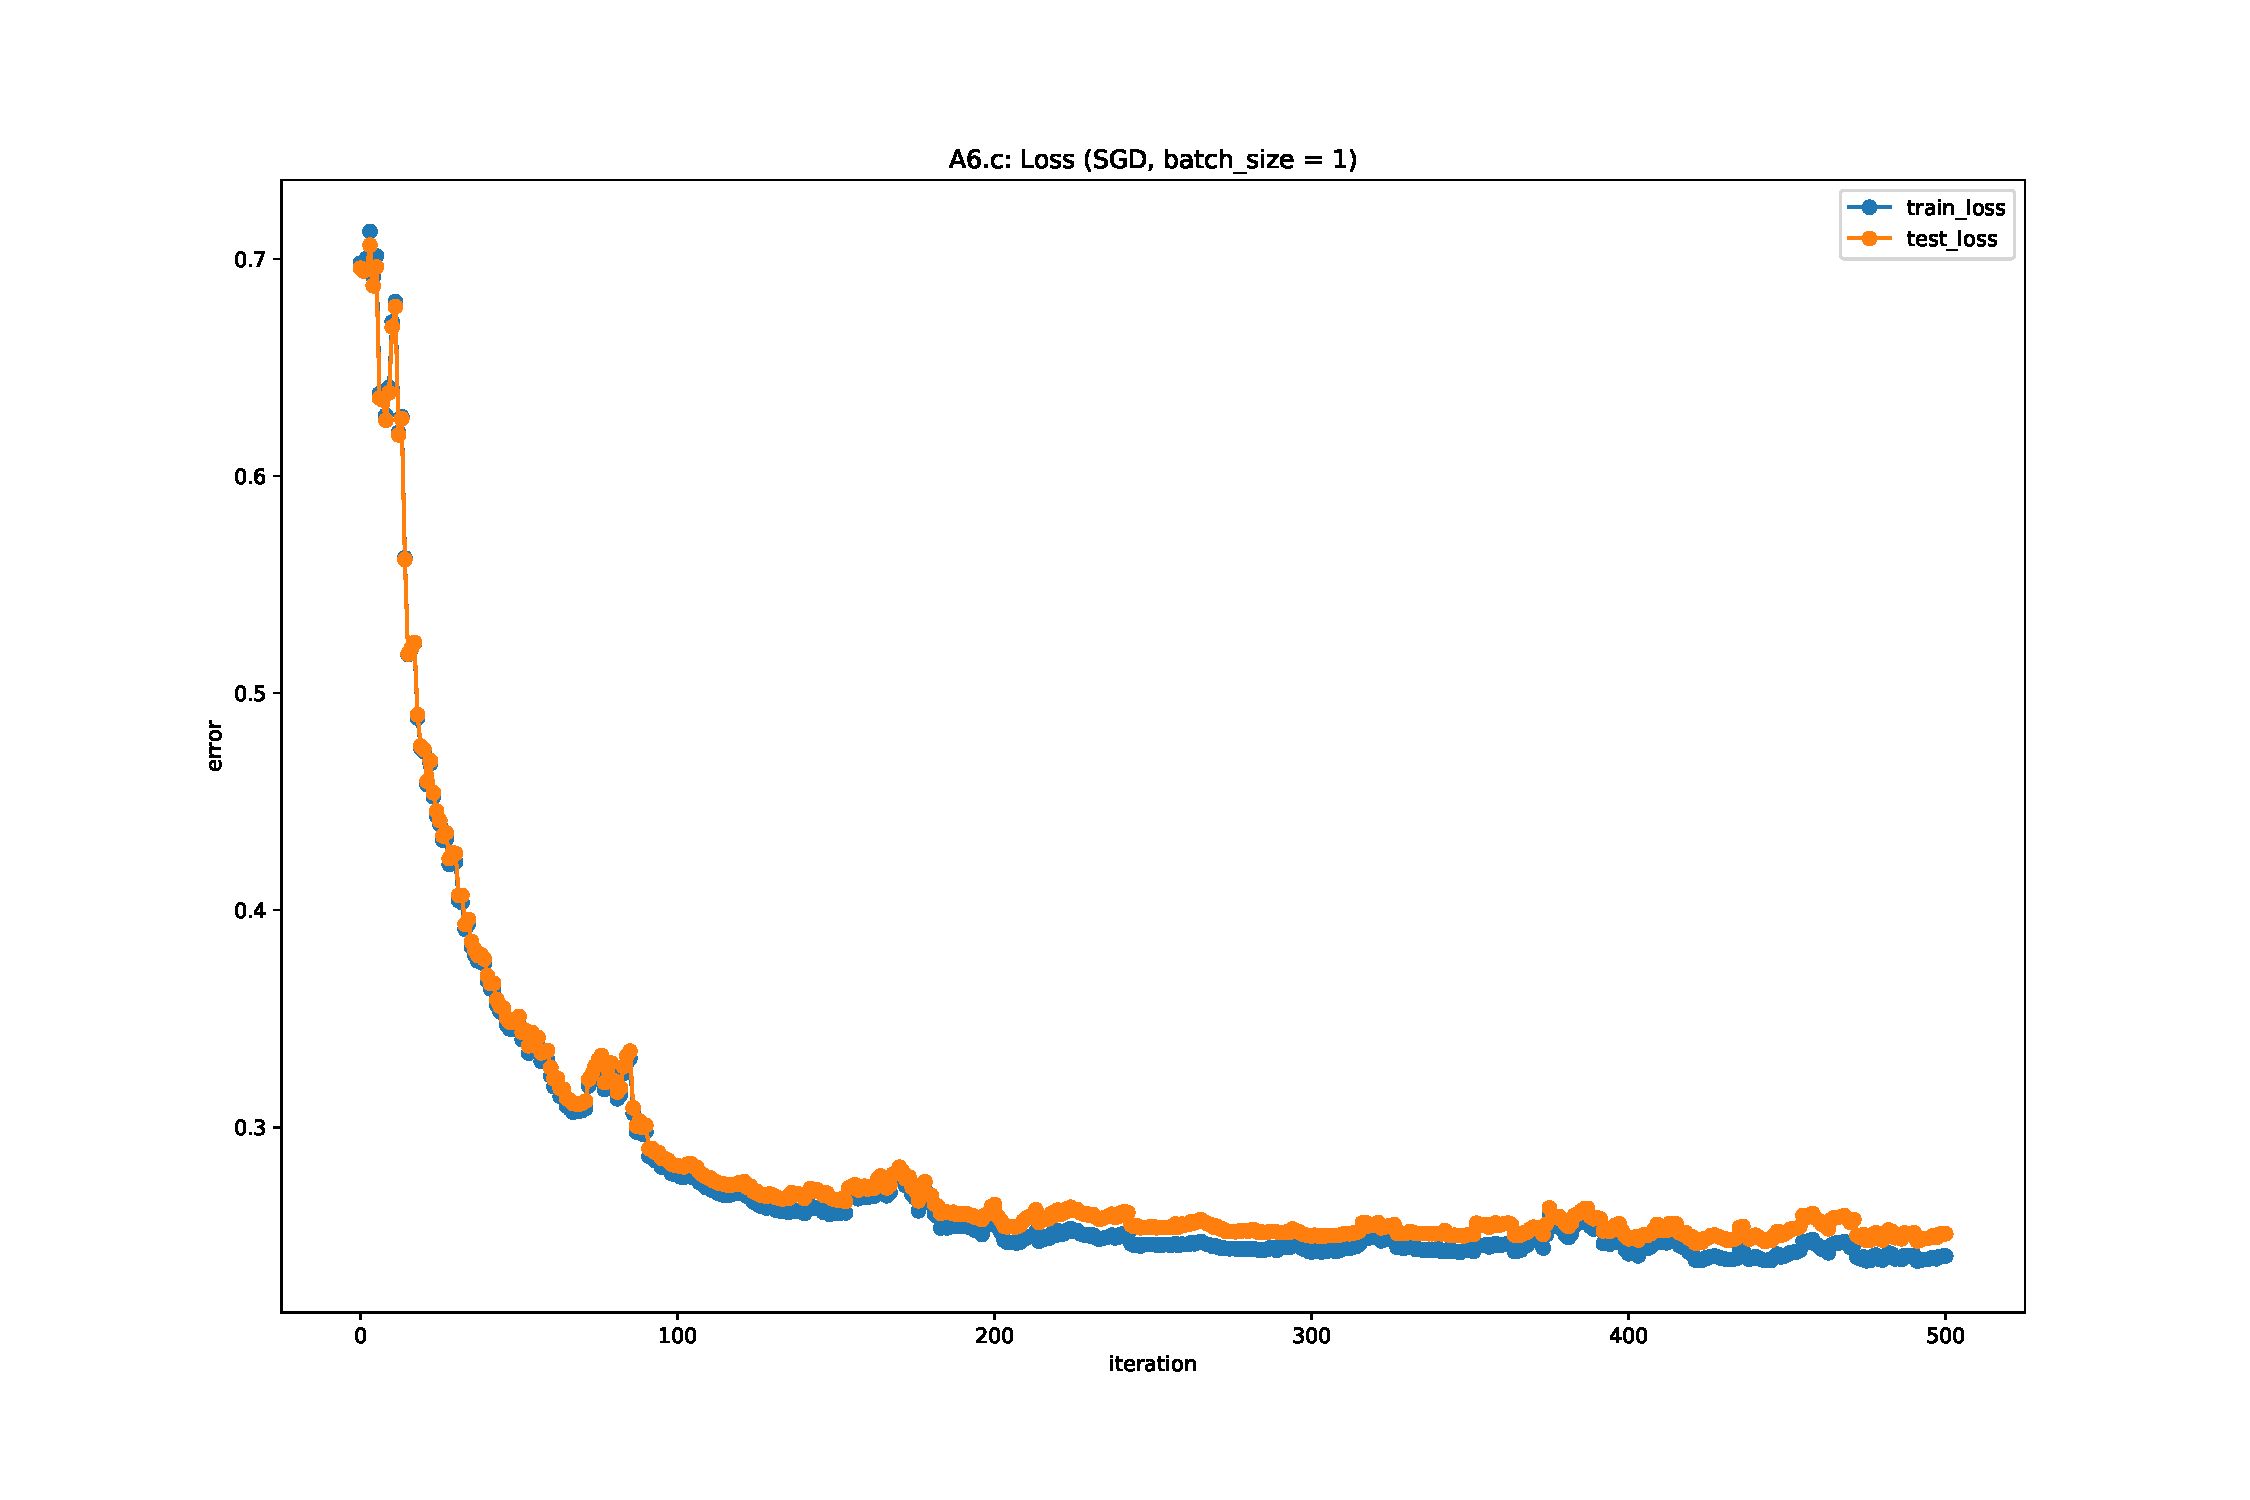
\includegraphics[width=0.49\textwidth]{hw2/code/figures/A6c1.pdf}
            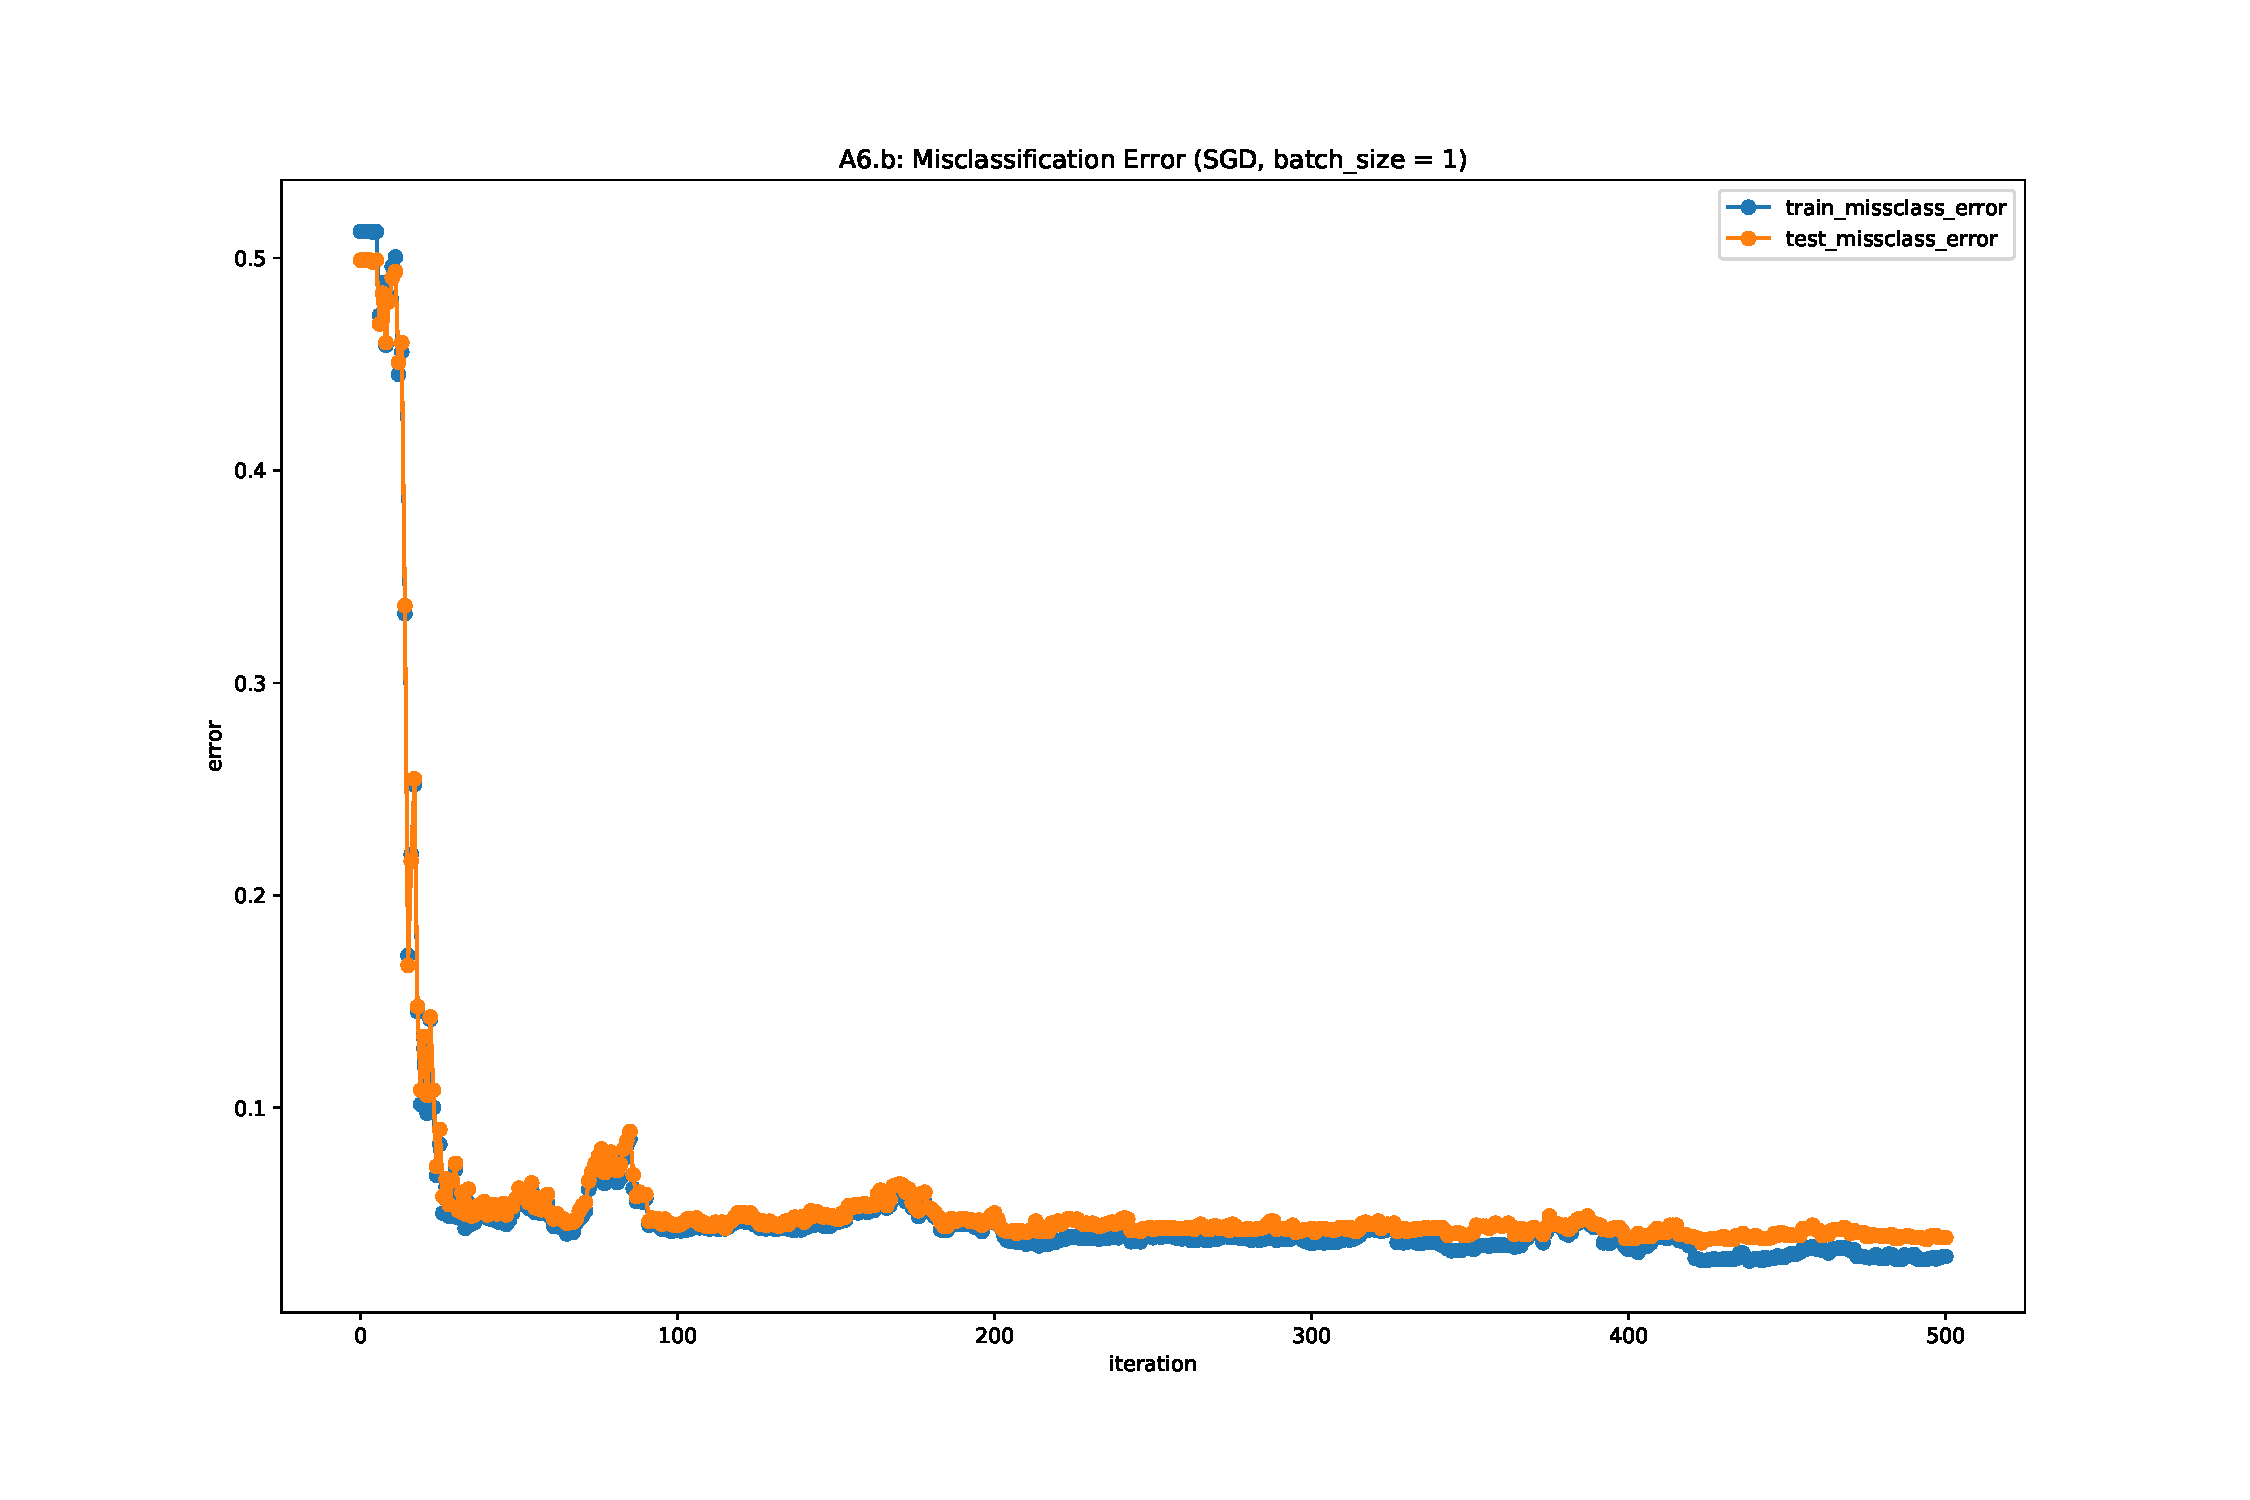
\includegraphics[width=0.49\textwidth]{hw2/code/figures/A6c2.pdf}
            \caption{Problem A6.c Left: A6.ci, Right: A6.cii (Plots for Stochastic Gradient Descent with batch 1.)}
        \end{figure}
        
    \item See Figure 6.
        \begin{figure}[h!]
            \centering
            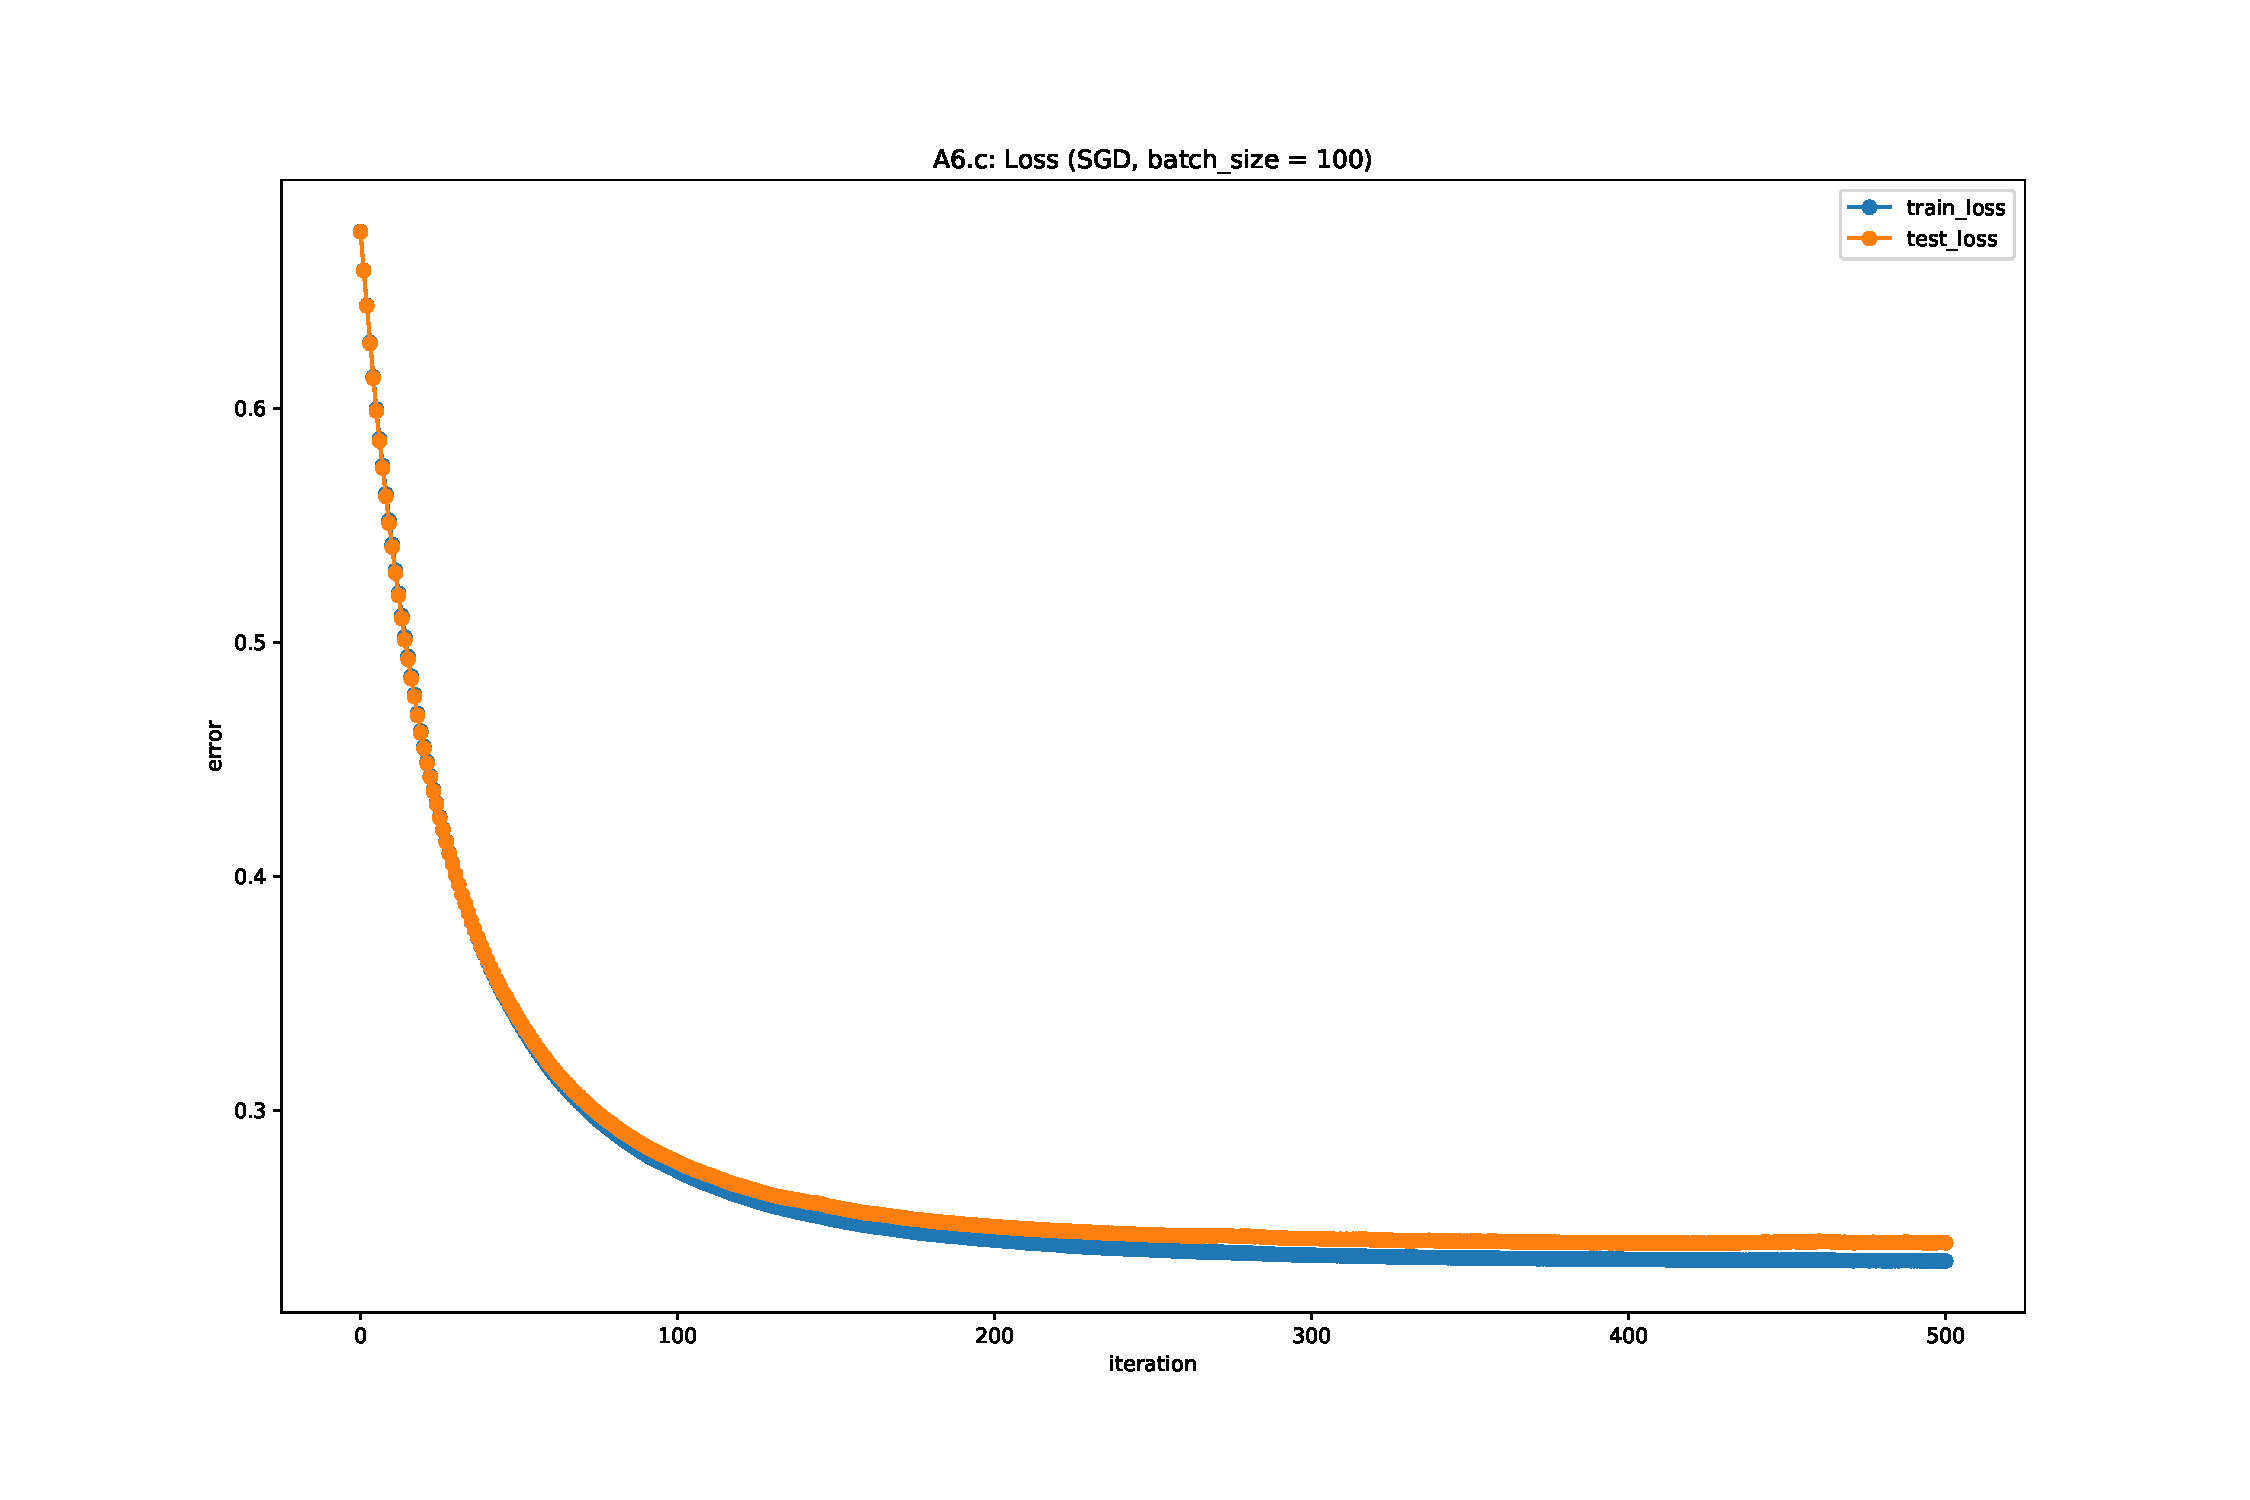
\includegraphics[width=0.49\textwidth]{hw2/code/figures/A6d1.pdf}
            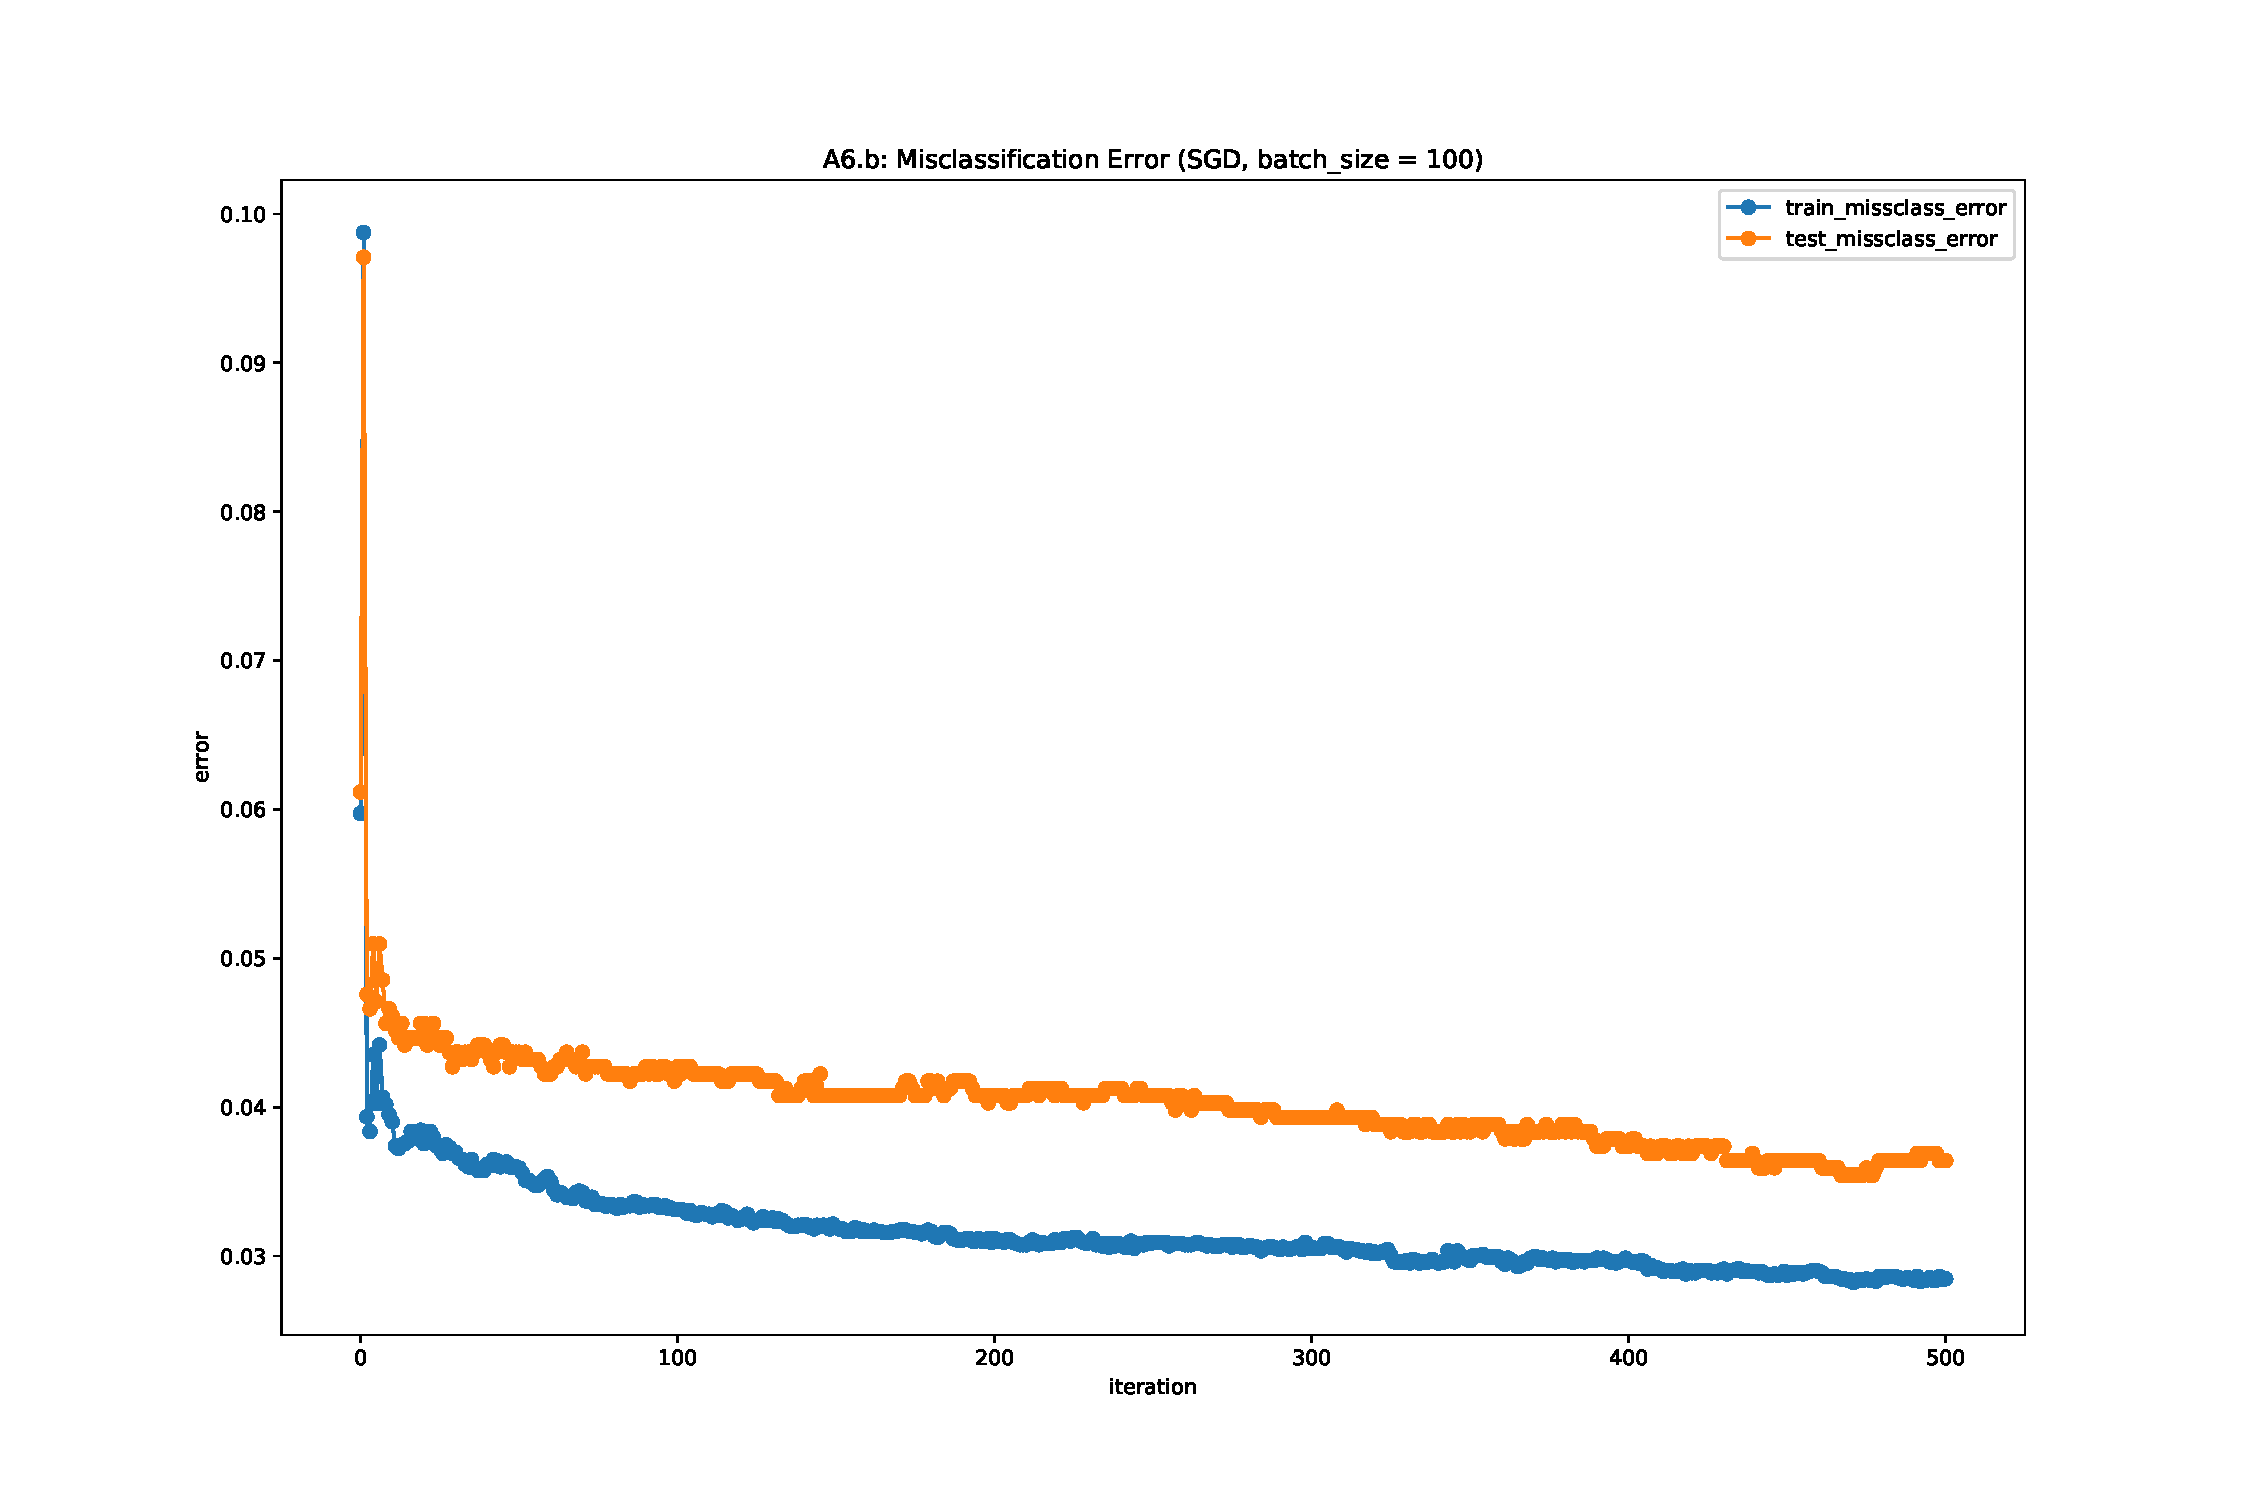
\includegraphics[width=0.49\textwidth]{hw2/code/figures/A6d2.pdf}
            \caption{Problem A6.d Left: A6.di, Right: A6.dii (Plots for Stochastic Gradient Descent with batch 100.)}
        \end{figure}

\end{enumerate}

\inputminted{python}{code/A6.py}
\caption{Code for A6}

\noindent\rule{\textwidth}{1pt}






\noindent\rule{\textwidth}{1pt}
B.4 {\bf Solution:}\\
\begin{enumerate}
    \item No time to explain!:)
    
    
    \item No time to explain!:)
    
    
    \item For Multinomial Logistic Regression trained with L(W) the train accuracy is 0.9127 and test accuracy is 0.9158. For J(W) these values are 0.8490 and 0.8537 respectively. Both models were trained for 50 epochs with learning rate $l = 0.01$. 
\end{enumerate}




\inputminted{python}{code/B4.py}
\caption{Code for B4}

\noindent\rule{\textwidth}{1pt}









\end{document}
